\documentclass[11pt,a4paper,dvipsnames,twosided]{article}
\usepackage[deliverable]{IOHKCoverPage}

% data for Deliverable header -- added by KH from an EU H2020 project template
\DeliverableNumber{SL-D5}
\DeliverableTitle{A Formal Specification of the Cardano Ledger}{Formal Cardano Ledger Spec.}
\DeliverableResponsible{Formal Methods Team}
\EditorName{Jared Corduan, \IOHK}
\Authors{Jared Corduan \quad \texttt{<jared.corduan@iohk.io>}
   \\[1em]
   Polina Vinogradova \quad \texttt{<polina.vinogradova@iohk.io>}
   \\[1em]
   Matthias G\"udemann \quad \texttt{<matthias.gudemann@iohk.io>}
}
\DueDate{15$^{\textrm{th}}$ October 2019}
\SubmissionDate{8th October 2019}{2019/10/08}
\LeaderName{Philipp Kant, \IOHK}
\InstitutionAddress{\IOHK}
\Version{1.0}
\Project{Shelley Ledger}
\DisseminationPU

\usepackage[margin=2.5cm]{geometry}
\usepackage{lscape}
\usepackage{iohk}
\usepackage{microtype}
\usepackage{mathpazo} % nice fonts
\usepackage{amsmath}
\usepackage{amssymb}
\usepackage{amsthm}
\usepackage{latexsym}
\usepackage{mathtools}
\usepackage{stmaryrd}
\usepackage{extarrows}
\usepackage{slashed}
\usepackage[unicode=true,pdftex,pdfa,colorlinks=true]{hyperref}
\usepackage{xcolor}
\usepackage[capitalise,noabbrev,nameinlink]{cleveref}
\usepackage{float}
\floatstyle{boxed}
\restylefloat{figure}
\usepackage{tikz}
\usepackage{booktabs}
\usepackage{enumerate}
\usepackage{listings}
%%
%% Package `semantic` can be used for writing inference rules.
%%
\usepackage{semantic}
%% Setup for the semantic package
\setpremisesspace{20pt}

\usepackage{tocloft}
\addtolength{\cftsubsecnumwidth}{5pt}

%%
%% Types
%%
\newcommand{\Nothing}{\ensuremath{\Diamond}}
\newcommand{\N}{\ensuremath{\mathbb{N}}}
\newcommand{\Bool}{\type{Bool}}
\newcommand{\Npos}{\ensuremath{\mathbb{N}^{>0}}}
\newcommand{\Z}{\ensuremath{\mathbb{Z}}}
\newcommand{\Q}{\ensuremath{\mathbb{Q}}}
\newcommand{\R}{\ensuremath{\mathbb{R}}}
\newcommand{\Rnn}{\ensuremath{\mathbb{R}^{\geq 0}}}
\newcommand{\Tx}{\type{Tx}}
\newcommand{\TxBody}{\type{TxBody}}
\newcommand{\TxWitness}{\type{TxWitness}}
\newcommand{\Ix}{\type{Ix}}
\newcommand{\TxId}{\type{TxId}}
\newcommand{\Addr}{\type{Addr}}
\newcommand{\UTxO}{\type{UTxO}}
\newcommand{\Wdrl}{\type{Wdrl}}
\newcommand{\Coin}{\type{Coin}}
\newcommand{\PParams}{\type{PParams}}
\newcommand{\PParamsUpdate}{\type{PParamsUpdate}}
\newcommand{\ProposedPPUpdates}{\type{ProposedPPUpdates}}
\newcommand{\Slot}{\type{Slot}}
\newcommand{\StabilityWindow}{\ensuremath{\mathsf{StabilityWindow}}}
\newcommand{\RandomnessStabilisationWindow}{\ensuremath{\mathsf{RandomnessStabilisationWindow}}}
\newcommand{\SlotsPerEpoch}{\mathsf{SlotsPerEpoch}}
\newcommand{\SlotsPerKESPeriod}{\mathsf{SlotsPerKESPeriod}}
\newcommand{\MaxMajorPV}{\mathsf{MaxMajorPV}}
\newcommand{\ActiveSlotCoeff}{\mathsf{ActiveSlotCoeff}}
\newcommand{\Network}{\mathsf{Network}}
\newcommand{\NetworkId}{\mathsf{NetworkId}}
\newcommand{\BlockNo}{\type{BlockNo}}
\newcommand{\MaxKESEvo}{\ensuremath{\mathsf{MaxKESEvo}}}
\newcommand{\Quorum}{\ensuremath{\mathsf{Quorum}}}
\newcommand{\MaxLovelaceSupply}{\ensuremath{\mathsf{MaxLovelaceSupply}}}
\newcommand{\Duration}{\type{Duration}}
\newcommand{\StakePools}{\type{StakePools}}
\newcommand{\Seed}{\type{Seed}}
\newcommand{\seedOp}{\star}
\newcommand{\Ppm}{\type{Ppm}}
\newcommand{\ProtVer}{\ensuremath{\type{ProtVer}}}
\newcommand{\Metadatum}{\ensuremath{\type{Metadatum}}}
\newcommand{\Metadata}{\ensuremath{\type{Metadata}}}
\newcommand{\MetadataHash}{\ensuremath{\type{MetadataHash}}}
\newcommand{\Update}{\type{Update}}
\newcommand{\GenesisDelegation}{\type{GenesisDelegation}}
\newcommand{\FutGenesisDelegation}{\type{FutGenesisDelegation}}

\newcommand{\DCert}{\type{DCert}}
\newcommand{\DCertRegKey}{\type{DCert_{regkey}}}
\newcommand{\DCertDeRegKey}{\type{DCert_{deregkey}}}
\newcommand{\DCertDeleg}{\type{DCert_{delegate}}}
\newcommand{\DCertRegPool}{\type{DCert_{regpool}}}
\newcommand{\DCertRetirePool}{\type{DCert_{retirepool}}}
\newcommand{\DCertGen}{\type{DCert_{genesis}}}
\newcommand{\DCertMir}{\type{DCert_{mir}}}
\newcommand{\PoolParam}{\type{PoolParam}}
\newcommand{\PoolMD}{\type{PoolMD}}
\newcommand{\MIRPot}{\type{MIRPot}}
\newcommand{\InstantaneousRewards}{\type{InstantaneousRewards}}
\newcommand{\ReservesMIR}{\type{ReservesMIR}}
\newcommand{\TreasuryMIR}{\type{TreasuryMIR}}
\newcommand{\URL}{\type{Url}}
\newcommand{\UTxOState}{\ensuremath{\type{UTxOState}}}
\newcommand{\ledgerState}{\ensuremath{\type{ledgerState}}}

\newcommand{\AddrRWD}{\type{Addr_{rwd}}}
\newcommand{\AddrB}{\type{Addr_{base}}}
\newcommand{\AddrP}{\type{Addr_{ptr}}}
\newcommand{\AddrE}{\type{Addr_{enterprise}}}
\newcommand{\AddrBS}{\type{Addr_{bootstrap}}}
\newcommand{\Ptr}{\type{Ptr}}
\newcommand{\DState}{\type{DState}}
\newcommand{\DWEnv}{\type{DWEnv}}
\newcommand{\DPSEnv}{\type{DPSEnv}}
\newcommand{\DPEnv}{\type{DPEnv}}
\newcommand{\DEnv}{\type{DEnv}}
\newcommand{\PEnv}{\type{PEnv}}
\newcommand{\DPState}{\type{DPState}}
\newcommand{\PState}{\type{PState}}
\newcommand{\DCertBody}{\type{DCertBody}}
\newcommand{\TData}{\type{TData}}
\newcommand{\DPoolReap}{\ensuremath{\type{poolreap}}}
\newcommand{\UPIState}{\type{UPIState}}
\newcommand{\UpdatePayload}{\type{UpdatePayload}}

% multi-signature
\newcommand{\StakeCredential}{\type{Credential}_{stake}}

\newcommand{\txwitsVKey}[1]{\fun{txwitsVKey}~\var{#1}}
\newcommand{\txwitsScript}[1]{\fun{txwitsScript}~\var{#1}}

\newcommand{\AddrVKey}{\type{Addr^{vkey}}}
\newcommand{\AddrRWDVKey}{\type{Addr_{rwd}^{vkey}}}
\newcommand{\AddrRWDScr}{\type{Addr_{rwd}^{script}}}
\newcommand{\AddrVKeyB}{\type{Addr^{vkey}_{base}}}
\newcommand{\AddrVKeyP}{\type{Addr^{vkey}_{ptr}}}
\newcommand{\AddrVKeyE}{\type{Addr^{vkey}_{enterprise}}}
\newcommand{\AddrVKeyBS}{\type{Addr^{vkey}_{bootstrap}}}
\newcommand{\AddrScr}{\type{Addr^{script}}}
\newcommand{\AddrScrBase}{\type{Addr_{base}^{script}}}
\newcommand{\AddrScrEnterprise}{\type{Addr_{enterprise}^{script}}}
\newcommand{\AddrScrPtr}{\type{Addr_{ptr}^{script}}}
\newcommand{\HashScr}{\type{ScriptHash}}
\newcommand{\Script}{\type{Script}}
\newcommand{\MSig}{\type{MSig}}
\newcommand{\Credential}{\type{Credential}}

%% Adding witnesses
\newcommand{\TxIn}{\type{TxIn}}
\newcommand{\TxOut}{\type{TxOut}}
\newcommand{\VKey}{\type{VKey}}
\newcommand{\VKeyEv}{\type{VKey_{ev}}}
\newcommand{\VKeyGen}{\type{VKey_G}}
\newcommand{\SKey}{\type{SKey}}
\newcommand{\SKeyEv}{\type{SKey_{ev}}}
\newcommand{\KeyHash}{\type{KeyHash}}
\newcommand{\KeyHashGen}{\type{KeyHash_G}}
\newcommand{\KeyPair}{\type{KeyPair}}
\newcommand{\KeyPairEv}{\type{KeyPair_{ev}}}
\newcommand{\Sig}{\type{Sig}}
\newcommand{\Data}{\type{Data}}
\newcommand{\Ser}{\type{Ser}}
%% Adding delegation
\newcommand{\Epoch}{\type{Epoch}}
\newcommand{\KESPeriod}{\type{KESPeriod}}
%% Blockchain
\newcommand{\Acnt}{\type{Acnt}}
\newcommand{\Gkeys}{\var{G_{keys}}}
\newcommand{\Block}{\type{Block}}
\newcommand{\SlotId}{\type{SlotId}}
\newcommand{\PPUpdateState}{\type{PPUpdateState}}
\newcommand{\PPUpdateEnv}{\type{PPUpdateEnv}}
\newcommand{\UTxOEnv}{\type{UTxOEnv}}
\newcommand{\CEEnv}{\type{CEEnv}}
\newcommand{\CEState}{\type{CEState}}
\newcommand{\BDEnv}{\type{BDEnv}}
\newcommand{\BDState}{\type{BDState}}
\newcommand{\LEnv}{\type{LEnv}}
\newcommand{\LState}{\type{LState}}

\newcommand{\Proof}{\type{Proof}}
\newcommand{\Seedl}{\mathsf{Seed}_\ell}
\newcommand{\Seede}{\mathsf{Seed}_\eta}
\newcommand{\slotToSeed}[1]{\fun{slotToSeed}~ \var{#1}}
\newcommand{\prevHashToNonce}[1]{\fun{prevHashToNonce}~ \var{#1}}
\newcommand{\isOverlaySlot}[3]{\fun{isOverlaySlot}~\var{#1}~\var{#2}~\var{#3}}
\newcommand{\classifyOverlaySlot}[5]{\fun{classifyOverlaySlot}~\var{#1}~\var{#2}~\var{#3}~\var{#4}~\var{#5}}

\newcommand{\T}{\type{T}}
\newcommand{\vrf}[3]{\fun{vrf}_{#1} ~ #2 ~ #3}
\newcommand{\verifyVrf}[4]{\fun{verifyVrf}_{#1} ~ #2 ~ #3 ~#4}

\newcommand{\HashHeader}{\type{HashHeader}}
\newcommand{\HashBBody}{\type{HashBBody}}
\newcommand{\bhHash}[1]{\fun{bhHash}~ \var{#1}}
\newcommand{\bHeaderSize}[1]{\fun{bHeaderSize}~ \var{#1}}
\newcommand{\bSize}[1]{\fun{bSize}~ \var{#1}}
\newcommand{\bBodySize}[1]{\fun{bBodySize}~ \var{#1}}
\newcommand{\OCert}{\type{OCert}}
\newcommand{\BHeader}{\type{BHeader}}
\newcommand{\BHBody}{\type{BHBody}}

\newcommand{\bheader}[1]{\fun{bheader}~\var{#1}}
\newcommand{\hsig}[1]{\fun{hsig}~\var{#1}}
\newcommand{\bprev}[1]{\fun{bprev}~\var{#1}}
\newcommand{\bhash}[1]{\fun{bhash}~\var{#1}}
\newcommand{\bvkcold}[1]{\fun{bvkcold}~\var{#1}}
\newcommand{\bseedl}[1]{\fun{bseed}_{\ell}~\var{#1}}
\newcommand{\bprfn}[1]{\fun{bprf}_{n}~\var{#1}}
\newcommand{\bseedn}[1]{\fun{bseed}_{n}~\var{#1}}
\newcommand{\bprfl}[1]{\fun{bprf}_{\ell}~\var{#1}}
\newcommand{\bocert}[1]{\fun{bocert}~\var{#1}}
\newcommand{\bnonce}[1]{\fun{bnonce}~\var{#1}}
\newcommand{\bleader}[1]{\fun{bleader}~\var{#1}}
\newcommand{\hBbsize}[1]{\fun{hBbsize}~\var{#1}}
\newcommand{\bbodyhash}[1]{\fun{bbodyhash}~\var{#1}}
\newcommand{\overlaySchedule}[3]{\fun{overlaySchedule}~\var{#1}~\var{#2}~\var{#3}}

\newcommand{\OCertEnv}{\type{OCertEnv}}
\newcommand{\PrtclState}{\type{PrtclState}}
\newcommand{\PrtclEnv}{\type{PrtclEnv}}
\newcommand{\OverlayEnv}{\type{OverlayEnv}}
\newcommand{\VRFState}{\type{VRFState}}
\newcommand{\TickNonceState}{\type{TickNonceState}}
\newcommand{\TickNonceEnv}{\type{TickNonceEnv}}
\newcommand{\NewEpochState}{\type{NewEpochState}}
\newcommand{\UpdateNonceState}{\type{UpdateNonceState}}
\newcommand{\UpdateNonceEnv}{\type{UpdateNonceEnv}}
\newcommand{\PoolDistr}{\type{PoolDistr}}
\newcommand{\BBodyEnv}{\type{BBodyEnv}}
\newcommand{\BBodyState}{\type{BBodyState}}
\newcommand{\RUpdEnv}{\type{RUpdEnv}}
\newcommand{\ChainEnv}{\type{ChainEnv}}
\newcommand{\ChainState}{\type{ChainState}}
\newcommand{\ChainSig}{\type{ChainSig}}
\newcommand{\LastAppliedBlock}{\type{LastAppliedBlock}}
\newcommand{\lastAppliedHash}[1]{\fun{lastAppliedHash}~\var{#1}}


%%
%% Functions
%%
\newcommand{\txins}[1]{\fun{txins}~ \var{#1}}
\newcommand{\txouts}[1]{\fun{txouts}~ \var{#1}}
\newcommand{\txcerts}[1]{\fun{txcerts}~ \var{#1}}
\newcommand{\txid}[1]{\fun{txid}~ \var{#1}}
\newcommand{\outs}[1]{\fun{outs}~ \var{#1}}
\newcommand{\values}[1]{\fun{values}~ #1}
\newcommand{\ubalance}[1]{\fun{ubalance}~ \var{#1}}
\newcommand{\txttl}[1]{\fun{txttl}~ \var{#1}}
\newcommand{\firstSlot}[1]{\fun{firstSlot}~ \var{#1}}
\newcommand{\totalDeposits}[3]{\fun{totalDeposits}~ \var{#1} ~ \var{#2} ~ \var{#3}}
\newcommand{\keyRefund}[6]{\fun{keyRefund}~ {#1}~{#2}~{#3}~\var{#4}~\var{#5}~\var{#6}}
\newcommand{\refund}[4]{\fun{refund}~ \var{#1}~ \var{#2}~ {#3}~ {#4}}
\newcommand{\keyRefunds}[2]{\fun{keyRefunds}~ \var{#1}~ \var{#2}}
\newcommand{\consumed}[2]{\fun{consumed}~ \var{#1}~ \var{#2}}
\newcommand{\produced}[2]{\fun{produced}~ \var{#1}~ \var{#2}}
\newcommand{\applyFun}[2]{\fun{#1}~\var{#2}}

\newcommand{\RegKey}[1]{\textsc{RegKey}(#1)}
\newcommand{\DeregKey}[1]{\textsc{DeregKey}(#1)}
\newcommand{\Delegate}[1]{\textsc{Delegate}(#1)}
\newcommand{\RegPool}[1]{\textsc{RegPool}(#1)}
\newcommand{\RetirePool}[1]{\textsc{RetirePool}(#1)}
\newcommand{\cwitness}[1]{\fun{cwitness}~ \var{#1}}
\newcommand{\dpool}[1]{\fun{dpool}~ \var{#1}}
\newcommand{\poolParam}[1]{\fun{poolParam}~ \var{#1}}
\newcommand{\retire}[1]{\fun{retire}~ \var{#1}}
\newcommand{\addrRw}[1]{\fun{addr_{rwd}}~ \var{#1}}
\newcommand{\epoch}[1]{\fun{epoch}~\var{#1}}
\newcommand{\kesPeriod}[1]{\fun{kesPeriod}~\var{#1}}

%% UTxO witnesses
\newcommand{\inputs}[1]{\fun{inputs}~ \var{#1}}
\newcommand{\txwits}[1]{\fun{txwits}~ \var{#1}}
\newcommand{\verify}[3]{\fun{verify} ~ #1 ~ #2 ~ #3}
\newcommand{\sign}[2]{\fun{sign} ~ #1 ~ #2}
\newcommand{\verifyEv}[4]{\fun{verify_{ev}} ~ #1 ~ #2 ~ #3 ~ #4}
\newcommand{\signEv}[3]{\fun{sign_{ev}} ~ #1 ~ #2 ~ #3}
\newcommand{\serialised}[1]{\llbracket \var{#1} \rrbracket}
\newcommand{\hashKey}[1]{\fun{hashKey}~ \var{#1}}
\newcommand{\txbody}[1]{\fun{txbody}~ \var{#1}}
\newcommand{\txfee}[1]{\fun{txfee}~ \var{#1}}
\newcommand{\txwdrls}[1]{\fun{txwdrls}~ \var{#1}}
\newcommand{\minfee}[2]{\fun{minfee}~ \var{#1}~ \var{#2}}
\newcommand{\slotminus}[2]{\var{#1}~-_{s}~\var{#2}}
\DeclarePairedDelimiter\floor{\lfloor}{\rfloor}
% wildcard parameter
\newcommand{\wcard}[0]{\rule[-.5mm]{2mm}{.2mm}}
%% Adding ledgers...
\newcommand{\utxo}[1]{\fun{utxo}~ #1}
%% Delegation
\newcommand{\delegatesName}{\fun{delegates}}
\newcommand{\delegates}[3]{\delegatesName~#1~#2~#3}
\newcommand{\dwho}[1]{\fun{dwho}~\var{#1}}
\newcommand{\depoch}[1]{\fun{depoch}~\var{#1}}
\newcommand{\dval}{\ensuremath{d_{\mathsf{val}}}}
%% Delegation witnesses
\newcommand{\dbody}[1]{\fun{dbody}~\var{#1}}
\newcommand{\dwit}[1]{\fun{dwit}~\var{#1}}
%% Blockchain
\newcommand{\bwit}[1]{\fun{bwit}~\var{#1}}
\newcommand{\bslot}[1]{\fun{bslot}~\var{#1}}
\newcommand{\bblockno}[1]{\fun{bblockno}~\var{#1}}
\newcommand{\bbody}[1]{\fun{bbody}~\var{#1}}
\newcommand{\bhbody}[1]{\fun{bhbody}~\var{#1}}
\newcommand{\bdlgs}[1]{\fun{bdlgs}~\var{#1}}
%% ledgerstate constants
\newcommand{\genesisId}{\ensuremath{Genesis_{Id}}}
\newcommand{\genesisTxOut}{\ensuremath{Genesis_{Out}}}
\newcommand{\genesisUTxO}{\ensuremath{Genesis_{UTxO}}}
\newcommand{\genesisUTxOState}{(\genesisUTxO,\wcard,\wcard,\wcard)}
\newcommand{\emax}{\ensuremath{\mathsf{E_{max}}}}

\newcommand{\unitInterval}{\ensuremath{[0,~1]}}
\newcommand{\unitIntervalNonNull}{\ensuremath{(0,~1]}}
\newcommand{\nonnegReals}{\ensuremath{[0,~\infty)}}
\newcommand{\posReals}{\ensuremath{(0,~\infty)}}

\theoremstyle{definition}
\newtheorem{definition}{Definition}[section]
\newtheorem{lemma}[definition]{Lemma}
\newtheorem{theorem}[definition]{Theorem}
\newtheorem{property}{Property}[section]

\newcommand{\leteq}{\ensuremath{\mathrel{\mathop:}=}}

\begin{document}

\hypersetup{
  pdftitle={Design of the Cardano Ledger with Automated Parameter Updates},
  breaklinks=true,
  bookmarks=true,
  colorlinks=false,
  linkcolor={blue},
  citecolor={blue},
  urlcolor={blue},
  linkbordercolor={white},
  citebordercolor={white},
  urlbordercolor={white}
}


\floatstyle{boxed}
\restylefloat{figure}
\cleardoublepage
\renewcommand{\thepage}{\arabic{page}}
\setcounter{page}{1}

\title{Design of the Cardano Ledger with Automated Parameter Updates and Central Fund Transfers}

\author{
   Kevin Hammond \\ {\small \texttt{kevin.hammond@iohk.io}} \\
   Philipp Kant \\ {\small \texttt{philipp.kant@iohk.io}} \\
   Andre Knispel \\ {\small \texttt{andre.knispel@iohk.io}} \\
   }

\date{}

\maketitle

\begin{abstract}
  This document outlines the design of the mechanisms that are needed to support
  automated parameter updates and central funds transfers (collectively PUP).  The PUP mechanism enables a key part of the Cardano governance structure by
  eliminating the use of genesis keys or delegates to control the operation of the Cardano blockchain.  This enables decentralised governance of the blockchain.
  The overall governance process includes both
  off-chain and on-chain components.  This design document is concerned primarily with the on-chain component, but also references the corresponding off-chain
  process, and discusses how the two components interact to ensure decentralised governance.  It covers all parts of the on-chain process including proposal submission,
  vote delegation, on-chain voting/endorsement and automated enactment of proposals.
\end{abstract}

\section*{List of Contributors}
\label{acknowledgements}

\begin{changelog}
\change{2021-02-16}{Kevin Hammond}{FM (IOHK)}{Initial version. }
\change{2021-02-17}{Kevin Hammond}{FM (IOHK)}{Description of goals and submission process.}
\change{2021-02-19}{Kevin Hammond}{FM (IOHK)}{Groups involved.  Vote delegation.}
\change{2021-02-19}{Kevin Hammond}{FM (IOHK)}{Added various outline sections.  Voting, sidechains, short Priviledge comparison.}
\change{2021-02-22}{Kevin Hammond}{FM (IOHK)}{Added workflows, plus textual improvements.}
\change{2021-02-25}{Kevin Hammond}{FM (IOHK)}{Added transition process, updated diagrams, described endorsement and enactment, cleaned up text.}
\change{2021-03-01}{Kevin Hammond}{FM (IOHK)}{Reviewed and updated text.  Added missing diagram, section on transition.}
\change{2021-03-03}{Kevin Hammond}{FM (IOHK)}{Added appendix on user experience.}
\change{2021-03-05}{Kevin Hammond}{FM (IOHK)}{Revised and tidied.  Added address structure and other diagrams.  Checked against delegation design document.}
\change{2021-03-10}{Kevin Hammond}{FM (IOHK)}{Clarified automated endorsement.  Decision needs to be taken on whether endorsement is stake-based or block-based.}
\change{2021-03-12}{Kevin Hammond}{FM (IOHK)}{Added appendix on protocol parameters.  Updated text.}
\change{2021-03-12}{Kevin Hammond}{FM (IOHK)}{Incorporated initial feedback from Andre and Philipp.}
\change{2021-03-15}{Kevin Hammond}{FM (IOHK)}{Added Section on Design Notes to record discussion.}
\change{2021-04-01}{Kevin Hammond}{FM (IOHK)}{Added Appendix on Native Token Governance}
\change{2021-04-01}{Kevin Hammond}{FM (IOHK)}{Added Appendix on Expert Ballots}
\change{2021-04-09}{Kevin Hammond}{FM (IOHK)}{Added Section on Differentiated Submission Groups}
\end{changelog}



\include{intro}
\include{notation}
\include{crypto-primitives}
\include{address}
\section{Language Versions and Cost Models}
\label{sec:protocol-parameters}

We require the following types (see Figure~\ref{fig:defs:protocol-parameters})
in addition to those that are already defined in the Shelley specification~\cite{shelley_spec}.

\vspace{12pt}
\begin{tabular}{lp{5in}}
  $\Language$ &
  This represents the language name/tag, including the
  version number.
  \\
  $\ExUnits$ &
  A term of this type contains two integer values,
  $(mem, steps)$.
  These represent abstract notions of the relative memory usage and script execution steps,
  respectively.
  \\
  $\CostMod$ &
  A term of this type represents the vector of coefficients that are used to generate
  a term of type $\ExUnits$ given a vector of some resource primitives. The mapping is defined
  concretely by the specific version of the Plutus interpreter that is associated with $\Language$.
  We keep this type as abstract in the specification.
  \\
  $\Prices$ &
  A term of this type comprises two integer values that correspond to the components of $\ExUnits$,
  $\var{(pr_{mem}, pr_{steps})}$:
  $pr_{mem}$ is the price (in Ada) per unit of memory, and $pr_{steps}$ is the price (in Ada) per
  reduction step. This is used to calculate the Ada cost for a specific script execution.
\end{tabular}

\subsection{Language Versions and Backwards Compatibility Requirements}
\label{sec:versions}

In the $\Language$ type, each \emph{version} of a language is considered to be a different language (so there might be several versions of the Plutus language, each of which would be considered to
be different).
Each such language needs to be interpreted by a language-specific interpreter that is called from the ledger implementation.
The interpreter is provided with the (language- and version-specific) arguments that it requires.
It is necessary for the ledger to be capable of executing scripts in all languages it has ever supported.
This implies that it is necessary to maintain all forms of ledger
data that is needed by any past or current language, which constrains future ledger designs.
Introducing a new language will require a protocol version update, since the datatypes need to support the new language and the ledger rules must be updated to use the new interpreter.

\subsection{Determinism of Script Evaluation}
\label{sec:determinism}

The data that is passed to the interpreter
includes the validator script, the redeemer, possibly a datum from the UTxO, information about the transaction that
embeds the script, any relevant ledger data, and any relevant protocol parameters.
It is necessary for the validation outcome of any scripts to remain the same during the entire
period between transaction
submission and completion of the script processing.
%
In order to achieve this,
any data that is passed to the interpreter must be determined by the transaction body itself.
The transaction body therefore includes a hash of any such data that is not uniquely determined by other parts of the transaction body or the UTXO.
When the transaction is processed, as part of the UTXOW rule, this hash is compared with a hash of the data that is passed to the interpreter. This
ensures that scripts are only executed if they have been provided with the intended data.

The $\fun{getLanguageView}$ function (Figure~\ref{fig:defs:protocol-parameters}) filters the data relvant
to a given language from the protocol parameters. Recall here that $\Tppm$ is the type of the
protocol parameter $\var{ppm}~\in~\Ppm$, and that $\PParams~=~\Ppm~\mapsto~\Tppm$.
The type $\LangDepView$ is a subrecord of $\PParams$.
%
At the time of writing, the only parameter that needs to be passed to the $\PlutusVI$
interpreter is the cost model, specifically only the cost model for the $\PlutusVI$ language.

\subsection{Script Evaluation Cost Model and Prices}
\label{sec:cost-mod}

To convert resource primitives into the
more abstract $\ExUnits$ during script execution a cost model needs to be supplied to the interpreter.
The cost models required for this purpose are recorded in the $\var{costmdls}$ protocol parameter.
%
The calculation of the actual cost, in Ada, of running
a script that takes $\var{exunits} \in \ExUnits$ resources to run,
is done by a formula in the ledger rules, which uses the
$\var{prices}$ parameter. This is a parameter that applies to all
scripts and that cannot be varied for individual languages. This parameter
reflects the real-world costs in terms of energy usage, hardware resources etc.

In Alonzo, the protocol parameter $\var{minUTxOValue}$ is deprecated, and replaced by
$\var{coinsPerUTxOWord}$. This specifies directly the deposit required for storing
bytes of data on the ledger in the form of UTxO entries.

\textbf{Limiting Script Execution Costs.}
The $\var{maxTxExUnits}$ and $\var{maxBlockExUnits}$ protocol parameters are
used to limit the total per-transaction and per-block resource use. These only apply to non-native scripts.
The parameters are used to ensure that the time and memory that are required to verify a block are bounded.

\textbf{Value size limit as a protocol parameter.}
The new parameter $\var{maxValSize}$ replaces the constant $\mathsf{maxValSize}$
used (in the ShelleyMA era) to limit the size of the the $\Value$ part of an output in a
serialised transaction.

\textbf{Collateral inputs.}
Collateral inputs in a transaction are used to cover the transaction fees in the case
that a non-native script fails (see Section~\ref{sec:transctions}).
The term \emph{collateral} refers to the total ada contained in the UTxOs referenced 
by collateral inputs.

The parameter $\var{collateralPercent}$ is used to specify the percentage of
the total transaction fee its collateral must (at minimum) cover. The
collateral inputs must not themselves be locked by a script. That is, they must
be VK inputs. The parameter $\var{maxCollInputs}$ is used to limit, additionally,
the total number of collateral inputs, and thus the total number of additional
signatures that must be checked during validation.

\begin{figure*}[htb]
  \emph{Abstract types}
  %
  \begin{equation*}
    \begin{array}{r@{~\in~}l@{\qquad\qquad\qquad}r}
      \var{cm} & \CostMod & \text{Coefficients for the cost model}
    \end{array}
  \end{equation*}
  %
  \emph{Derived types}
  \begin{equation*}
    \begin{array}{r@{~\in~}l@{\quad=\quad}l@{\qquad}r}
      \var{lg}
      & \Language
      & \{\PlutusVI, \dotsb\}
      & \text{Script Language}
      \\
      \var{(pr_{mem}, pr_{steps})}
      & \Prices
      & \Coin \times \Coin
      & \text {Coefficients for $\ExUnits$ prices}
      \\
      \var{(mem, steps)}
      & \ExUnits
      & \N \times \N
      & \text{Abstract execution units}
      \\
      \var{ldv}
      & \LangDepView
      & \Ppm~\mapsto~\Tppm
      & \text{PParams view}
    \end{array}
  \end{equation*}
  %
  \emph{Deprecated Protocol Parameters}
  %
  \begin{equation*}
      \begin{array}{r@{~\in~}l@{\qquad}r}
        \var{minUTxOValue} \mapsto \Coin & \PParams & \text{Min. amount of ada each UTxO must contain}
      \end{array}
  \end{equation*}
  %
  \emph{New Protocol Parameters}
  %
  \begin{equation*}
      \begin{array}{r@{~\in~}l@{\qquad}r}
        \var{costmdls} \mapsto (\Language \mapsto \CostMod) & \PParams \\
        % & \text{Script exec. cost model}\\
        \var{prices} \mapsto \Prices & \PParams \\
        % & \text{Coefficients for $\ExUnits$ prices} \\
        \var{maxTxExUnits} \mapsto \ExUnits & \PParams \\
        % & \text{Max. total tx script exec. resources}\\
        \var{maxBlockExUnits} \mapsto \ExUnits & \PParams \\
        % & \text{Max. total block script exec. resources}\\
        \var{maxValSize} \mapsto \N & \PParams \\
        % & \text{Max size a value can be}\\
        \var{coinsPerUTxOWord} \mapsto \Coin & \PParams \\
        % & \text{Min. lovelace per word (8 bytes) a UTxO entry must contain}
        \var{collateralPercent} \mapsto \N & \PParams \\
        % & \text{Percentage of Tx fee which collateral must cover}
        \var{maxCollInputs} \mapsto \N & \PParams \\
        % & \text{Maximum number of VK inputs that can be used to cover collateral}
      \end{array}
  \end{equation*}
  %
  \emph{Accessor Functions}
  %
  \begin{center}
  \fun{costmdls},~\fun{maxTxExUnits},~\fun{maxBlockExUnits},~\fun{prices}
  \end{center}
  %
  \emph{Helper Functions}
  %
  \begin{align*}
    & \fun{getLanguageView} \in \PParams \to \Language \to \LangDepView \\
    & \fun{getLanguageView}~\var{pp}~\PlutusVI = \var{costmdls}~\mapsto~ (\fun{costmdls}~{pp}~\{\PlutusVI\})
  \end{align*}
  %
  \caption{Definitions Used in Protocol Parameters}
  \label{fig:defs:protocol-parameters}
\end{figure*}

\section{Transactions}
\label{sec:transactions}

This section outlines the changes that are needed to the transaction
structure to enable phase-2 scripts to validate
the minting of tokens, spending outputs, verifying certificates, and
verifying withdrawals.
%
Figure \ref{fig:defs:utxo-shelley-1} gives the modified transaction types and helper functions.
We make the following changes and additions:

\begin{itemize}
  \item $\ScriptIntegrityHash$ is the type of a hash of script execution
  related data. It is the hash of $\fun{txrdmrs}$ and relevant protocol parameters.

  \item $\ScriptPhOne$ is the type of phase-1 scripts.

  \item $\ScriptPhTwo$ is the type of phase-2 scripts.

  \item $\Data$ is a type for communicating data to script.  It is kept abstract here.

  \item $\Script$ is the type of all scripts, both phase-1 and phase-2.

  \item $\IsValid$ is a tag that indicates that a transaction
  expects that all its phase-2 scripts will be validated.
  This tag is added by the block creator when
  constructing a block, and its correctness is verified as part of the script execution.

  \item $\Datum$ is a type alias for the $\Data$ type, used to signify that
  terms of this type are intended to be used strictly as datum objects.

  \item $\Redeemer$ is also a type alias for the $\Data$ type, used to signify that
  terms of this type are intended to be used strictly as redeemers.

  \item $\TxOut$ is the type of transaction outputs. These are extended to include
  an optional hash of a datum. Note that \emph{any} output can
  optionally include such a hash, even though only phase-2 scripts
  can actually use the hash value. Since it is in general impossible for the ledger implementation to
  know at the time of transaction creation whether or not an output belongs to a phase-2
  script, we simply allow any output to contain a hash of a datum.

  \item $\Tag$ lets us differentiate what a script
  can validate, i.e. \\
  \begin{tabular}{l@{~to validate~}l}
  $\mathsf{Spend}$ & spending a script UTxO entry; \\
  $\mathsf{Mint}$ & minting tokens; \\
  $\mathsf{Cert}$  & certificates with script credentials; and  \\
  $\mathsf{Rewrd}$ & reward withdrawals from script addresses.
  \end{tabular}

  \item $\RdmrPtr$ is a pair of a tag and an index. This type is
  used to index the Plutus redeemers that are included in a transaction, as discussed
  below.

\end{itemize}

We add the following helper functions:

\begin{itemize}
  \item $\fun{language}$ selects the language of a phase-2 script, and $\Nothing$ in case
  the script is phase-1.
  \item $\fun{hashData}$ hashes a value of type $\Data$.
  \item $\fun{hashScriptIntegrity}$ hashes the protocol parameters and data relevant to script execution.
  In particular, the redeemer structure, and the datum objects.
\end{itemize}

\begin{figure*}[htb]
  \emph{Abstract types}
  %
  \begin{equation*}
    \begin{array}{l@{\quad\quad\quad\quad}r}
      \ScriptIntegrityHash & \text{Script data hash}\\
      \ScriptPlutus & \text{Plutus core scripts} \\
      \Data & \text{Generic script data}
    \end{array}
  \end{equation*}
  %
  \emph{Script types}
  %
  \begin{equation*}
    \begin{array}{l@{\qquad=\qquad}lr}
      \ScriptPhTwo & \ScriptPlutus \\
      \Script & \ScriptPhOne \uniondistinct \ScriptPhTwo \\
      \IsValid & \Bool \\
      \Datum & \Data \\
      \Redeemer & \Data
    \end{array}
  \end{equation*}
%
  \emph{Derived types}
  %
  \begin{equation*}
    \begin{array}{l@{\qquad=\qquad}lr}
      \ValidityInterval
      & \Slot^? \times \Slot^?
      \\
      \TxOut
      & \Addr \times \Value \times \hldiff{\DataHash^?}
      \\
      \Tag
      & \{\mathsf{Spend},~\mathsf{Mint},~\mathsf{Cert},~\mathsf{Rewrd}\}
      \\
      \RdmrPtr
      & \Tag \times \Ix
    \end{array}
  \end{equation*}
  %
  \emph{Helper Functions}
  %
  \begin{align*}
    \fun{language}& : \Script \to \Language^?\\
    \fun{hashData}& : \Data \to \DataHash
    \nextdef
    \fun{getCoin}& : \TxOut \to \Coin \\
    \fun{getCoin}&~\hldiff{{(\_, \var{v}, \_)}}  = \fun{valueToCoin}~{v}
  \end{align*}
  %
  \begin{align*}
  &\fun{hashScriptIntegrity} : \PParams \to \powerset{\Language} \to (\RdmrPtr \mapsto \Redeemer \times \ExUnits) \\
  &~~~~ \to (\DataHash \mapsto \Datum) \to \ScriptIntegrityHash^? \\
  &\fun{hashScriptIntegrity}~{pp}~{langs}~{rdmrs}~{dats} =  \\
                    &~~~~ \begin{cases}
                          \Nothing & rdmrs = \emptyset \land langs = \emptyset \land dats = \emptyset \\
                          \fun{hash} (rdmrs, dats, \{ \fun{getLanguageView}~pp~l \mid l \in langs \}) & \text{otherwise}
                        \end{cases}
  \end{align*}
  \caption{Definitions for Transactions}
  \label{fig:defs:utxo-shelley-1}
\end{figure*}


\begin{figure*}[htb]
  \emph{Transaction Types}
  %
  \begin{equation*}
    \begin{array}{r@{~~}l@{~~}l@{\qquad}l}
      \TxWitness =
       & (\VKey \mapsto \Sig) & \fun{txwitsVKey} & \text{VKey signatures}\\
       & \times ~(\ScriptHash \mapsto \Script)  & \fun{txscripts} & \text{All scripts}\\
       & \times~ \hldiff{(\DataHash \mapsto \Datum)} & \hldiff{\fun{txdats}} & \text{All datum objects}\\
       & \times ~\hldiff{(\RdmrPtr \mapsto \Redeemer \times \ExUnits)}& \hldiff{\fun{txrdmrs}}& \text{Redeemers/budget}
    \end{array}
  \end{equation*}
  %
  \begin{equation*}
    \begin{array}{r@{~~}l@{~~}l@{\qquad}l}
      \TxBody =
      & \powerset{\TxIn} & \fun{txins}& \text{Inputs}\\
      & \times ~\hldiff{\powerset{\TxIn}} & \hldiff{\fun{collateral}} & \text{Collateral inputs}\\
      & \times ~(\Ix \mapsto \TxOut) & \fun{txouts}& \text{Outputs}\\
      & \times~ \seqof{\DCert} & \fun{txcerts}& \text{Certificates}\\
       & \times ~\Value  & \fun{mint} &\text{A minted value}\\
       & \times ~\Coin & \fun{txfee} &\text{Total fee}\\
       & \times ~\ValidityInterval & \fun{txvldt} & \text{Validity interval}\\
       & \times~ \Wdrl  & \fun{txwdrls} &\text{Reward withdrawals}\\
       & \times ~\Update^?  & \fun{txUpdates} & \text{Update proposals}\\
       & \times ~\hldiff{\powerset{\KeyHash}} & \hldiff{\fun{reqSignerHashes}} & \text{Hashes of VKeys passed to scripts}\\
       & \times ~\hldiff{\ScriptIntegrityHash^?} & \hldiff{\fun{scriptIntegrityHash}} & \text{Hash of script-related data}\\
       & \times ~\AuxiliaryDataHash^? & \fun{txADhash} & \text{Auxiliary data hash}\\
       & \times ~\hldiff{\Network^?} & \hldiff{\fun{txnetworkid}} & \text{Tx network ID}\\
    \end{array}
  \end{equation*}
  %
  \begin{equation*}
    \begin{array}{r@{~~}l@{~~}l@{\qquad}l}
      \Tx =
      & \TxBody & \fun{txbody} & \text{Body}\\
      & \times ~\TxWitness & \fun{txwits} & \text{Witnesses}\\
      & \times ~\hldiff{\IsValid} & \hldiff{\fun{isValid}}&\text{Validation tag}\\
      & \times ~\AuxiliaryData^? & \fun{auxiliaryData}&\text{Auxiliary data}\\
    \end{array}
  \end{equation*}
  \caption{Definitions for transactions, cont.}
  \label{fig:defs:utxo-shelley-2}
\end{figure*}

\textbf{Auxiliary Data. } The auxiliary data in an Alonzo transaction has the same structure as
in a ShelleyMA transaction, but can additionally contain phase-2 scripts.

\subsection{Witnessing}
Figure \ref{fig:defs:utxo-shelley-2} defines the witness type, $\TxWitness$.  This contains everything
in a transaction that is needed for witnessing, namely:

\begin{itemize}
  \item VKey signatures;
  \item a map of scripts indexed by their hashes, including phase-2 scripts;
  \item a map of terms of type $\Datum$ indexed by their hashes, containing all required datum objects
  as well as any optional ones that are posted for communication; and
  \item a map of a pair of a $\Redeemer$ object and an $\ExUnits$ value indexed by $\RdmrPtr$,
  containing the redeemers and execution units budgets.
\end{itemize}

Note that there is a difference between the way scripts and datum objects are included in
a transaction (as a set) versus how redeemers are included
(as an indexed structure).

\begin{description}
\item
  [Hash reference (script/datum object):]
  Scripts and datum objects are referred to explicitly via their hashes,
  which are included in the $\UTxO$ or the transaction. Thus, they can be
  looked up in the transaction without any key in the data structure.

  \item[No hash reference (redeemers):] For redeemers,
  we use a reverse pointer approach and
  index the redeemer by a pointer to the item for which it will be used.
  For details on how a script finds its redeemer, see Section~\ref{sec:scripts-inputs}.
\end{description}

\subsection{Transactions}
\label{sec:transctions}
We have also made the following changes to
the body of the transaction:

\begin{itemize}
  \item The new field $\fun{collateral}$ is used to specify the \emph{collateral inputs}
    that are collected (into the fee pot) to cover a percentage of
    transaction fees (usually $100$ percent or more)
    \emph{in case the transaction contains failing phase-2 scripts}. They are not collected otherwise.
    The purpose of the collateral is to cover the resource use costs
    incurred by block producers running scripts that do not validate.

    Collateral inputs behave like regular inputs, except that they
    must be VKey locked and can only contain Ada. See \ref{fig:functions:utxo}.

    It is permitted to use the same inputs as both collateral and a regular inputs, as exactly
    one set of inputs is ever collected: collateral ones in the case of script failure, and regular inputs
    in the case when all scripts validate.

  \item There is a new field called $\fun{reqSignerHashes}$ that is used to specify a set of hashes
  of keys that must sign the transaction in addition to the signatures required to validate
  spending from VKey addresses, checking certificate validity, and validating reward withdrawals.
  This field is there to allow users to add signatures that
  \begin{itemize}
    \item cannot be stripped from a transaction without invalidating it in phase 1 (ie. the
    validation phase where fees are not collected for the validation work done)
    \item are not attached to any validation being done in phase 1, such as VKey output spending
  \end{itemize}

  This is a field where users can add signatures that a phase-2 script requires internally -
  the transaction and the ledger are otherwise unaware of what signatures are expected by these scripts.

  \item We include a hash of some script-related data, specifically the redeemers and protocol parameters,
    with accessor $\fun{scriptIntegrityHash}$.

  \item We include the ID of the network on which the transaction lives, $\fun{txnetworkid}$.
  This is in addition to the network ID's already included in the reward and output addresses.
\end{itemize}

A complete transaction is comprised of:

\begin{enumerate}
  \item the transaction body,
  \item all the information that is needed to witness transactions,
  \item the $\IsValid$ tag, which indicates whether all scripts
  that are executed during the script execution phase validate.
  The correctness of the tag is verified as part of the ledger rules, and the block is
  deemed to be invalid if it is applied incorrectly.
  It can be used to re-apply blocks without script re-validation.
  Since this tag is not part of the body, i.e. it is not signed, the block producer can
  (and must) choose the correct value.
  \item any auxiliary data.
\end{enumerate}
\begin{note}
  In the implementation the $\IsValid$ tag is part of a user-submitted
  transaction, but it is ignored and re-computed by the block
  producer.
\end{note}
\subsection{Additional Role of Signatures on TxBody}

The transaction body and the UTxO must uniquely determine all the data
that can influence on-chain transfer of value.
This is so that the signatures can ensure that this data is not tampered with.
As before, a transaction that does not include the correct signatures is completely invalid.
Thus, all data that influences script validation outcomes must also be determined by the body.

Scripts and datum objects whose hashes are specified on-chain do not require to be
signed when included in a transaction. That is, script hashes locking UTxOs (as well as
with the datum hashes these UTxOs contain), and also the posted
certificates, minting policies, and reward addresses do not need to be signed.
The optional datum objects, however, could be stripped from the transaction without making
it invalid. The optional datums are stored in the same map the required ones, so,
for this reason, we do include all datum objects in the script integrity hash calculation.
%
The hash of the indexed redeemer structure and the protocol parameters that are used by
script interpreters are included in the body of the transaction, as these are composed
by the transaction author rather than
fixed via a hash on the ledger. In the future, other parts of the ledger
state may also need to be included in this hash, if they are passed as
arguments to a new script interpreter.

\subsection{Data required for script validation.}
\label{sec:script-data}

The body of the transaction, alongside the witness data, are required for script validation.
Script validation should not depend on the auxiliary data in any way. Script validation
may require certain optional datums to be posted. For this reason, we include optional
datums in the part of the transaction (the witnesses) which scripts do see.
Any metadata that a user wants to expose to a transaction can be included in the
redeemer, whose purpose is to contain all user-supplied data relevant to validation.

For more about what scripts do and do not inspect, see Section~\ref{sec:txinfo}.

\include{update}
\section{UTxO}
\label{sec:utxo}

\subsection{Transaction Body Changes}

In $\TxBody$, replace

\[\fun{reqSignerHashes} \in \powerset{\KeyHash} \]

with

\[ \fun{reqSignerHash} \in \type{Hash} \]

Which is a hash of the set of keys in the map of keys to their signatures.
For old style Alonzo transactions submitted in this this new era,
$\fun{reqSignerHash}$ can be constructed from the wire-transmitted $\fun{reqSignerHashes}$
at deserialization time. For an Alonzo-style transaction to be valid in this new era,
all the non-collateral keys that sign must be listed in $\fun{reqSignerHashes}$.

Also, in $\fun{txwits}$, add the field

\[\fun{collateralSigs} \in (\VKey \mapsto \Sig)\]

Note that there may be duplicate key-signature pairs in $\txwitsVKey{tx}$
and $\fun{collateralSigs}~{tx}$. We could potentially optimize here at the CBOR
encoding level to avoid duplication.

\subsection{Changes to Functions}

We change $\fun{feesOK}$, in Figure \ref{fig:functions:utxo}.
Check collateral is correct whenever there are either any scripts or there are more
required signatures than the limit on the number of max allowed collateral sigs.
Collateral only required whenever there are lots of sigs to check.

\begin{figure*}[htb]
  \emph{Functions}
    %
  \begin{align*}
    & \fun{feesOK} \in \PParams \to \Tx \to \UTxO \to \Bool  \\
    & \fun{feesOK}~\var{pp}~tx~utxo~= \\
    &~~      \minfee{pp}~{tx} \leq \txfee{txb} \wedge \\
    &~~ \hldiff{((\fun{txscripts}~tx \neq \Nothing \vee \|\fun{txwitsVKey}~{tx}\| ~>~ \fun{maxCollInputs}~{pp})} \Rightarrow \\
    &~~~~~~((\forall (a, \wcard, \_) \in \fun{range}~(\fun{collateral}~{txb} \restrictdom \var{utxo}), \fun{paymentHK}~a \in \AddrVKey) \\
    &~~~~~~\wedge~ \fun{adaOnly}~\var{balance} \\
    &~~~~~~\wedge~ \var{balance} \geq \fun{quot}~(\txfee~{txb} * (\fun{collateralPercent}~pp))~100)) \\
    &~~~~~~\wedge \fun{collateral}~{tx}~ \neq~\{\} \\
    &~~      \where \\
    & ~~~~~~~ \var{txb}~=~\txbody{tx} \\
    & ~~~~~~~ \var{balance}~=~\fun{ubalance}~(\fun{collateral}~{txb} \restrictdom \var{utxo})
  \end{align*}
  \caption{Functions related to fees and collateral}
  \label{fig:functions:utxo}
\end{figure*}

$\fun{evalScripts}$ already validates both (what used to be) phase-1 and phase-2 scripts, so
no changes needed (Figure \ref{fig:functions:script2}).

\begin{figure}[htb]
  \begin{align*}
    & \fun{evalScripts}~\var{tx}~\epsilon = \True \\
    & \fun{evalScripts}~\var{tx}~((\var{sc}, \var{d}, \var{eu}, \var{cm});\Gamma) = \\
      & \begin{cases}
        \llbracket sc \rrbracket_{cm,\var{eu}} d \land \fun{evalScripts}~\var{tx}~\Gamma & \var{sc}\in\ScriptPlutus \\
        \fun{evalTimelock}~\var{tx}~\var{sc} \land \fun{evalScripts}~\var{tx}~\Gamma & \var{sc}\in\ScriptPhOne
      \end{cases}
  \end{align*}
  \caption{Scripts and their arguments}
  \label{fig:functions:script2}
\end{figure}

\subsection{UTXOS}


Run all scripts AND check signatures in UTXOS rule
(see \ref{fig:rules:utxo-state-upd}). No changes to UTXO rule.

\begin{figure}[htb]
  \begin{equation}
    \inference[Scripts-Yes]
    {
    \var{txb}\leteq\txbody{tx} &
    \var{sLst} := \fun{collectTwoPhaseScriptInputs}~\var{pp}~\var{tx}~\var{utxo}
    \\
    ~
    \\
    \hldiff{\fun{isValid}~\var{tx} \wedge \fun{evalScripts}~\var{tx}~\var{sLst}~ \wedge }\\
    \hldiff{(\forall \var{vk} \mapsto \sigma \in \txwitsVKey{txw},~}
    \hldiff{\mathcal{V}_{\var{vk}}{\serialised{txbodyHash}}_{\sigma}) }\\
    \\~\\
    {
      \begin{array}{r}
        \var{slot} \\
        \var{pp} \\
        \var{genDelegs} \\
      \end{array}
    }
    \vdash \var{pup} \trans{\hyperref[fig:rules:update]{ppup}}{\fun{txup}~\var{tx}} \var{pup'}
    \\~\\
    \var{refunded} \leteq \keyRefunds{pp}{txb}
    \\
    \var{depositChange} \leteq
      (\deposits{pp}~{poolParams}~{(\txcerts{txb})}) - \var{refunded}
    }
    {
    \begin{array}{l}
      \var{slot}\\
      \var{pp}\\
      \var{poolParams}\\
      \var{genDelegs}\\
    \end{array}
      \vdash
      \left(
      \begin{array}{r}
        \var{utxo} \\
        \var{deposits} \\
        \var{fees} \\
        \var{pup} \\
      \end{array}
      \right)
      \trans{utxos}{tx}
      \left(
      \begin{array}{r}
        \varUpdate{\var{(\txins{txb} \subtractdom \var{utxo}) \cup \outs~{txb}}}  \\
        \varUpdate{\var{deposits} + \var{depositChange}} \\
        \varUpdate{\var{fees} + \txfee{txb}} \\
        \varUpdate{\var{pup'}} \\
      \end{array}
      \right) \\
    }
  \end{equation}
  \begin{equation}
    \inference[Scripts-No]
    {
    \var{txb}\leteq\txbody{tx} &
    \var{sLst} := \fun{collectTwoPhaseScriptInputs}~\var{pp}~\var{tx}~\var{utxo}
    \\
    ~
    \\
    \hldiff{\fun{isValid}~\var{tx} = \False} \\
    \hldiff{((\fun{evalScripts}~\var{tx}~\var{sLst} )~\wedge~ }
    \hldiff{(\forall \var{vk} \mapsto \sigma \in \txwitsVKey{txw},}
    \hldiff{\mathcal{V}_{\var{vk}}{\serialised{txbodyHash}}_{\sigma}))~=~\False }\\
    }
    {
    \begin{array}{l}
      \var{slot}\\
      \var{pp}\\
      \var{poolParams}\\
      \var{genDelegs}\\
    \end{array}
      \vdash
      \left(
      \begin{array}{r}
        \var{utxo} \\
        \var{deposits} \\
        \var{fees} \\
        \var{pup} \\
      \end{array}
      \right)
      \trans{utxos}{tx}
      \left(
      \begin{array}{r}
        \varUpdate{\var{\fun{collateral}~{txb} \subtractdom \var{utxo}}}  \\
        \var{deposits} \\
        \varUpdate{\var{fees} + \fun{ubalance}~(\fun{collateral}~{txb}\restrictdom \var{utxo})} \\
        \var{pup} \\
      \end{array}
      \right)
    }
  \end{equation}
  \caption{State update rules}
  \label{fig:rules:utxo-state-upd}
\end{figure}

\subsection{Burn Address}

Adding a burn address, sending tokens to which allows users to burn any tokens other
than Ada, requires the following changes:

\begin{itemize}
  \item in the UTXOS transition, the $\type{Scripts-Yes}$ rule, replace the UTxO update with

  \[\var{utxo}~\mapsto~(\txins{txb} \subtractdom \var{utxo}) \cup \fun{outs}'~{txb})\]

  where
  \[\fun{outs}'~{txb}~=~(\fun{outs}~{txb})~\restrictrange~\{~(a,\wcard,\wcard)~\mid~\fun{validatorHash}~a~\neq~\type{BurnAddress}~\}\]

  where $\type{BurnAddress}$ is a script address to which tokens are sent to be burned (and
  not actually re-enter into the UTxO upon being spent).

  \item in the UTXO transition, we must add the following check to make sure no Ada is burned:

  \[ \forall \wcard\mapsto (a,v,\wcard)\in (\fun{txouts}~{txb}),\]
  \[\fun{validatorHash}~a~=~\type{BurnAddress}~\Rightarrow~\fun{coin}~v~=~0  \]
\end{itemize}

\subsection{UTXOW}

Dont need a separate check for $\fun{reqSignerHashes}$ because now all signatures
are fixed and required (Figure \ref{fig:functions-witnesses}). Don't need to
include key hashes of keys collateral inputs either.

\begin{figure}[htb]
  \begin{align*}
    & \hspace{-0.8cm}\fun{witsVKeyNeeded} \in \UTxO \to \Tx \to (\KeyHashGen\mapsto\VKey) \to
      \powerset{\KeyHash} \\
    & \text{required key hashes} \\
    &  \hspace{-0.8cm}\fun{witsVKeyNeeded}~\var{utxo}~\var{tx}~\var{genDelegs} = \\
    & ~~\{ \fun{paymentHK}~a \mid i \mapsto (a, \wcard) \in \var{utxo},~i\in\fun{txinsVKey}~{tx} \} \\
    \cup & ~~
           \{\fun{stakeCred_r}~a\mid a\mapsto \wcard \in \AddrRWDVKey
      \restrictdom \txwdrls{tx}\}\\
    \cup & ~~(\AddrVKey \cap \fun{certWitsNeeded}~{tx}) \\
    \cup & ~~\fun{propWits}~(\fun{txup}~\var{tx})~\var{genDelegs} \\
    \cup & ~~\bigcup_{\substack{c \in \txcerts{tx} \\ ~c \in\DCertRegPool}} \fun{poolOwners}~{c} \\
    & ~~\hldiff{\text{not including reqSignerHashes or collateral input keys!}}
  \end{align*}
  \caption{UTXOW helper functions}
  \label{fig:functions-witnesses}
\end{figure}

Remove checking scripts from UTXOW rule, because we do them in UTXOS instead.
Add a check that $\fun{reqSignerHash}$, if non-empty and signing key map is non-empty,
must be the same as the computed hash of the keys of the key-signature map.

Replace checking signatures for all keys (in $\fun{txwitsVKey}$) with checking
signatures only in $\fun{collateralSigs}$. The rest of the sigs are checked in UTXOS.

Make sure $\fun{collateralSigs}$ contains exactly the keys with which the
inputs in $\fun{collateral}$ are locked.

\begin{figure}
  \begin{equation}
    \label{eq:utxo-witness-inductive-alonzo}
    \inference[UTxO-witG]
    {
      \var{txb}\leteq\txbody{tx} &
      \var{txw}\leteq\fun{txwits}~{tx} \\
      (utxo, \wcard, \wcard, \wcard) \leteq \var{utxoSt} \\
      \var{witsKeyHashes} \leteq \{\fun{hashKey}~\var{vk} \vert \var{vk} \in
      {\dom (\txwitsVKey{txw})\} }\\
      {\var{inputHashes}\leteq \{ h \mid (\_ \mapsto (a, \_, h)) \in \txins{txb} \restrictdom \var{utxo}, \fun{isTwoPhaseScriptAddress}~{tx}~{a}\}}   \\~\\
      \hldiff{\text{do not check phase-1 scripts here, theyre checked in UTXOS}}\\~\\
      {\{ h \mid (\_, h) \in \fun{scriptsNeeded}~\var{utxo}~\var{tx}\} = \dom (\fun{txscripts}~{txw})} \\~\\
      {\var{inputHashes} \subseteq \dom (\fun{txdats}~{txw})} \\~\\
      {\dom (\fun{txdats}~{txw}) \subseteq \var{inputHashes} \cup \{h~\mid~ (\wcard, \wcard, h)\in\fun{txouts}\}}
      \\~\\
      {\ \dom (\fun{txrdmrs}~tx) ~=~\{~\fun{rdptr}~txb~sp~
       \vert~ (sp,h)~\in~\fun{scriptsNeeded}~\var{utxo}~\var{tx}, } \\
      {h\mapsto s~\in~\fun{txscripts}~{txw}, s~\in~\ScriptPhTwo \}}
      \\~\\
      \hldiff{\forall \var{vk} \mapsto \sigma \in \fun{collateralSigs}~{txw},~}
      \hldiff{\mathcal{V}_{\var{vk}}{\serialised{txbodyHash}}_{\sigma} }\\~\\
      \hldiff{\fun{isValid}~{tx}~=~\False~\Rightarrow~}\\
      \hldiff{\|\fun{txwitsVKey}~{tx}\| ~>~ \fun{maxCollInputs}~{pp}~\vee~\fun{txscripts}~{tx}~\neq~\Nothing}\\~\\
      \fun{witsVKeyNeeded}~{utxo}~{tx}~{genDelegs} \subseteq \var{witsKeyHashes}
      \\~\\
      \hldiff{\{~ \fun{hash}~{k}~\mid~k\mapsto\wcard~\in~\fun{collateralSigs}~{tx}~\}}~\\
      \hldiff{=~\{ \fun{paymentHK}~a \mid i \mapsto (a, \wcard) \in \var{utxo},~i\in\fun{collateral}~{tx} \}}
      \\~\\
      genSig \leteq
      \left\{
        \fun{hashKey}~gkey \vert gkey \in\dom{genDelegs}
      \right\}
      \cap
      \var{witsKeyHashes}
      \\
      \left\{
        c\in\txcerts{txb}~\cap\DCertMir
      \right\} \neq\emptyset \implies \vert genSig\vert \geq \Quorum \wedge
      \fun{d}~\var{pp} > 0
      \\~\\
      \var{adh}\leteq\fun{txADhash}~\var{txb}
      &
      \var{ad}\leteq\fun{auxiliaryData}~\var{tx}
      \\
      (\var{adh}=\Nothing \land \var{ad}=\Nothing)
      \lor
      (\var{adh}=\fun{hashAD}~\var{ad})
      \\~\\
      {\fun{wppHash}~{txb}~=~\fun{hashWitnessPPData}~\var{pp}~(\fun{languages}~{txw})~(\fun{txrdmrs}~{txw})~(\fun{txdats}~{txw})} \\
      \hldiff{\fun{reqSignerHash}~{tx}~=~\fun{hash}~(\fun{dom}~(\txwitsVKey{tx}))~ \vee }\\
      \hldiff{((\fun{reqSignerHash}~{tx}~=~\Nothing) \wedge (\fun{hash}~(\fun{dom}~(\txwitsVKey{tx})) = \emptyset)}\\
      \hldiff{\wedge~ \fun{txrdmrs}~{tx}~=~\Nothing)}
      \\~\\
      {
        \begin{array}{r}
          \var{slot}\\
          \var{pp}\\
          \var{poolParams}\\
          \var{genDelegs}\\
        \end{array}
      }
      \vdash \var{utxoSt} \trans{\hyperref[fig:rules:utxo-shelley]{utxo}}{tx}
      \var{utxoSt'}\\
    }
    {
      \begin{array}{r}
        \var{slot}\\
        \var{pp}\\
        \var{poolParams}\\
        \var{genDelegs}\\
      \end{array}
      \vdash \var{utxoSt} \trans{utxow}{tx} \varUpdate{\var{utxoSt'}}
    }
  \end{equation}
  \caption{UTxO with witnesses inference rules for Tx}
  \label{fig:rules:utxow-alonzo}
\end{figure}

\newpage
\section{Vote Delegation (On-Chain)}
\label{sect:delegation}

All ada holders will have on-chain voting rights, in direct proportion to the exact number of lovelace that they hold.
They may delegate these voting rights to any registered delegate, who is expected to act faithfully on their behalf.
Only registered delegates may actually vote on a proposal, but any ada holder may choose to register if they choose to do so.
They may then allocate their own vote as they wish, as well as that of any other ada holder who delegates to them.
\khcomment{There is potentially a transaction cost to voting.  This needs to be considered carefully for acceptability.  Unlike block production, there may be no direct return from voting, so
this may restrict participation if done wrongly.}\pkcomment{We'll probably need to have a good look at what the researchers have to say on incentives for all the roles}
\khcomment{Agreed!}


\subsection{Delegate Address Registration/De-Registration}
\label{sect:registration}

Delegates must register themselves on-chain.  Ada holders may delegate their
vote to any registered delegate by submitting a vote delegation transaction that includes the registered delegate address.\khcomment{How do voters know about the available delegates?  They will need to advertise themselves somehow in the voting centre.}
Ada holders may change this delegation at any point in time simply by submitting a new vote delegation transaction.  When votes are tallied, the most recent delegation choice is considered.
A deposit is taken when a delegate registers.  Delegates may choose to de-register at any time by submitting a de-registration transaction.  The de-registration takes effect
at the specified future time (which is always an epoch boundary).  Protocol parameters govern the least and greatest notice that must be given for de-registration.  When a delegate de-registers, their deposit is returned,
the address becomes void, and any vote delegation to that address is no longer considered when calculating votes or thresholds.  This means that votes cannot be allocated for a future proposal, and the delegate then
retire but have their vote counted.

\paragraph{Delegate Keys.} Potential delegates must generate a secure key. The following elements are required.

\begin{tabular}{||l|p{3in}|l||}
  \hline\hline
  \\\hline
  \hline
\end{tabular}
\khcomment{Determine what's required here.}

\paragraph{Registration Certificate.} The delegate registration certificate must include:

\begin{tabular}{||l|p{3in}|l||}
  \hline\hline
  Delegate public key hash\khcomment{The delegate key structure needs to be confirmed}  & Unique identifier & 32 bytes
  \\\hline
  \hline
\end{tabular}

%% Remove the note about the witness.
% A witness is required for the delegate key. \khcomment{Confirm.}\pkcomment{I don't think so; we do not require a witness for stake address registration, and this should be similar}
The registration comes into effect as soon as the transaction is accepted on-chain.
\khcomment{We could ask for pledge here, but this sounds a bit like vote buying?}

\paragraph{De-Registration Certificate.} Delegate de-registration certificates must include:

\begin{tabular}{||l|p{3in}|l||}
  \hline\hline
  Delegate public key hash & Unique identifier & 32 bytes
  \\\hline
  Retirement Date & A future epoch & 28 bytes
  \\\hline
  \hline
\end{tabular}

A witness is required for the delegate key. \khcomment{Confirm this.}

De-registration takes effect from the retirement date (at a specific epoch boundary that may be no sooner than the end of the current epoch, and no more than \emph{maxDelegateRetire} epochs in the future.\khcomment{This needs to be defined, and the size confirmed above.}  Retirement on an epoch boundary ensures that stakeholders do not mistakenly delegate their vote to delegates that will retire before the end of the current epoch.

\subsection{Vote Delegation}

Ada stakeholders delegate their vote by issuing an on-chain transaction.  As with normal stake delegation, vote delegation may be transferred from one delegate to another, but can never be retracted.\khcomment{There is an argument that you should  be able to delegate to no-one, but it seems sensible to maintain consistency with the stake delegation mechanism.}

Vote delegation certificates must include:

\begin{tabular}{||l|p{3in}|l||}
  \hline\hline
  Vote address & Identifies the stake that is to be delegated  & 32 bytes
  \\\hline
  Delegate address & Unique identifier for the delegate & 32 bytes
  \\\hline
  \hline
\end{tabular}
As with stake delegation, posting a vote delegation certificate requires a witness for the delegating vote address.
% As,source.
There is no corresponding vote delegation revocation certificate. If a user wishes to change their delegation choice to a different delegate (which might be themselves),
they can simply post a new delegation certificate. The delegation certificate is revoked automatically when the source vote address is de-registered.

Vote delegation comes into effect immediately that the transaction has appeared on-chain.  % There is no stability window.
Vote delegations may be made at any time up to the point where votes are tallied.
Only vote that is associated with stake in the relevant stake snapshot counts for voting and thresholds.

\subsection{Vote Addresses}

The Shelley ledger design separates the mechanisms that are used to spend ada from those that are used for block production delegation, embedding two items within a Shelley payment address.

%\begin{figure}[h!]
\begin{center}
  \begin{tabular}{||l|l||}
  \hline\hline
  Payment credential & spending and withdrawal rights \\\hline
  Stake address & block production delegation rights \\\hline
  \hline
  \end{tabular}
\end{center}
%  \caption{Address and key rights in Cardano: Status Quo}
%\end{figure}

The Voltaire design adds an additional item for vote delegatation.

% \begin{figure}[h!]
\begin{center}
  \begin{tabular}{||l|l||}
  \hline\hline
  Payment credential & spending and withdrawal rights (Byron/Shelley) \\\hline
  Stake address & block production delegation rights (Shelley) \\\hline
  Vote address & vote delegation rights (Voltaire) \\\hline
  \hline
\end{tabular}
\end{center}
%  \caption{Address and key rights in Cardano: New Design}
%\end{figure}

It is necessary to register both block and vote delegation intentions on-chain.  This may be done either in a single transaction or in two separate transactions,
as preferred by the user.  The Voltaire design allows independent delegation of vote and block production rights,
and also allows those rights to be independently passed to third parties if required by issuing them with the corresponding secret keys and addresses for either stake delegation, vote delegation, or both.
%\khcomment{Make sure this is clear and consistent with the current stake key approach.} \khcomment{Confirm that a single transaction can be used.}
The keys can be passed on to another party to allow for transfers of delegation rights, or rights may be revoked and new keys/addresses can be issued.

\begin{figure*}[h]
  \begin{center}
  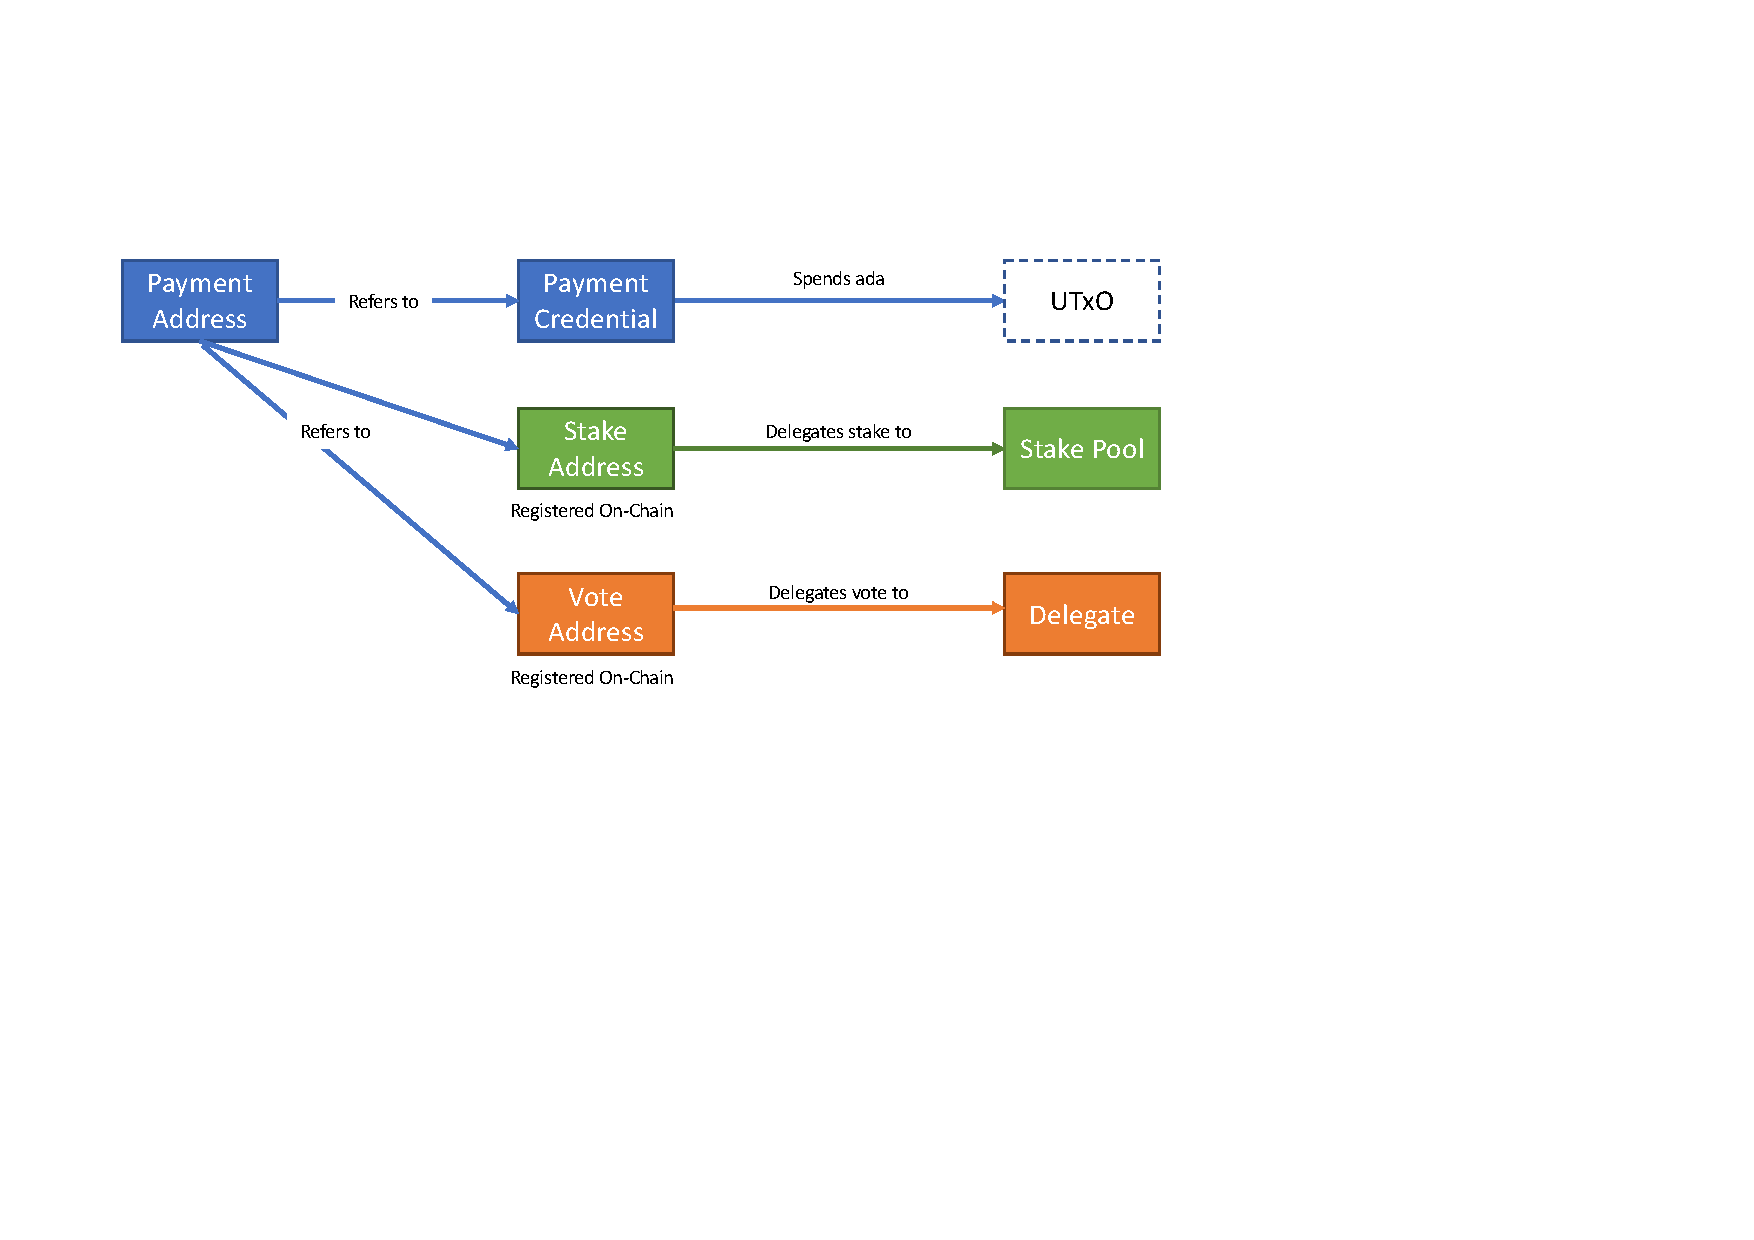
\includegraphics[trim=0 250 150 80,clip,width=\textwidth]{Indirection}
  \end{center}
  \caption{Relationship between payment addresses, payment credentials, vote addresses and stake addresses}
  \label{fig:indirection}
\end{figure*}

\subsubsection*{Payment, Stake and Vote Rights}

Figure~\ref{fig:indirection} outlines how payment addresses relate to payment credentials, stake addresses  and vote addresses.  Payment credentials are used to
authorise payments of any kind, including transacion fees.  Unspent ada is accumulated in UTxOs (Unspent Transaction Outputs).  These UTxOs may either be associated
with the payment address (so returning unspent ada to the user's account), or may be associated with some other address (so allowing ada to be transferred to other wallets,
including those owned by third parties.  If payment credentials are given to a third party, they will have full spending rights over the associated ada.  These rights cannot be
revoked without withdrawing all the associated ada. \khcomment{Not completely clear how the payment address is then removed - there's no on-chain registration.  Does it just become
useless and a target for GC?}
In Shelley, stake addresses are used to delegate block production rights.  They must be registered on chain before use.  They may be passed with the associated secret key to third parties
in order to allow them to delegate on behalf of the ada holder.  This may be useful to protect the original capital while allowing custodial delegation, for example.  Similarly,
the payment credentials may be protected by a hardware wallet, while the stake rights may be protected by software.  This may be more convenient where the hardware wallet is
held securely, for example.
In Voltaire, vote delegation is designed analogously to stake delegation.  It follows that vote rights may be passed on to the same or a different third party (or even retained), as required by the user,
and that voting rights may be asserted without needing the secret payment key.  Both stake and vote addresses may be independently de-registered at any time, in which case the associated delegation rights are immediately
revoked.  New addresses may then be created and assigned as required, and new delegations may be made.  This mechanism also provides protection against lost or stolen stake or vote keys.

\begin{figure*}[h]
  \begin{center}
  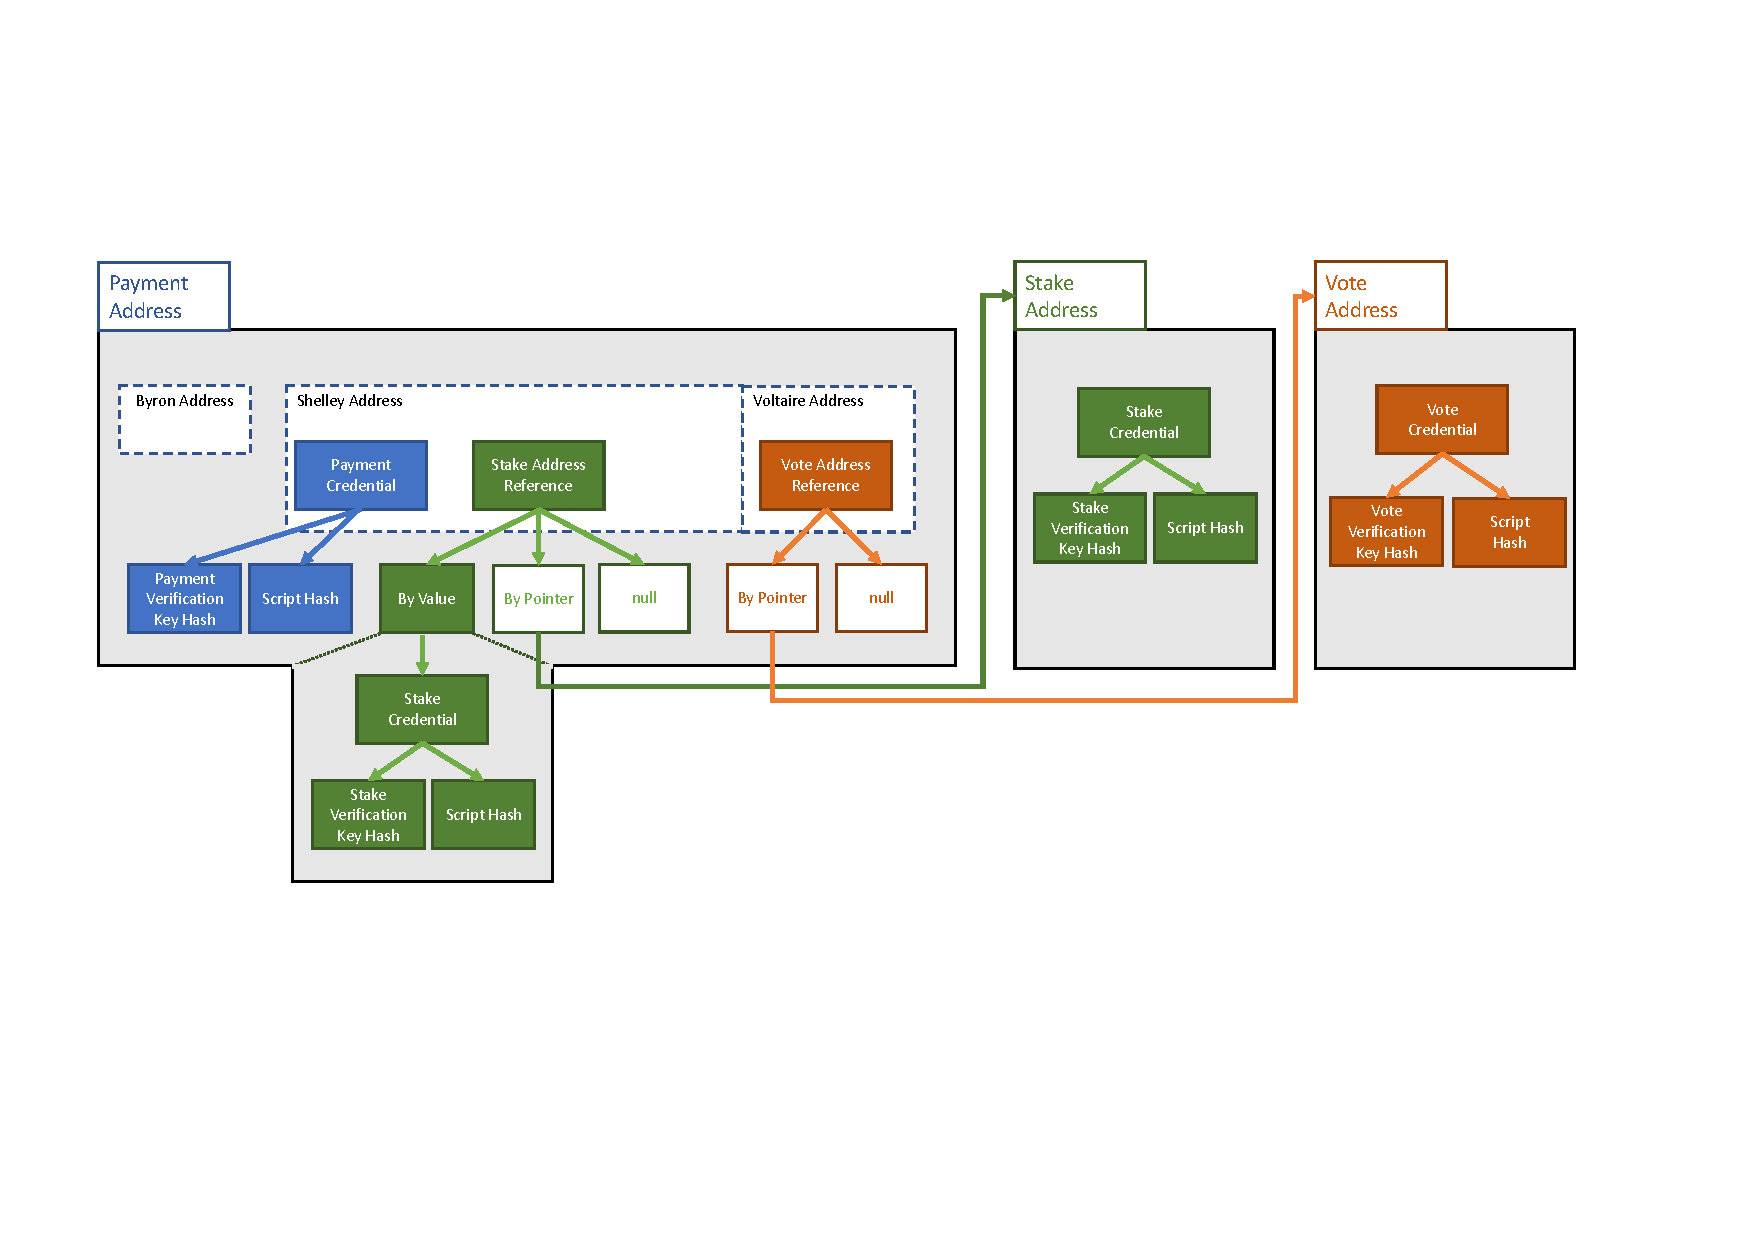
\includegraphics[trim=10 150 30 80,clip,width=\textwidth]{Address-Structure}
  \end{center}
  \caption{Payment Stake and Vote Address Structure}
  \label{fig:address-structure}
\end{figure*}

\subsubsection*{Revised Payment Address Structure}

The revised structure for payment addresses is shown in Figure~\ref{fig:address-structure} (this is adapted from the Shelley delegation design document~\cite{delegation-design}).
Payment addresses may be either Byron Addresses, Shelley Addresses or Voltaire Addresses.
\khcomment{There's apparently no on-chain registration for payment addresses.}
Voltaire addresses extend Shelley addresses by including a vote address reference in addition to the existing payment credential and stake address
reference fields.  Payment credentials may be either payment verification key hashes or script hashes.  Stake address references may be either
by value (in which case the stake credential is directly embedded in the address), by pointer to the registration transaction, or null (an efficient
form used where payment addresses do not need stake delegation rights).
Stake addresses refer to a stake credential that must either be a stake verification key hash or a script hash.
\khcomment{The Shelley address design looks over-complicated -- stake references could probably be collapsed to just pointers.}
Voltaire extends the Shelley address format by including vote address references.  These must be either by pointer to the registration transaction, or null (an efficient
form used where payment addresses do not need vote delegation rights).
\khcomment{I think the null form might not be used?  In which case we could avoid problems by eliminating it.  However, the vote address would then need either to be optional
or it would be necessary to always register the vote credentials with the payment address.}
Vote addresses refer to a vote credential that is must be a vote verification key hash.
\khcomment{The different levels seem a bit confusing.  An address is presumably a reference to the structure.  But embedded stake credentials won't have an address.  Credentials similarly
seem to always collapse down to the underlying structure (so may be naming artefects that do not really need to exist).}
\khcomment{Should script hashes be allowed as voting credentials?  I would imagine so.}
The same registration/de-registration concerns apply when pointers are used for vote address references as for stake address references (see ~\cite{delegation-design}).
Although these can be specified separately, enterprise addresses are expected to have both null stake address references and null vote address references.
\khcomment{A single null would do here for both kinds of address reference in an enterprise address, but that would be a bit harder to fit with the existing structure.}

\begin{figure*}[h]
  \begin{center}
  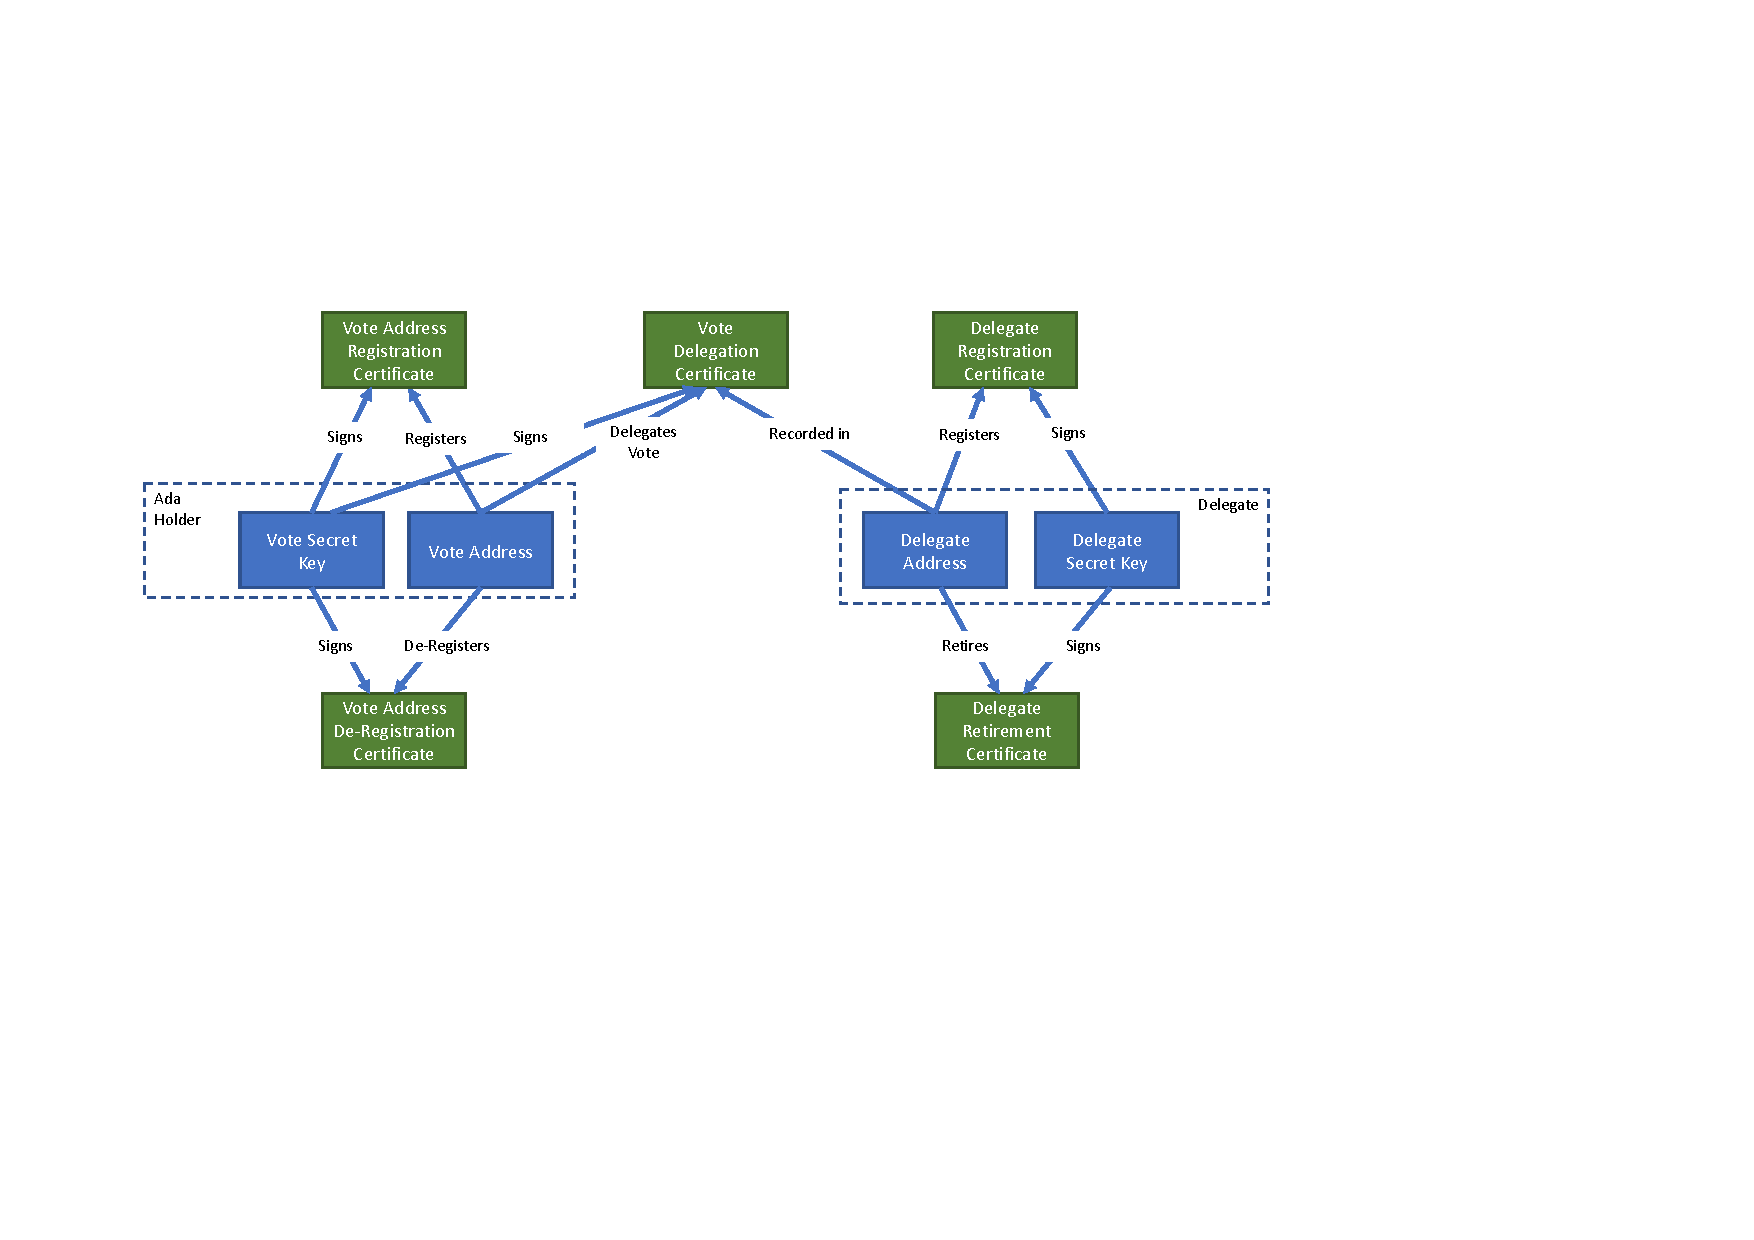
\includegraphics[trim=10 150 30 80,clip,width=\textwidth]{Relationships}
  \end{center}
  \caption{Relationships between vote addresses, keys and certificates}
  \label{fig:relationships}
\end{figure*}

\subsubsection*{Certificates and Registrations}

The Shelley design supports the following kinds of registration certificate to cover the registration/de-registration of stake addresses and stake pools on the blockchain:

\begin{itemize}
\item
Stake address registration certificate;
\item
Stake address de-registration certificate;
\item
Stake delegation certificate;
\item
Stake pool registration certificate;
\item
Stake pool retirement certificate;
\item
Stake pool operational key certificate.
\end{itemize}

The Voltaire design adds the following in an analogous way:

\begin{itemize}
\item
Vote address registration certificate;
\item
Vote address de-registration certificate;
\item
Vote delegation certificate;
\item
Delegate registration certificate;
\item
Delegate retirement certificate;
\end{itemize}



The relationships between these certificates and the vote address and vote keys is shown in Figure~\ref{fig:relationships}.
This is analogous to the design for stake addresses and certificates.
\khcomment{The actual relationships between keys, addresses and certificates are rather unclear in the stake delegation design document.  I think this is correct
but the original document might need to be fixed up...
It's not quite clear when things should be public keys and when they need to be addresses, or which things need actually to be included in the certificates.}
However, unlike the Shelley stake delegation design, the vote design does not need a cold/hot (KES) key structure, a VRF key, or an operational certificate.
\khcomment{I assume hot/cold isn't needed, since security is not directly affected, but I may be wrong?  VRF and operational certificates are certainly not needed.}

\subsubsection*{Certificate Precedence and Validity}

The blockchain specifies a strong and verifiabe temporal ordering on events.
Newer vote, vote delegation, and delegate certificates always override older ones.  Certificates remain in force until they are revoked or a newer certificate is issued,
whichever comes first.  Vote and delegate certificates may be revoked.  Vote delegations are not explicitly revoked, but are only valid when both the vote certificate
and delegate certificate are also in force.
Newer delegation certificates override older delegation certificates. This allows delegators to move from one stake pool to another.

\section{Ledger State Transition}
\label{sec:ledger-trans}

The entire state transformation of the ledger state caused by a valid transaction
can now be given as the combination of the UTxO transition and the delegation transitions.

Figure~\ref{fig:ts-types:ledger} defines the types for this transition.
The environment for this rule consists of:
\begin{itemize}
  \item The current slot.
  \item The transaction index within the current block.
  \item The protocol parameters.
  \item The accounting state.
\end{itemize}
The ledger state consists of:
\begin{itemize}
  \item The UTxO state.
  \item The delegation and pool states.
\end{itemize}

\begin{figure}[htb]
  \emph{Ledger environment}
  \begin{equation*}
    \LEnv =
    \left(
      \begin{array}{r@{~\in~}lr}
        \var{slot} & \Slot & \text{current slot}\\
        \var{txIx} & \Ix & \text{transaction index}\\
        \var{pp} & \PParams & \text{protocol parameters}\\
        \var{acnt} & \Acnt & \text{accounting state}
      \end{array}
    \right)
  \end{equation*}
  %
  \emph{Ledger state}
  \begin{equation*}
    \LState =
    \left(
      \begin{array}{r@{~\in~}lr}
        \var{utxoSt} & \UTxOState & \text{UTxO state}\\
        \var{dpstate} & \DPState & \text{delegation and pool state}\\
      \end{array}
    \right)
  \end{equation*}
  %
  \emph{Ledger transitions}
  \begin{equation*}
    \_ \vdash
    \var{\_} \trans{ledger}{\_} \var{\_}
    \subseteq \powerset (\LEnv \times \LState \times \Tx \times \LState)
  \end{equation*}
  \caption{Ledger transition-system types}
  \label{fig:ts-types:ledger}
\end{figure}

Figure~\ref{fig:ts-types:ledger} defines the ledger state transition.
It has a single rule, which first calls the $\mathsf{UTXOW}$ transition,
then calls the $\mathsf{DELEGS}$ transition.

\begin{figure}
  \begin{equation}
    \label{eq:ledger}
    \inference[ledger]
    {
      {
        \begin{array}{c}
          \var{slot} \\
          \var{txIx} \\
          \var{pp} \\
          \var{tx}\\
          \var{acnt}
        \end{array}
      }
      \vdash
      dpstate \trans{\hyperref[fig:rules:delegation-sequence]{delegs}}{
        \fun{txcerts}~\var{(\txbody{tx})}} dpstate'
      \\~\\
      (\var{dstate}, \var{pstate}) \leteq \var{dpstate} \\
      (\_, \_, \_, \_, \var{genDelegs}, \_) \leteq \var{dstate} \\
      (\var{poolParams}, \_, \_) \leteq \var{pstate} \\
      \\~\\
      {
        \begin{array}{c}
        \var{slot} \\
        \var{pp} \\
        \var{poolParams} \\
        \var{genDelegs} \\
        \end{array}
      }
      \vdash \var{utxoSt} \trans{\hyperref[fig:rules:utxow-shelley]{utxow}}{tx} \var{utxoSt'}
    }
    {
      \begin{array}{c}
        \var{slot} \\
        \var{txIx} \\
        \var{pp} \\
        \var{acnt}
      \end{array}
      \vdash
      \left(
        \begin{array}{ll}
          \var{utxoSt} \\
          \var{dpstate} \\
        \end{array}
      \right)
      \trans{ledger}{tx}
      \left(
        \begin{array}{ll}
          \varUpdate{utxoSt'} \\
          \varUpdate{dpstate'} \\
        \end{array}
      \right)
    }
  \end{equation}
  \caption{Ledger inference rule}
  \label{fig:rules:ledger}
\end{figure}

\clearpage

The transition system $\mathsf{LEDGER}$ in Figure~\ref{fig:rules:ledger} is iterated
in $\mathsf{LEDGERS}$ in order to process a list of transactions.

\begin{figure}[htb]
  \emph{Ledger Sequence transitions}
  \begin{equation*}
    \_ \vdash
    \var{\_} \trans{ledgers}{\_} \var{\_}
    \subseteq \powerset ((\Slot\times\PParams\times\Coin) \times \LState \times \seqof{\Tx} \times \LState)
  \end{equation*}
  \caption{Ledger Sequence transition-system types}
  \label{fig:ts-types:ledgers}
\end{figure}

\begin{figure}[hbt]
  \begin{equation}
    \label{eq:ledgers-base}
    \inference[Seq-ledger-base]
    { }
    {
      \begin{array}{r}
        \var{slot}\\
        \var{pp}\\
        \var{acnt}
      \end{array}
      \vdash \var{ls} \trans{ledgers}{\epsilon} \var{ls}
    }
  \end{equation}

  \nextdef

  \begin{equation}
    \label{eq:ledgers-induct}
    \inference[Seq-ledger-ind]
    {
      {
        \begin{array}{r}
          \var{slot}\\
          \var{pp}\\
          \var{acnt}
        \end{array}
      }
      \vdash
      \var{ls}
      \trans{ledgers}{\Gamma}
      \var{ls'}
      &
      {
        \begin{array}{r}
          \var{slot}\\
          \mathsf{len}~\Gamma\\
          \var{pp}\\
          \var{acnt}
        \end{array}
      }
      \vdash
        \var{ls'}
        \trans{\hyperref[fig:rules:ledger]{ledger}}{\var{tx}}
        \var{ls''}
    }
    {
      \begin{array}{r}
        \var{slot}\\
        \var{pp}\\
        \var{acnt}
      \end{array}
    \vdash
      \var{ls}
      \trans{ledgers}{\Gamma;~\var{tx}}
      \varUpdate{\var{ls''}}
    }
  \end{equation}
  \caption{Ledger sequence rules}
  \label{fig:rules:ledger-sequence}
\end{figure}

\section{Rewards and the Epoch Boundary}
\label{sec:epoch}

\newcommand{\UTxOEpState}{\type{UTxOEpState}}
\newcommand{\PlReapState}{\type{PlReapState}}
\newcommand{\NewPParamEnv}{\type{NewPParamEnv}}
\newcommand{\Snapshot}{\type{Snapshot}}
\newcommand{\Snapshots}{\type{Snapshots}}
\newcommand{\SnapshotEnv}{\type{SnapshotEnv}}
\newcommand{\SnapshotState}{\type{SnapshotState}}
\newcommand{\NewPParamState}{\type{NewPParamState}}
\newcommand{\EpochState}{\type{EpochState}}
\newcommand{\BlocksMade}{\type{BlocksMade}}
\newcommand{\Stake}{\type{Stake}}
\newcommand{\RewardUpdate}{\type{RewardUpdate}}

\newcommand{\obligation}[3]{\fun{obligation}~ \var{#1}~ \var{#2}~ \var{#3}}
\newcommand{\reward}[8]{\fun{reward}
  ~ \var{#1}~ \var{#2}~ \var{#3}~ \var{#4}~ \var{#5}~ \var{#6}~ \var{#7}~ \var{#8}}
\newcommand{\isActive}[4]{\fun{isActive}~ \var{#1}~ \var{#2}~ \var{#3}~ \var{#4}}
\newcommand{\activeStake}[5]{\fun{activeStake}~ \var{#1}~ \var{#2}~ \var{#3}~ \var{#4}~ \var{#5}}
\newcommand{\poolRefunds}[2]{\fun{poolRefunds}~ \var{#1}~ \var{#2}}
\newcommand{\poolStake}[3]{\fun{poolStake}~ \var{#1}~ \var{#2}~ \var{#3}}
\newcommand{\stakeDistr}[3]{\fun{stakeDistr}~ \var{#1}~ \var{#2}~ \var{#3}}
\newcommand{\lReward}[4]{\fun{r_{operator}}~ \var{#1}~ \var{#2}~ \var{#3}~ {#4}}
\newcommand{\mReward}[4]{\fun{r_{member}}~ \var{#1}~ \var{#2}~ \var{#3}~ {#4}}
\newcommand{\mkApparentPerformance}[4]{\fun{mkApparentPerformance}~\var{#1}~{#2}~\var{#3}~\var{#4}}
\newcommand{\createRUpd}[4]{\fun{createRUpd}~\var{#1}~\var{#2}~\var{#3}~\var{#4}}
\newcommand{\getIR}[1]{\fun{getIR}~\var{#1}}

This chapter introduces the epoch boundary transition system and the related reward calculation.

The transition system is defined in Section~\ref{sec:total-epoch},
and involves taking stake distribution snapshots
(Sections~\ref{sec:stake-dist-calc} and~\ref{sec:snapshots}),
retiring stake pools (Section~\ref{sec:pool-reap}),
and performing protocol updates (Section~\ref{sec:pparam-update}).
The reward calculation, defined in Sections~\ref{sec:reward-dist} and~\ref{sec:reward-calc},
distributes the leader election rewards.

\subsection{Overview of the Reward Calculation}
\label{sec:reward-overview}

The rewards for a given epoch $e_i$ involve the two epochs surrounding it.
In particular, the stake distribution will come from the previous epoch
and the rewards will be calculated in the following epoch.
More concretely:
\begin{enumerate}[(A)]%for small alpha-characters within brackets.
  \item A stake distribution snapshot is taken at the begining of epoch $e_{i-1}$.
  \item The randomness for leader election is fixed during epoch $e_{i-1}$
  \item Epoch $e_{i}$ begins.
  \item Epoch $e_{i}$ ends.
    A snapshot is taken of the stake pool performance during epoch $e_{i}$.
    A snapshot is also taken of the fee pot.
  \item The snapshots from (D) are stable and the reward calculation can begin.
  \item The reward calculation is finished and an update to the ledger state
    is ready to be applied.
  \item Rewards are given out.
\end{enumerate}

\usetikzlibrary{decorations.pathreplacing}
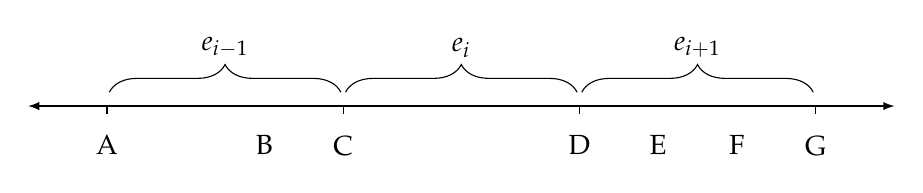
\begin{tikzpicture}
% axis
\draw[latex-latex] (0,0) -- (11,0) ;

% epoch braces
\draw [decorate,decoration={brace,amplitude=10pt} ,yshift=5pt] (1.03,0) -- (3.97,0)
  node [midway, above, yshift=9pt]{$e_{i-1}$};
\draw [decorate,decoration={brace,amplitude=10pt} ,yshift=5pt] (4.03,0) -- (6.97,0)
  node [midway, above, yshift=9pt]{$e_{i}$};
\draw [decorate,decoration={brace,amplitude=10pt} ,yshift=5pt] (7.03,0) -- (9.97,0)
  node [midway, above, yshift=9pt]{$e_{i+1}$};

% epoch boundaries
\foreach \x in  {1,4,7,10}
  \draw[shift={(\x,0)}] (0pt,0pt) -- (0pt,-3pt);

\node at (1,-0.5) {A};
\node at (3,-0.5) {B};
\node at (4,-0.5) {C};
\node at (7,-0.5) {D};
\node at (8,-0.5) {E};
\node at (9,-0.5) {F};
\node at (10,-0.5) {G};

\end{tikzpicture}

We must therefore store the last three stake distributions.
The mnemonic ``mark, set, go'' will be used to keep
track of the snapshots, where the label ``mark'' refers to the most recent snapshot,
and ``go'' refers to the snapshot that is ready to be used in the reward calculation.
In the above diagram, the snapshot taken at (A) is labeled ``mark'' during epoch $e_{i-1}$,
``set'' during epoch $e_i$ and ``go'' during epoch $e_{i+1}$. At (G) the snapshot
taken at (A) is no longer needed and will be discarded.

The two main transition systems in this section are:
\begin{itemize}
  \item The transition system named $\mathsf{EPOCH}$, which is defined in
    Section~\ref{sec:total-epoch}, covers what happens at the epoch boundary,
    such as at (A), (C), (D) and (G).
  \item The transition named $\mathsf{RUPD}$, which is defined in
    Section~\ref{sec:reward-update-trans}, covers the reward calculation that
    happens between (E) and (F).
\end{itemize}


\begin{note}
  Between time D and E we are concerned with chain growth and stability.
  Therefore this duration can be stated as 2k blocks (to state it in slots requires details about
  the particular version of the Ouroboros protocol). The duration between F and G is also 2k blocks.
  Between E and F a single honest block is enough to ensure a random nonce.
\end{note}

\subsection{Example Illustration of the Reward Cycle}
\label{sec:illustration-reward-cycle}

\definecolor{epochColor}{rgb} {1.00,0.50,0.00}
\definecolor{aliceColor}{rgb} {0.65,0.00,0.00}
\definecolor{bobColor}{rgb} {0.00,0.50,0.00}
\definecolor{bob2Color}{rgb} {0.00,0.95,0.00}
\definecolor{snapshot1}{rgb} {0.00,0.00,0.90}
\definecolor{snapshot2}{rgb} {0.00,0.60,0.90}

\begin{tikzpicture}

  % Axis
  \draw [thick] (-0.2,0) -- (13,0);
  \draw (0,-.2) -- (0, .2);
  \draw (3,-.2) -- (3, .2);
  \draw (6,-.2) -- (6, .2);
  \draw (9,-.2) -- (9, .2);
  \draw (12,-.2) -- (12, .2);
  \node[align=center, below, color=epochColor] at (1.5,0.5)
    {$e_1$};
  \node[align=center, below, color=epochColor] at (4.5,0.5)
    {$e_2$};
  \node[align=center, below, color=epochColor] at (7.5,0.5)
    {$e_3$};
  \node[align=center, below, color=epochColor] at (10.5,0.5)
    {$e_4$};

  % Alice
  % Alice's circle
  \draw [aliceColor, fill] (0,3) circle [radius=0.5];
  \node [white] at (0,3) {Alice};
  % Alice's delegation line
  \draw [->,thick, aliceColor] (0.4,2.65) to (2,0.05);
  \node [aliceColor] at (2.2,2) {delegate to Bob};

  % Bob
  % Bob's circle
  \draw [bobColor, fill] (0,-3) circle [radius=0.5];
  \node [white] at (0,-3) {Bob};
  % Bob's registration line
  \draw [->,thick, bobColor] (0.2,-2.50) to (1,-0.05);
  \node [align=left, below, bobColor] at (-0.5,-0.5) {initial pool \\ registration};
  % Bob's re-registration line
  \draw [->,thick, bob2Color] (0.45,-2.65) to (2.90,-0.05);
  \node [bob2Color] at (2,-2.8) {re-registration};
  % Bob's cached parameter change
  \draw [->,thick, bob2Color] (2.9,-0.2) to [out=280, in=180] (3,-2)
     to [out=0, in=290] (3.1,-0.2);

  % Alice time to re-delegate
  \draw [decorate, decoration = {brace, mirror, amplitude=10pt}, aliceColor, thick]
    (3.2,-0.2) to (5.9,-0.2);
  \node [align=center, below, aliceColor] at (5.1,-0.5)
    {Alice's opportunity \\ to re-delegate \\ before Bob's new \\ parameters};

  % Bob's blocks
  % epoch e3
  \draw [fill=bobColor,bobColor] (6.3,-.1) rectangle (6.5,-.3);
  \draw [fill=bobColor,bobColor] (6.7,-.1) rectangle (6.9,-.3);
  \draw [fill=bobColor,bobColor] (7.4,-.1) rectangle (7.6,-.3);
  \draw [fill=bobColor,bobColor] (8.4,-.1) rectangle (8.6,-.3);
  \draw [decorate, decoration = {brace, mirror, amplitude=10pt}, bobColor, thick]
    (6.2, -0.4) to (8.9,-0.4);
  \draw [->,thick, bobColor] (7.6, -0.8) to [out=315,in=200] (8.4, -1.2)
     to [] (9.6, -0.9);

  % epoch e4
  \draw [fill=bob2Color,bob2Color] (9.9,-.1) rectangle (10.1,-.3);
  \draw [fill=bob2Color,bob2Color] (10.4,-.1) rectangle (10.6,-.3);
  \draw [fill=bob2Color,bob2Color] (10.8,-.1) rectangle (11.0,-.3);
  \draw [decorate, decoration = {brace, mirror, amplitude=10pt}, bob2Color, thick]
    (9.7, -0.4) to (11.2,-0.4);
  \draw [->,thick, bob2Color] (10.6, -0.8) to [out=315,in=200] (11.4, -1.2)
     to [] (12.6, -0.9);

  % Snapshots
  \draw [->,thick, snapshot1] (3,0.3) to [out=90,in=150] (9,0.5)
     to [out=330,in=180] (10,-1) to [out=0,in=-135] (12,0) ;
   \node [snapshot1] at (2.7,1.2) {mark};
   \node [snapshot1] at (6,1.9) {set};
   \node [snapshot1] at (9,0.9) {go};

  \draw [->,thick, snapshot2] (6,0.3) to [out=90,in=150] (12,0.5)
     to [out=330,in=180] (13,-1);
   \node [snapshot2] at (5.7,1.2) {mark};
   \node [snapshot2] at (9,1.9) {set};
   \node [snapshot2] at (12,0.9) {go};
\end{tikzpicture}

Bob registers his stake pool in epoch $e_1$.
Alice delegates to Bob's stake pool in epoch $e_1$.
Just before the end of epoch $e_1$, Bob submits a stake pool re-registration,
changing his pool parameters. The change in parameters is not immediate,
as shown by the curved arrow around the epoch boundary.

A snapshot is taken on the $e_1$/$e_2$ boundary. It is labeled ``mark'' initially.
This snapshot includes Alice's delegation to Bob's pool, and Bob's pool parameters
and listed in the initial pool registration certificate.

If Alice changes her delegation choice any time during epoch $e_2$,
she will never be effected by Bob's change of parameters.

A new snapshot is taken on the $e_2$/$e_3$ boundary.
The previous (darker blue) snapshot is now labeled ``set'', and the new one labeled ``mark''.
The ``set'' snapshot is used for leader election in epoch $e_3$.

On the $e_3$/$e_4$ boundary, the darker blue snapshot is labeled ``go'' and
the lighter blue snapshot is labeled ``set''.
Bob's stake pool performance during epoch $e_3$ (he produced 4 blocks)
will be used with the darker blue snapshot for the rewards which will
be handed out at the beginning of epoch $e_5$.

\subsection{Helper Functions and Accounting Fields}
\label{sec:stake-dist-helpers}

Figure~\ref{fig:funcs:epoch-helper-rewards} defines four helper functions needed
throughout the rest of the section.

\begin{itemize}
  \item The function $\fun{obligation}$ calculates the the minimal amount of coin needed to
    pay out all deposit refunds.
  \item The function $\fun{poolStake}$ filters the stake distribution to one stake pool.
\end{itemize}


%%
%% Figure - Helper Functions for Epoch Rules
%%
\begin{figure}[htb]
  \emph{Total possible refunds}
  \begin{align*}
    & \fun{obligation} \in \PParams \to (\StakeCredential \mapsto \Coin)
    \to (\KeyHash_{pool}\mapsto\PoolParam) \to \Coin \\
    & \obligation{pp}{rewards}{poolParams} = \\
    & ~~~~~
    (\fun{keyDeposit}~\var{pp}) \cdot|\var{rewards}| +
    (\fun{poolDeposit}~\var{pp}) \cdot|\var{poolParams}| \\
  \end{align*}
  %
  \emph{Filter Stake to one Pool}
  \begin{align*}
      & \fun{poolStake} \in \KeyHash_{pool} \to (\KeyHash_{stake} \mapsto \KeyHash_{pool})
        \to \Stake \to \Stake \\
      & \poolStake{hk}{delegs}{stake} =
        \dom{(\var{delegs}\restrictrange\{hk\})\restrictdom\var{stake}}
  \end{align*}

  \caption{Helper Functions used in Rewards and Epoch Boundary}
  \label{fig:funcs:epoch-helper-rewards}
\end{figure}


The Figure~\ref{fig:defs:accounting} lists the accounting fields, denoted by $\Acnt$,
which will be used throughout this section. It consists of:
\begin{itemize}
  \item The value $\var{treasury}$ tracks the amount of coin currently stored in the treasury.
    Initially there will be no way to remove these funds.
  \item The value $\var{reserves}$ tracks the amount of coin currently stored in the reserves.
    This pot is used to pay rewards.
\end{itemize}
More will be said about the general accounting system in Section~\ref{sec:reward-calc}.

%%
%% Figure - Accounting fields
%%
\begin{figure}[htb]
  \emph{Accounting Fields}
  \begin{equation*}
    \Acnt =
    \left(
      \begin{array}{r@{~\in~}ll}
        \var{treasury} & \Coin & \text{treasury pot}\\
        \var{reserves} & \Coin & \text{reserve pot}\\
      \end{array}
    \right)
  \end{equation*}
  %
  \caption{Accounting fields}
  \label{fig:defs:accounting}
\end{figure}


\subsection{Stake Distribution Calculation}
\label{sec:stake-dist-calc}

This section defines the stake distribution calculations.
Figure~\ref{fig:epoch-defs} introduces three new derived types:
\begin{itemize}
  \item $\type{BlocksMade}$ represents the number of blocks each stake pool produced
    during an epoch.
  \item $\type{Stake}$ represents the amount of stake (in $\type{Coin}$) controlled by each
    stake pool.
\end{itemize}

%%
%% Figure - Epoch Abstract Types
%%
\begin{figure}[htb]
  \emph{Derived types}
  %
  \begin{equation*}
    \begin{array}{r@{~\in~}l@{\qquad=\qquad}lr}
      \var{blocks}
      & \BlocksMade
      & \KeyHash_{pool} \mapsto \N
      & \text{blocks made by stake pools} \\
      \var{stake}
      & \Stake
      & \Credential \mapsto \Coin
      & \text{stake} \\
    \end{array}
  \end{equation*}
  \caption{Epoch definitions}
  \label{fig:epoch-defs}
\end{figure}

The stake distribution calculation is given in Figure~\ref{fig:functions:stake-distribution}.

\begin{itemize}
\item $\fun{aggregate_{+}}$ takes a relation on $A\times B$, where $B$ is any
  monoid $(B,+,e)$ and returns a map from each $a\in A$ to the ``sum'' (using
  the monoidal $+$ operation) of all $b\in B$ such that $(a, b)\in A\times B$.
\item $\fun{stakeDistr}$ uses the $\fun{aggregate_{+}}$ function and several relations to
    compute the stake distribution, mapping each hashkey to the total coin under its control.
    Keys that are not both registered and delegated are filtered out.
    The relation passed to $\fun{aggregate_{+}}$ is made up of:
    \begin{itemize}
      \item $\fun{stakeCred_b}^{-1}$, relating credentials to (base) addresses
      \item $\left(\fun{addrPtr}\circ\var{ptr}\right)^{-1}$, relating credentials to (pointer)
        addresses
      \item $\range{utxo}$, relating addresses to coins
      \item $\fun{stakeCred_r}^{-1}\circ\var{rewards}$, relating (reward) addresses to coins
    \end{itemize}
    The notation for relations is explained in Section~\ref{sec:notation-shelley}.
\end{itemize}

%%
%% Figure Functions for Stake Distribution
%%
\begin{figure}[htb]
  \emph{Aggregation (for a monoid B)}
  %
  \begin{align*}
      & \fun{aggregate_{+}} \in \powerset{(A \times B)} \to (A\mapsto B) \\
      & \fun{aggregate_{+}}~\var{R} = \left\{a\mapsto \sum_{(a,b)\in\var{R}}b
          ~\mid~a\in\dom\var{R}\right\} \\
  \end{align*}
  %
  \emph{Stake Distribution (using functions and maps as relations)}
  %
  \begin{align*}
      & \fun{stakeDistr} \in \UTxO \to \DState \to \PState \to \Snapshot \\
      & \fun{stakeDistr}~{utxo}~{dstate}~{pstate} = \\
      & ~~~~ \big((\dom{\var{activeDelegs}})
      \restrictdom\left(\fun{aggregate_{+}}~\var{stakeRelation}\right),
    ~\var{delegations},~\var{poolParams}\big)\\
      & \where \\
      & ~~~~ (~\var{rewards},~\var{delegations},~\var{ptrs},~\wcard,~\wcard,~\wcard)
        = \var{dstate} \\
      & ~~~~ (~\var{poolParams},~\wcard,~\wcard) = \var{pstate} \\
      & ~~~~ \var{stakeRelation} = \left(
        \left(\fun{stakeCred_b}^{-1}\cup\left(\fun{addrPtr}\circ\var{ptr}\right)^{-1}\right)
        \circ\left(\range{\var{utxo}}\right)
        \right)
        \cup \var{rewards} \\
      & ~~~~ \var{activeDelegs} =
               (\dom{rewards}) \restrictdom \var{delegations} \restrictrange (\dom{poolParams}) \\
  \end{align*}

  \caption{Stake Distribution Function}
  \label{fig:functions:stake-distribution}
\end{figure}

\clearpage

\subsection{Snapshot Transition}
\label{sec:snapshots}

The state transition types for stake distribution snapshots are given in
Figure~\ref{fig:ts-types:snapshot}.
Each snapshot consists of:
\begin{itemize}
  \item $\var{stake}$, a stake distribution, which is defined in
    Figure~\ref{fig:epoch-defs} as a mapping of credentials to coin.
  \item $\var{delegations}$, a delegation map, mapping credentials to stake pools.
  \item $\var{poolParameters}$, storing the pool parameters of each stake pool.
\end{itemize}

The type $\type{\Snapshots}$ contains the
information needing to be saved on the epoch boundary:
\begin{itemize}
  \item $\var{pstake_{mark}}$, $\var{pstake_{set}}$ and $\var{pstake_{go}}$ are the three
    snapshots as explained in Section~\ref{sec:reward-overview}.
  \item $\var{feeSS}$ stores the fees which are added to the reward pot during
    the next reward update calculation, which is then subtracted from the fee pot
    on the epoch boundary.
\end{itemize}

%%
%% Figure - Snapshots Defs
%%
\begin{figure}[htb]
  \emph{Snapshots}
  \begin{equation*}
    \Snapshot =
    \left(
      \begin{array}{r@{~\in~}ll}
        \var{stake} & \Stake & \text{stake distribution}\\
        \var{delegations} & \Credential\mapsto\KeyHash_{pool}
                          & \text{stake delegations}\\
        \var{poolParameters} & \KeyHash_{pool} \mapsto \PoolParam & \text{pool parameters }\\
      \end{array}
    \right)
  \end{equation*}

  \begin{equation*}
    \Snapshots =
    \left(
      \begin{array}{r@{~\in~}ll}
        \var{pstake_{mark}} & \Snapshot & \text{newest stake}\\
        \var{pstake_{set}}  & \Snapshot & \text{middle stake}\\
        \var{pstake_{go}}   & \Snapshot & \text{oldest stake}\\
        \var{feeSS} & \Coin & \text{fee snapshot}\\
      \end{array}
    \right)
  \end{equation*}
  %
  \emph{Snapshot transitions}
  \begin{equation*}
    \_ \vdash
    \var{\_} \trans{snap}{} \var{\_}
    \subseteq \powerset (\LState \times \Snapshots \times \Snapshots)
  \end{equation*}
  %
  \caption{Snapshot transition-system types}
  \label{fig:ts-types:snapshot}
\end{figure}

The snapshot transition rule is given in Figure~\ref{fig:rules:snapshot}.
This transition has no preconditions and results in the following state change:

\begin{itemize}
  \item The oldest snapshot is replaced with the penultimate one.
  \item The penultimate snapshot is replaced with the newest one.
  \item The newest snapshot is replaced with one just calculated.
  \item The current fees pot is stored in $\var{feeSS}$. Note that this value will not
    change during the epoch, unlike the $\var{fees}$ value in the UTxO state.
\end{itemize}

%%
%% Figure - Snapshot Rule
%%
\begin{figure}[htb]
  \begin{equation}\label{eq:snapshot}
    \inference[Snapshot]
    {
      {
      \begin{array}{r@{~\leteq~}l}
        ((\var{utxo},~\wcard,\var{fees},~\wcard),~(\var{dstate},~\var{pstate})) & \var{lstate} \\
        \var{stake} & \stakeDistr{utxo}{dstate}{pstate} \\
      \end{array}
      }
    }
    {
      \begin{array}{r}
        \var{lstate} \\
      \end{array}
      \vdash
      \left(
        \begin{array}{r}
          \var{pstake_{mark}}\\
          \var{pstake_{set}}\\
          \var{pstake_{go}}\\
          \var{feeSS} \\
        \end{array}
      \right)
      \trans{snap}{}
      \left(
        \begin{array}{r}
          \varUpdate{\var{stake}} \\
          \varUpdate{\var{pstake_{mark}}} \\
          \varUpdate{\var{pstake_{set}}} \\
          \varUpdate{\var{fees}} \\
        \end{array}
      \right)
    }
  \end{equation}
  \caption{Snapshot Inference Rule}
  \label{fig:rules:snapshot}
\end{figure}

\clearpage

\subsection{Pool Reaping Transition}
\label{sec:pool-reap}

Figure~\ref{fig:ts-types:pool-reap} defines the types for the pool reap transition,
which is responsible for removing pools slated for retirement in the given epoch.

%%
%% Figure - Pool Reap Defs
%%
\begin{figure}[htb]
  \emph{Pool Reap State}
  \begin{equation*}
    \PlReapState =
    \left(
      \begin{array}{r@{~\in~}ll}
        \var{utxoSt} & \UTxOState & \text{utxo state}\\
        \var{acnt} & \Acnt & \text{accounting}\\
        \var{dstate} & \DState & \text{delegation state}\\
        \var{pstate} & \PState & \text{pool state}\\
      \end{array}
    \right)
  \end{equation*}
  %
  \emph{Pool Reap transitions}
  \begin{equation*}
    \_ \vdash \_ \trans{poolreap}{\_} \_ \in
    \powerset (\PParams \times \PlReapState \times \Epoch \times \PlReapState)
  \end{equation*}
  %
  \caption{Pool Reap Transition}
  \label{fig:ts-types:pool-reap}
\end{figure}


The pool-reap transition rule is given in Figure~\ref{fig:rules:pool-reap}.
This transition has no preconditions and results in the following state change:

\begin{itemize}
  \item For each retiring pool, the refund for the pool registration deposit is added to the
    pool's registered reward account, provided the reward account is still registered.
  \item The sum of all the refunds attached to unregistered reward accounts are added to the
    treasury.
  \item The deposit pool is reduced by the amount of claimed and unclaimed refunds.
  \item Any delegation to a retiring pool is removed.
  \item Each retiring pool is removed from all four maps in the pool state.
\end{itemize}

%%
%% Figure - Pool Reap Rule
%%
\begin{figure}[htb]
  \begin{equation}\label{eq:pool-reap}
    \inference[Pool-Reap]
    {
      {
      \begin{array}{r@{~\leteq~}l}
        \var{retired} & \dom{(\var{retiring}^{-1}~\var{e})} \\
        \var{pr} & \left\{
                   \var{hk}\mapsto(\fun{poolDeposit}~\var{pp})
                     \mid
                     \var{hk}\in\var{retired}
                   \right\}\\
        \var{rewardAcnts}
                 & \{\var{hk}\mapsto \fun{poolRAcnt}~\var{pool} \mid
                   \var{hk}\mapsto\var{pool} \in \var{retired}\restrictdom\var{poolParams} \} \\
        \var{rewardAcnts'} & \left\{
                        a \mapsto c
                        \mathrel{\Bigg|}
                        \begin{array}{r@{~\in~}l}
                          \var{hk} \mapsto c & \var{pr}, \\
                          \var{hk}\mapsto\var{a} & \var{rewardAcnts} \\
                        \end{array}
                      \right\} \\
        \var{refunds} & \dom{rewards}\restrictdom\var{rewardAcnts'} \\
        \var{mRefunds} & \dom{rewards}\subtractdom\var{rewardAcnts'} \\
        \var{refunded} & \sum\limits_{\wcard\mapsto c\in\var{refunds}} c \\
        \var{unclaimed} & \sum\limits_{\wcard\mapsto c\in\var{mRefunds}} c \\
      \end{array}
      }
    }
    {
      \var{pp}
      \vdash
      \left(
        \begin{array}{r}
          \var{utxo} \\
          \var{deposited} \\
          \var{fees} \\
          \var{ppup} \\
          ~ \\
          \var{treasury} \\
          \var{reserves} \\
          ~ \\
          \var{rewards} \\
          \var{delegations} \\
          \var{ptrs} \\
          \var{genDelegs} \\
          \var{fGenDelegs} \\
          \var{i_{rwd}} \\
          ~ \\
          \var{poolParams} \\
          \var{fPoolParams} \\
          \var{retiring} \\
        \end{array}
      \right)
      \trans{poolreap}{e}
      \left(
        \begin{array}{rcl}
          \var{utxo} \\
          \varUpdate{\var{deposited}}
          & \varUpdate{-}
          & \varUpdate{(\var{unclaimed} + \var{refunded})} \\
          \var{fees} \\
          \var{ppup} \\
          ~ \\
          \varUpdate{\var{treasury}} & \varUpdate{+} & \varUpdate{\var{unclaimed}} \\
          \var{reserves} \\
          ~ \\
          \varUpdate{\var{rewards}} & \varUpdate{\unionoverridePlus} & \varUpdate{\var{refunds}} \\
          \varUpdate{\var{delegations}} & \varUpdate{\subtractrange} & \varUpdate{\var{retired}} \\
          \var{ptrs} \\
          \var{genDelegs} \\
          \var{fGenDelegs} \\
          \var{i_{rwd}}\\
          ~ \\
          \varUpdate{\var{retired}} & \varUpdate{\subtractdom} & \varUpdate{\var{poolParams}} \\
          \varUpdate{\var{retired}} & \varUpdate{\subtractdom} & \varUpdate{\var{fPoolParams}} \\
          \varUpdate{\var{retired}} & \varUpdate{\subtractdom} & \varUpdate{\var{retiring}} \\
        \end{array}
      \right)
    }
  \end{equation}
  \caption{Pool Reap Inference Rule}
  \label{fig:rules:pool-reap}
\end{figure}

\clearpage

\subsection{Protocol Parameters Update Transition}
\label{sec:pparam-update}

Finally, reaching the epoch boundary may trigger a change in the protocol parameters.
The protocol parameters environment consists of the delegation and pool states,
and the signal is an optional new collection of protocol parameters
The state change is a change of the $\UTxOState$, the $\Acnt$ states and the current $\PParams$.
The type of this state transition is given in Figure~\ref{fig:ts-types:new-proto-param}.

%%
%% Figure - New Proto Param Defs
%%
\begin{figure}[htb]
  \emph{New Proto Param environment}
  \begin{equation*}
    \NewPParamEnv =
    \left(
      \begin{array}{r@{~\in~}ll}
        \var{dstate} & \DState & \text{delegation state}\\
        \var{pstate} & \PState & \text{pool state}\\
      \end{array}
    \right)
  \end{equation*}
  %
  \emph{New Proto Param States}
  \begin{equation*}
    \NewPParamState =
    \left(
      \begin{array}{r@{~\in~}ll}
        \var{utxoSt} & \UTxOState & \text{utxo state}\\
        \var{acnt} & \Acnt & \text{accounting}\\
        \var{pp} & \PParams & \text{current protocol parameters}\\
      \end{array}
    \right)
  \end{equation*}
  %
  \emph{New Proto Param transitions}
  \begin{equation*}
    \_ \vdash
    \var{\_} \trans{newpp}{\_} \var{\_}
    \subseteq \powerset (\NewPParamEnv \times \NewPParamState \times \PParams^? \times \NewPParamState)
  \end{equation*}
  %
  \caption{New Proto Param transition-system types}
  \label{fig:ts-types:new-proto-param}
  %
  \emph{Helper Functions}
  \begin{align*}
      & \fun{updatePpup} \in \UTxOState \to \PParams \to \UTxOState\\
      & \fun{updatePpup}~\var{utxoSt}~\var{pp} =
      \begin{cases}
        (\var{utxo},\var{deposited},\var{fees},(\var{fpup},~\emptyset))
        &
        \var{canFollow}
        \\
        (\var{utxo},\var{deposited},\var{fees},(\emptyset,~\emptyset))
        &
        \text{otherwise} \\
      \end{cases}\\
      & ~~~\where \\
      & ~~~~~~~\var{canFollow} =
        \forall\var{ps}\in\range{pup},~
        \var{pv}\mapsto\var{v}\in\var{ps}\implies\fun{pvCanFollow}~(\fun{pv}~\var{pp})~\var{v}
        \\
      & ~~~~~~~(\var{utxo},\var{deposited},\var{fees},(\var{pup},~\var{fpup})) = \var{utxoSt} \\
  \end{align*}
\end{figure}


Figure~\ref{fig:rules:new-proto-param} defines the new protocol parameter transition.
The transition has two rules, depending on whether or not the new protocol parameters
meet some requirements.
In particular, we require that the new parameters would not incur a debt of the system that
can not be covered by the reserves, and that the max block size is greater than the sum of the
max transaction size and the max header size.
If the requirements are met, the new protocol parameters are accepted, the proposal is reset,
and the reserves are adjusted to account for changes in the deposits.
Otherwise, the only change is that the proposal is reset.

The $\mathsf{NEWPP}$ rule also cleans up the protocol parameter update proposals,
by calling $\fun{updatePpup}$ on the UTxO state.
The $\fun{updatePpup}$ sets the protocol parameter updates to the future protocol
parameter updates provided the protocol versions all can follow from the
version given in the protocol parameters, or the emptyset otherwise.
In any case, the future protocol parameters update proposals are set to the empty set.
If new protocol parameters are being adopted, then these is the value given to
$\fun{updatePpup}$, otherwise the old parameters are given.

Regarding adjusting the reserves for changes in the deposits, one of three things happens:

\begin{itemize}
  \item If the new protocol parameters mean that \textbf{fewer} funds are required in the
    deposit pot to cover all possible refunds, then the excess is moved to the reserves.

  \item If the new protocol parameters mean that \textbf{more} funds are required in the
    deposit pot to cover all possible refunds and the difference is \textbf{less} than
    the reserve pot, then funds are moved from the reserve pot to cover the difference.

  \item If the new protocol parameters mean that \textbf{more} funds are required in the
    deposit pot to cover all possible refunds and the difference is \textbf{more} than
    the reserve pot, then Rule~\ref{eq:new-pc-denied} meets the precondition and the
    only change of state is that the update proposals are reset.
\end{itemize}

Note that here, unlike most of the inference rules in this document,
the $\var{utxoSt'}$ and the $\var{acnt'}$ do not come from valid UTxO or
accounts transitions in the antecedent. We simply define the consequent
transition using these directly (instead of listing all the fields in both
states in the consequent transition). It is done this way here
for ease of reading.

%%
%% Figure - New Proto Param Rule
%%
\begin{figure}[htb]
  \begin{equation}\label{eq:new-pc-accepted}
    \hspace{-0.3cm}
    \inference[New-Proto-Param-Accept]
    {
      \var{pp_{new}}\neq\Nothing \\~\\
      {\begin{array}{rcl}
         (\var{utxo},~\var{deposited},~\var{fees},~\var{ppup}) & \leteq & \var{utxoSt} \\
         \var{(\var{rewards},~\wcard,~\wcard,~\wcard,~\wcard,~\var{i_{rwd}})} &
         \leteq & \var{dstate}\\
         \var{(\var{poolParams},~\wcard,~\wcard)} & \leteq & \var{pstate}\\
         \var{oblg_{cur}} & \leteq & \obligation{pp}{rewards}{poolParams} \\
         \var{oblg_{new}} & \leteq & \obligation{pp_{new}}{rewards}{poolParams} \\
         \var{diff} & \leteq & \var{oblg_{cur}} - \var{oblg_{new}}\\
      \end{array}}
      \\~\\~\\
      \var{oblg_{cur}} = \var{deposited} \\
      \var{reserves} + \var{diff} \geq \sum\limits_{\wcard\mapsto\var{val}\in\var{i_{rwd}}} val \\
      \fun{maxTxSize}~\var{pp_{new}} + \fun{maxHeaderSize}~\var{pp_{new}} <
        \fun{maxBlockSize}~\var{pp_{new}}
      \\~\\
        \var{utxoSt'} \leteq
        \left(\var{utxo},~\varUpdate{oblg_{new}},~\var{fees},~\var{ppup}\right)
      \\
      \var{utxoSt''} \leteq \fun{updatePpup}~\var{utxoSt'}~\var{pp_{new}}
      \\~\\
      (\var{treasury},~\var{reserves})\leteq \var{acnt} \\
      \var{acnt'} \leteq (\var{treasury},~\varUpdate{reserves + diff}) \\
    }
    {
      \begin{array}{l}
        \var{dstate}\\
        \var{pstate}\\
      \end{array}
      \vdash
      \left(
        \begin{array}{r}
          \var{utxoSt} \\
          \var{acnt} \\
          \var{pp}
        \end{array}
      \right)
      \trans{newpp}{\var{pp_{new}}}
      \left(
        \begin{array}{rcl}
          \varUpdate{utxoSt''}\\
          \varUpdate{acnt'} \\
          \varUpdate{\var{pp_{new}}} \\
        \end{array}
      \right)
    }
  \end{equation}

  \nextdef

  \begin{equation}\label{eq:new-pc-denied}
    \inference[New-Proto-Param-Denied]
    {
      \left({\begin{array}{c}
            \var{pp_{new}}=\Nothing \\
        \lor \\
        \var{reserves} + \var{diff} < \sum\limits_{\wcard\mapsto\var{val}\in\var{i_{rwd}}} val\\
        \lor \\
        \fun{maxTxSize}~\var{pp_{new}} + \fun{maxHeaderSize}~\var{pp_{new}} \geq
          \fun{maxBlockSize}~\var{pp_{new}}
      \end{array}}\right)
      \\~\\~\\
      {\begin{array}{rcl}
          \var{(\var{rewards},~\wcard,~\wcard,~\wcard,~\wcard,~\var{i_{rwd}})} &
          \leteq & \var{dstate}\\
         \var{(\var{poolParams},~\wcard,~\wcard)} & \leteq & \var{pstate}\\
          \var{oblg_{cur}} & \leteq & \obligation{pp}{rewards}{poolParams} \\
          \var{oblg_{new}} & \leteq & \obligation{pp_{new}}{rewards}{poolParams} \\
         \var{diff} & \leteq & \var{oblg_{cur}} - \var{oblg_{new}}
      \end{array}}
      \\~\\~\\
      \var{utxoSt'} \leteq \fun{updatePpup}~\var{utxoSt}~\var{pp} \\
    }
    {
      \begin{array}{l}
        \var{dstate}\\
        \var{pstate}\\
      \end{array}
      \vdash
      \left(
        \begin{array}{r}
          \var{utxoSt} \\
          \var{acnt} \\
          \var{pp}
        \end{array}
      \right)
      \trans{newpp}{\var{pp_{new}}}
      \left(
        \begin{array}{rcl}
          \varUpdate{utxoSt'}\\
          \var{acnt} \\
          \var{pp}
        \end{array}
      \right)
    }
  \end{equation}
  \caption{New Proto Param Inference Rule}
  \label{fig:rules:new-proto-param}
\end{figure}

\clearpage

\subsection{Complete Epoch Boundary Transition}
\label{sec:total-epoch}

Finally, it is possible to define the complete epoch boundary transition type,
which is defined in Figure~\ref{fig:ts-types:epoch}.
The transition has no evironment.
The state is made up of the the accounting state, the snapshots, the ledger state and the
protocol parameters.
The transition uses a helper function $\fun{votedValue}$ which returns
the consensus value of update proposals in the event that consensus is met.
\textbf{Note that} $\fun{votedValue}$
\textbf{is only well-defined if } $\var{quorum}$
\textbf{is greater than half the number of core nodes, i.e.}
$\Quorum > |\var{genDelegs}|/2$ \textbf{.}

%%
%% Figure - Epoch Defs
%%
\begin{figure}[htb]
  \emph{Epoch States}
  \begin{equation*}
    \EpochState =
    \left(
      \begin{array}{r@{~\in~}ll}
        \var{acnt} & \Acnt & \text{accounting}\\
        \var{ss} & \Snapshots & \text{snapshots}\\
        \var{ls} & \LState & \text{ledger state}\\
        \var{prevPp} & \PParams & \text{previous protocol parameters}\\
        \var{pp} & \PParams & \text{protocol parameters}\\
      \end{array}
    \right)
  \end{equation*}
  %
  \emph{Epoch transitions}
  \begin{equation*}
    \vdash
    \var{\_} \trans{epoch}{\_} \var{\_}
    \subseteq \powerset (\EpochState \times \Epoch \times \EpochState)
  \end{equation*}
  %
  \emph{Accessor Functions}
  \begin{equation*}
    \begin{array}{r@{~\in~}lr}
      \fun{getIR} & \EpochState \to (\StakeCredential \mapsto \Coin)
                  & \text{get instantaneous rewards} \\
    \end{array}
  \end{equation*}
  %
  \emph{Helper Functions}
  \begin{align*}
      & \fun{votedValue} \in (\KeyHashGen\mapsto\PParamsUpdate) \to \PParams \to \N \to \PParamsUpdate^?\\
      & \fun{votedValue}~\var{pup}~\var{pp}~\var{quorum} =
      \begin{cases}
        \var{pp}\unionoverrideRight\var{p}
          & \exists! p\in\range{pup}~(|pup\restrictrange p|\geq \var{quorum}) \\
        \Nothing & \text{otherwise} \\
      \end{cases}
  \end{align*}
  %
  \caption{Epoch transition-system types}
  \label{fig:ts-types:epoch}
\end{figure}


The epoch transition rule calls $\mathsf{SNAP}$, $\mathsf{POOLREAP}$ and $\mathsf{NEWPP}$
in sequence. It also stores the previous protocol parameters in $\var{prevPp}$.
The previous protocol parameters will be used for the reward calculation in the upcoming epoch,
note that they correspond to the epoch for which the rewards are being calculated.
Additionally, this transition also adopts the pool parameters $\var{fPoolParams}$
corresponding to the pool re-registration certificates which we submitted late in the ending epoch.
The ordering of these rules is important.
The stake pools which will be updated by $\var{fPoolParams}$ or
reaped during the $\mathsf{POOLREAP}$ transition must still be a
part of the new snapshot, and so $\mathsf{SNAP}$ must occur before these two actions.
Moreover, $\mathsf{SNAP}$ sets the deposit pot equal to current obligation,
which is a property that is preserved by $\mathsf{POOLREAP}$ and which
is necessary for the preservation of Ada property in the $ \mathsf{NEWPP}$ transition.

%%
%% Figure - Epoch Rule
%%
\begin{figure}[htb]
  \begin{equation}\label{eq:epoch}
    \inference[Epoch]
    {
      {
        \begin{array}{r}
          \var{lstate} \\
        \end{array}
      }
      \vdash
      { \var{ss} }
      \trans{\hyperref[fig:rules:snapshot]{snap}}{}
      { \var{ss'} }
      \\~\\
      (\var{utxoSt},~(\var{dstate},~\var{pstate}))\leteq\var{ls} \\
      (\var{poolParams},~\var{fPoolParams},~\var{retiring})\leteq\var{pstate}
      \\
      \var{pstate'}\leteq(\var{poolParams}\unionoverrideRight\var{fPoolParams},
      ~\emptyset,~\var{retiring})
      \\~\\~\\
      \var{pp}
      \vdash
      \left(
        {
          \begin{array}{r}
            \var{utxoSt} \\
            \var{acnt} \\
            \var{dstate} \\
            \var{pstate'} \\
          \end{array}
        }
      \right)
      \trans{\hyperref[fig:rules:pool-reap]{poolreap}}{e}
      \left(
      {
        \begin{array}{rcl}
            \var{utxoSt'} \\
            \var{acnt'} \\
            \var{dstate'} \\
            \var{pstate''} \\
        \end{array}
      }
      \right)
      \\~\\~\\
      \var{(\wcard,~\wcard,~\wcard,~(\var{pup},\wcard))}\leteq\var{utxoSt'}\\
      \var{pp_{new}}\leteq\fun{votedValue}~\var{pup}~\var{pp}~\Quorum\\
      {
        \begin{array}{r}
          \var{dstate'}\\
          \var{pstate''}\\
        \end{array}
      }
      \vdash
      \left(
        {
          \begin{array}{r}
            \var{utxoSt'} \\
            \var{acnt'} \\
            \var{pp}\\
          \end{array}
        }
      \right)
      \trans{\hyperref[fig:rules:new-proto-param]{newpp}}{\var{pp_{new}}}
      \left(
      {
        \begin{array}{rcl}
            \var{utxoSt''} \\
            \var{acnt''} \\
            \var{pp'}\\
        \end{array}
      }
      \right)
      \\~\\~\\
      \var{ls}' \leteq (\var{utxoSt}'',~(\var{dstate}',~\var{pstate}''))
    }
    {
      \vdash
      \left(
      \begin{array}{r}
        \var{acnt} \\
        \var{ss} \\
        \var{ls} \\
        \var{prevPp} \\
        \var{pp} \\
      \end{array}
      \right)
      \trans{epoch}{e}
      \left(
      \begin{array}{rcl}
        \varUpdate{\var{acnt''}} \\
        \varUpdate{\var{ss'}} \\
        \varUpdate{\var{ls'}} \\
        \varUpdate{\var{pp}} \\
        \varUpdate{\var{pp'}} \\
      \end{array}
      \right)
    }
  \end{equation}
  \caption{Epoch Inference Rule}
  \label{fig:rules:epoch}
\end{figure}

\clearpage

\subsection{Rewards Distribution Calculation}
\label{sec:reward-dist}

This section defines the reward calculation for the proof of stake leader election.
Figure~\ref{fig:functions:rewards} defines the pool reward as described in section
5.5.2 of~\cite{delegation_design}.

\begin{itemize}
  \item The function $\fun{maxPool}$ gives the maximum reward a stake pool can receive in an epoch.
    This is a fraction of the total available rewards for the epoch.
    The result depends on the pool's relative stake, the pool's pledge and the following
    protocol parameters:
    \begin{itemize}
      \item $\var{a_0}$, the leader-stake influence
      \item $n_{opt}$, the optimal number of saturated stake pools
    \end{itemize}
  \item The function $\fun{mkApparentPerformance}$ computes the apparent performance of a stake pool.
    It depends on the protocol parameter $d$, the relative stake $\sigma$, the number $n$ of blocks
    the pool added to the chain and the total number $\overline{N}$ of blocks added to the chain in
    the last epoch.

\end{itemize}

%%
%% Figure - Functions for the Reward Calculation
%%
\begin{figure}[htb]
  \emph{Maximal Reward Function, called $f(s,\sigma)$ in section 5.5.2 of~\cite{delegation_design}}
  %
  \begin{align*}
      & \fun{maxPool} \in \PParams \to \Coin \to \unitInterval \to \unitInterval \to \Coin \\
      & \fun{maxPool}~\var{pp}~\var{R}~\sigma~\var{p_r} =
          ~~~\floor*{
             \frac{R}{1 + a_0}
             \cdot
             \left(
               \sigma' + p'\cdot a_0\cdot\frac{\sigma' - p'\frac{z_0-\sigma'}{z_0}}{z_0}
             \right)} \\
      & ~~~\where \\
      & ~~~~~~~a_0 = \fun{influence}~pp \\
      & ~~~~~~~n_{opt} = \fun{nopt}~pp \\
      & ~~~~~~~z_0 = 1/n_{opt} \\
      & ~~~~~~~\sigma'=\min(\sigma,~z_0) \\
      & ~~~~~~~p'=\min(p_r,~z_0) \\
  \end{align*}

  \emph{Apparent Performance, called $\hat{p}$ in section 5.5.2 of~\cite{delegation_design}}
  %
  \begin{align*}
      & \fun{mkApparentPerformance} \in \unitInterval \to \unitInterval \to \N \to \N \to \Q \\
      & \mkApparentPerformance{d}{\sigma}{n}{\overline{N}} =
        \begin{cases}
          \frac{\beta}{\sigma} & \text{if } d < 0.8 \\
          1 & \text{otherwise}
        \end{cases} \\
      & ~~~\where \\
      & ~~~~~~~\beta = \frac{n}{\max(1, \overline{N})} \\
  \end{align*}
  \caption{Functions used in the Reward Calculation}
  \label{fig:functions:rewards}
\end{figure}

\clearpage

Figure~\ref{fig:functions:reward-splitting} gives the calculation for
splitting the pool rewards with its members, as described in 6.5.2 of \cite{delegation_design}.
The portion of rewards allocated to the pool operator and owners is different
than that of the members.

\begin{itemize}
  \item The $\fun{r_{operator}}$ function calculates the leader reward, based on the pool cost,
    margin and the proportion of the pool's total stake.  Note that this reward will go to the
    reward account specified in the pool registration certificate.
  \item The $\fun{r_{member}}$ function calculates the member reward, proportionally to their
    stake after the cost and margin are removed.
\end{itemize}

%%
%% Figure - Functions for the Reward Splitting
%%
\begin{figure}[htb]
  \emph{Pool leader reward, from section 5.5.3 of \cite{delegation_design}}
  %
  \begin{align*}
      & \fun{r_{operator}} \in \Coin \to \PoolParam \to \unitInterval \to \unitIntervalNonNull \to \Coin \\
      & \lReward{\hat{f}}{pool}{s}{\sigma} =
        \begin{cases}
        \hat{f} & \hat{f} \leq c\\
        c + \floor*{(\hat{f} - c)\cdot\left(m + (1-m)\cdot\frac{s}{\sigma}\right) }&
        \text{otherwise.}
      \end{cases} \\
      & ~~~\where \\
      & ~~~~~~~c = \fun{poolCost}~pool \\
      & ~~~~~~~m = \fun{poolMargin}~pool \\
  \end{align*}

  \emph{Pool member reward, from section 5.5.3 of \cite{delegation_design}}
  %
  \begin{align*}
    & \fun{r_{member}} \in \Coin \to \PoolParam \to \unitInterval \to \unitIntervalNonNull \to \Coin \\
    & \mReward{\hat{f}}{pool}{t}{\sigma} =
      \begin{cases}
        0 & \hat{f} \leq c\\
        \floor*{(\hat{f} - c)\cdot(1-m)\cdot\frac{t}{\sigma}} &
        \text{otherwise.}
      \end{cases} \\
    & ~~~\where \\
    & ~~~~~~~c = \fun{poolCost}~pool \\
    & ~~~~~~~m = \fun{poolMargin}~pool \\
  \end{align*}

  \caption{Functions used in the Reward Splitting}
  \label{fig:functions:reward-splitting}
\end{figure}


Finally, the full reward calculation is presented in Figure~\ref{fig:functions:reward-calc}.
The calculation is done pool-by-pool.
\begin{itemize}
\item The $\fun{rewardOnePool}$ function calculates the rewards given out to
  each member of a given pool. The pool leader is identified by the stake
  credential of the pool operator. The function returns the rewards, calculated
  as follows:
    \begin{itemize}
      \item $\var{pstake}$, the total amount of stake controlled by the stake pool.
      \item $\var{ostake}$, the total amount of stake controlled by the stake pool operator
        and owners
      \item $\sigma$, the total proportion of stake controlled by the stake pool.
      \item $\overline{N}$, the expected number of blocks the pool should have produced.
      \item $\var{pledge}$, the pool's pledge in lovelace.
      \item $p_r$, the pool's pledge, as a proportion of active stake.
      \item $\var{maxP}$, maximum rewards the pool can claim if the pledge is met,
        and zero otherwise.
      \item $\var{poolR}$, the pool's actual reward, based on its performance.
      \item $\var{mRewards}$, the member's rewards as a mapping of reward accounts to coin.
      \item $\var{lReward}$, the leader's reward as coin.
      \item $\var{potentialRewards}$, the combination of $\var{mRewards}$ and $\var{lRewards}$.
      \item $\var{rewards}$, the restriction of $\var{potentialRewards}$ to the active
        reward accounts.
    \end{itemize}
  \item The $\fun{reward}$ function applies $\fun{rewardOnePool}$ to each registered stake pool.
\end{itemize}

%%
%% Figure - The Reward Calculation
%%
\begin{figure}[htb]
  \emph{Calculation to reward a single stake pool}
  %
  \begin{align*}
    & \fun{rewardOnePool} \in \PParams \to \Coin \to \N \to \N \to \PoolParam\\
      & ~~~\to \Stake \to \Q \to \Q \to \Coin \to \powerset{\AddrRWD}
           \to (\AddrRWD \mapsto \Coin) \\
      & \fun{rewardOnePool}~\var{pp}~\var{R}~\var{n}~\var{\overline{N}}~\var{pool}~\var{stake}~{\sigma}~{\sigma_a}~\var{tot}~\var{addrs_{rew}} =
          \var{rewards}\\
      & ~~~\where \\
      & ~~~~~~~\var{ostake} = \sum_{\substack{
        hk_\mapsto c\in\var{stake}\\
        hk\in(\fun{poolOwners}~\var{pool})\\
        }} c \\
      & ~~~~~~~\var{pledge} = \fun{poolPledge}~pool \\
      & ~~~~~~~p_{r} = \var{pledge} / \var{tot} \\
      & ~~~~~~~maxP =
      \begin{cases}
        \fun{maxPool}~\var{pp}~\var{R}~\sigma~\var{p_r}&
        \var{pledge} \leq \var{ostake}\\
        0 & \text{otherwise.}
      \end{cases} \\
      & ~~~~~~~\var{appPerf} = \mkApparentPerformance{(\fun{d}~pp)}{\sigma_a}{n}{\overline{N}} \\
      & ~~~~~~~\var{poolR} = \floor{\var{appPerf}\cdot\var{maxP}} \\
      & ~~~~~~~\var{mRewards} = \\
      & ~~~~~~~~~~\left\{
                    \addrRw~hk\mapsto\mReward{poolR}{pool}{\frac{c}{tot}}{\sigma}
                    ~\Big\vert~
                    hk\mapsto c\in\var{stake},~~hk \not\in(\fun{poolOwners}~\var{pool})
                  \right\}\\
      & ~~~~~~~\var{lReward} = \lReward{poolR}{pool}{\frac{\var{ostake}}{tot}}{\sigma} \\
      & ~~~~~~~\var{potentialRewards} =
                 \var{mRewards} \cup
                 \{(\fun{poolRAcnt}~\var{pool})\mapsto\var{lReward}\} \\
      & ~~~~~~~\var{rewards} = \var{addrs_{rew}}\restrictdom{\var{potentialRewards}} \\
  \end{align*}

  \emph{Calculation to reward all stake pools}
  %
  \begin{align*}
      & \fun{reward} \in \PParams \to \BlocksMade \to \Coin\to \powerset{\AddrRWD}
      \to (\KeyHash \mapsto \PoolParam) \\
      & ~~~\to \Stake \to (\KeyHash_{stake} \mapsto \KeyHash_{pool}) \to
      \Coin \to (\AddrRWD \mapsto \Coin)\\
      & \reward{pp}{blocks}{R}{addrs_{rew}}{poolParams}{stake}{delegs}{total}
          = \var{rewards}\\
      & ~~~\where \\
      & ~~~~~~~\var{total}_a = \sum_{\_\mapsto c\in \var{stake}}c \\
      & ~~~~~~~\var{\overline{N}} = \sum_{\_\mapsto m\in blocks}m \\
      & ~~~~~~~pdata = \left\{
        hk\mapsto \left(p,~n,~\poolStake{hk}{delegs}{stake}\right)
        \mathrel{\Bigg|}
        \begin{array}{r@{\mapsto}c@{~\in~}l}
          hk & \var{p} & \var{poolParams} \\
          hk & \var{n} & \var{blocks} \\
        \end{array}
      \right\} \\
      & ~~~~~~~\var{results} = \\
      & ~~~~~~~\left\{
        hk \mapsto \fun{rewardOnePool}~
                     \var{pp}~
                     \var{R}~
                     \var{n}~
                     \var{\overline{N}}~
                     \var{p}~
                     \var{s}~
                     \frac{\sum s}{total}~
                     \frac{\sum s}{\var{total}_a}~
                     \var{total}~
                     \var{addrs_{rew}}
                 \mid
        hk\mapsto(p, n, s)\in\var{pdata} \right\} \\
      & ~~~~~~~\var{rewards} = \bigcup_{\wcard\mapsto\var{r}\in\var{results}}\var{r}
  \end{align*}
  \caption{The Reward Calculation}
  \label{fig:functions:reward-calc}
\end{figure}

\clearpage

\subsection{Reward Update Calculation}
\label{sec:reward-calc}

This section defines the calculation of a reward update.
A reward update is the information needed to account for the movement of lovelace
in the system due to paying out rewards.

Figure~\ref{fig:fund-preservation} captures the potential movement of funds in the entire system,
taking every transition system in this document into account.  Value is moved between
accounting pots, but the total amount of value in the system remains constant.
In particular, the red subgraph represents the inputs and outputs to
the ``reward pot'', a temporary variable used during the reward update calculation in
Figure~\ref{fig:functions:reward-update-creation}.
The blue arrows represent the movement of funds that pass through the ``reward pot''.


\begin{figure}[htb]
  \begin{center}
    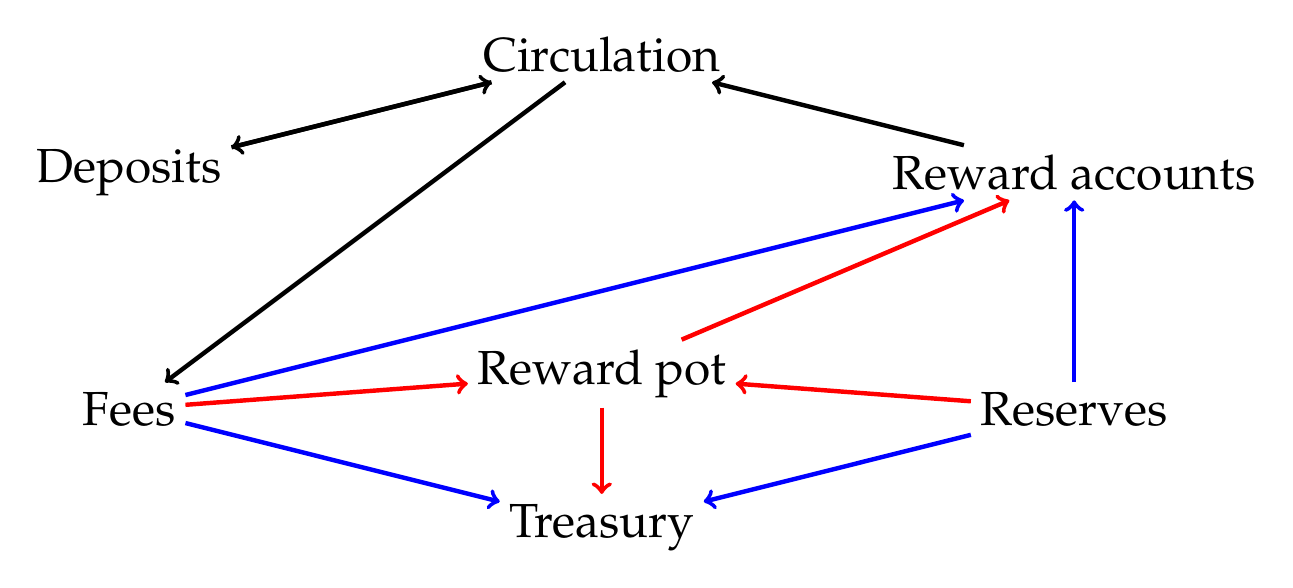
\begin{tikzpicture}
      [ x=30mm, y=30mm
      , direct/.style={black, draw}
      , implied/.style={blue, draw}
      , toTotPot/.style={red, draw}
      ]
    \node (C) at (3,2.5) {\LARGE Circulation};
    \node (R) at (5, 1) {\LARGE Reserves};
    \node (D) at (1, 2) {\LARGE Deposits};
    \node (FR) at (1,1) {\LARGE Fees};
    \node (RA) at (5, 2) {\LARGE Reward accounts};
    \node (T) at (3,0.5) {\LARGE Treasury};

    \draw[->, direct, ultra thick]
    (C) edge (D)
    (C) edge (FR)

    (D) edge (C)

    (RA) edge (C);

    \draw[->, implied, ultra thick]
    (FR) edge (T)
    (FR) edge (RA)

    (R) edge (T)
    (R) edge (RA);

    \node (TP) at (3, 1.15) {\LARGE Reward pot};

    \draw[->, toTotPot, ultra thick]
    (FR) edge (TP)
    (R) edge (TP)

    (TP) edge (RA)
    (TP) edge (T);
    \end{tikzpicture}
  \end{center}
  \caption{Preservation of Value}
  \label{fig:fund-preservation}
\end{figure}

Figure~\ref{fig:defs:reward-update} defines a reward update.
It consists of four pots:
\begin{itemize}
  \item The change to the treasury. This will be a positive value.
  \item The change to the reserves. This will be a negative value.
  \item The map of new individual rewards (to be added to the existing rewards).
  \item The change to the fee pot. This will be a negative value.
    rewards.
\end{itemize}

%%
%% Figure - Reward Update Defs
%%
\begin{figure}[htb]
  \emph{Reward Update}
  \begin{equation*}
    \RewardUpdate =
    \left(
      \begin{array}{r@{~\in~}ll}
        \Delta t & \Coin & \text{change to the treasury} \\
        \Delta r & \Coin & \text{change to the reserves} \\
        \var{rs} & \AddrRWD\mapsto\Coin & \text{new individual rewards} \\
        \Delta f & \Coin & \text{change to the fee pot} \\
      \end{array}
    \right)
  \end{equation*}
  %
  \caption{Rewards Update type}
  \label{fig:defs:reward-update}
\end{figure}

\clearpage

Figure~\ref{fig:functions:reward-update-creation} defines two functions,
$\fun{createRUpd}$ to create a reward update and $\fun{applyRUpd}$ to apply a
reward update to an instance of $\EpochState$.

The $\fun{createRUpd}$ function does the following:
\begin{itemize}
  \item Note that for all the calculations below, we use the previous protocol parameters
    $\var{prevPp}$, which corresponds to the parameters during the epoch for which we
    are creating rewards.
  \item First we calculate the change to the reserves,
    as determined by the $\rho$ protocol parameter.
  \item Next we calculate $\var{rewardPot}$, the total amount of coin available for rewards this
    epoch, as described in section 6.4 of \cite{delegation_design}. It consists of:
    \begin{itemize}
      \item The fee pot, containing the transaction fees from the epoch.
      \item The amount of monetary expansion from the reserves, calculated above.
    \end{itemize}
    Note that the fee pot is taken from the snapshot taken at the epoch boundary.
    (See~Figure\ref{fig:rules:snapshot}).
  \item Next we calculate the proportion of the reward pot that will move to the treasury,
    as determined by the $\tau$ protocol parameter. The remaining pot is called the
    $\var{R}$, just as in section 6.5 of \cite{delegation_design}.
  \item The rewards are calculated, using the oldest stake distribution snapshot (the one
    labeled ``go'').
    As given by $\fun{maxPool}$, each pool can receive a maximal amount, determined by its
    performance.  The difference between the maximal amount and the actual amount received is
    added to the amount moved to the treasury.
  \item The fee pot will be reduced by $\var{feeSS}$.
\end{itemize}

Note that fees are not explicitly removed from any account:
the fees come from transactions paying them and are accounted for whenever
transactions are processed.

The $\fun{applyRUpd}$ function does the following:
    \begin{itemize}
      \item Adjust the treasury, reserves and fee pots by the appropriate amounts.
      \item Add each individual reward to the global reward mapping.
        We must be careful, though, not to give out rewards to accounts
        that have been deregistered after the reward update was created.
        \begin{itemize}
          \item Rewards for accounts that are still registered are added to the reward mappings.
          \item The sum of the unregistered rewards are added to the reserves.
            % TODO - We may want to add these to the treasury instead, to be consistent with our other choices.
        \end{itemize}
    \end{itemize}

These two functions will be used in the blockchain transition systems in Section~\ref{sec:chain}.
In particular,
$\fun{createRUpd}$ will be used in Equation~\ref{eq:reward-update},
and $\fun{applyRUpd}$ will be used in Equation~\ref{eq:new-epoch}.

%%
%% Figure - The Reward Update Creation
%%
\begin{figure}[htb]
  \emph{Calculation to create a reward update}
  %
  \begin{align*}
    & \fun{createRUpd} \in \N \to \BlocksMade \to \EpochState \to \Coin \to \RewardUpdate \\
    & \createRUpd{slotsPerEpoch}{b}{es}{total} = \left(
      \Delta t_1,-~\Delta r_1+\Delta r_2,~\var{rs},~-\var{feeSS}\right) \\
    & ~~~\where \\
    & ~~~~~~~(\var{acnt},~\var{ss},~\var{ls},~\var{prevPp},~\wcard) = \var{es} \\
    & ~~~~~~~(\wcard,~\wcard,~\var{pstake_{go}},~\var{poolsSS},~\var{feeSS}) = \var{ss}\\
    & ~~~~~~~(\var{stake},~\var{delegs}) = \var{pstate_{go}} \\
    & ~~~~~~~(\wcard,~\var{reserves}) = \var{acnt} \\
    & ~~~~~~~\left(
      \wcard,~
      \left(
      \left(\var{rewards},~\wcard,~\wcard,~\wcard,~\wcard,~\wcard\right),~
      \wcard
      \right)
      \right) = \var{ls} \\
    & ~~~~~~~\Delta r_1 = \floor*{\min(1,\eta) \cdot (\fun{rho}~\var{prevPp}) \cdot
      \var{reserves}}
    \\
    & ~~~~~~~\eta =
      \begin{cases}
        1 & (\fun{d}~\var{prevPp})\geq 0.8 \\
        \frac{blocksMade}{\floor{(1-\fun{d}~\var{prevPp})\cdot\var{slotsPerEpoch} \cdot \ActiveSlotCoeff}}
          & \text{otherwise} \\
      \end{cases} \\
    & ~~~~~~~\var{rewardPot} = \var{feeSS} + \Delta r_1 \\
    & ~~~~~~~\Delta t_1 = \floor*{(\fun{tau}~\var{prevPp}) \cdot \var{rewardPot}} \\
    & ~~~~~~~\var{R} = \var{rewardPot} - \Delta t_1 \\
    & ~~~~~~~\var{circulation} = \var{total} - \var{reserves} \\
    & ~~~~~~~\var{rs}
      = \reward{prevPp}{b}{R}{(\dom{rewards})}{poolsSS}{stake}{delegs}{circulation} \\
    & ~~~~~~~\Delta r_{2} = R - \left(\sum\limits_{\_\mapsto c\in\var{rs}}c\right) \\
    & ~~~~~~~blocksMade = \sum_{\wcard \mapsto m \in b}m
  \end{align*}

  \caption{Reward Update Creation}
  \label{fig:functions:reward-update-creation}
\end{figure}

\begin{figure}[htb]
  \emph{Applying a reward update}
  %
  \begin{align*}
      & \fun{applyRUpd} \in \RewardUpdate \to \EpochState \to \EpochState \\
      & \fun{applyRUpd}~
      \left(
        \begin{array}{c}
          \Delta t \\
          \Delta r \\
          \var{rs} \\
          \Delta f \\
        \end{array}
    \right)
      \left(
        \begin{array}{c}
          \var{treasury} \\
          \var{reserves} \\
          ~ \\
          \var{rewards} \\
          \var{delegations} \\
          \var{ptrs} \\
          \var{genDelegs} \\
          \var{fGenDelegs} \\
          \var{i_{rwd}}
          \\~ \\
          \var{poolParams} \\
          \var{fPoolParams} \\
          \var{retiring} \\
          ~ \\
          \var{utxo} \\
          \var{deposited} \\
          \var{fees} \\
          \var{up} \\
          ~ \\
          \var{prevPp} \\
          \var{pp} \\
        \end{array}
      \right)
      =
      \left(
        \begin{array}{c}
          \varUpdate{\var{treasury} + \Delta t + \var{unregRU'}}\\
          \varUpdate{\var{reserves} + \Delta r}\\
          ~ \\
          \varUpdate{\var{rewards}\unionoverridePlus\var{regRU}} \\
          \var{delegations} \\
          \var{ptrs} \\
          \var{genDelegs} \\
          \var{fGenDelegs} \\
          \var{i_{rwd}}
          \\~ \\
          \var{poolParams} \\
          \var{fPoolParams} \\
          \var{retiring} \\
          ~ \\
          \var{utxo} \\
          \var{deposited} \\
          \varUpdate{\var{fees}+\Delta f} \\
          \var{up} \\
          ~ \\
          \var{prevPp} \\
          \var{pp} \\
        \end{array}
    \right) \\
    & ~~~\where \\
    & ~~~~~~~\var{regRU}=(\dom{rewards})\restrictdom rs\\
    & ~~~~~~~\var{unregRU}=(\dom{rewards})\subtractdom rs\\
    & ~~~~~~~\var{unregRU'}=\sum\limits_{\wcard\mapsto c\in\var{unregRU}} \var{c}\\
  \end{align*}

  \caption{Reward Update Application}
  \label{fig:functions:reward-update-application}
\end{figure}

\clearpage

\section{Blockchain layer}
\label{sec:chain}

\newcommand{\Proof}{\type{Proof}}
\newcommand{\Seedl}{\mathsf{Seed}_\ell}
\newcommand{\Seede}{\mathsf{Seed}_\eta}
\newcommand{\activeSlotCoeff}[1]{\fun{activeSlotCoeff}~ \var{#1}}
\newcommand{\slotToSeed}[1]{\fun{slotToSeed}~ \var{#1}}
\newcommand{\isOverlaySlot}[3]{\fun{isOverlaySlot}~\var{#1}~\var{#2}~\var{#3}}

\newcommand{\T}{\type{T}}
\newcommand{\vrf}[3]{\fun{vrf}_{#1} ~ #2 ~ #3}
\newcommand{\verifyVrf}[4]{\fun{verifyVrf}_{#1} ~ #2 ~ #3 ~#4}

\newcommand{\HashHeader}{\type{HashHeader}}
\newcommand{\HashBBody}{\type{HashBBody}}
\newcommand{\bhHash}[1]{\fun{bhHash}~ \var{#1}}
\newcommand{\bHeaderSize}[1]{\fun{bHeaderSize}~ \var{#1}}
\newcommand{\bSize}[1]{\fun{bSize}~ \var{#1}}
\newcommand{\bBodySize}[1]{\fun{bBodySize}~ \var{#1}}
\newcommand{\OCert}{\type{OCert}}
\newcommand{\BHeader}{\type{BHeader}}
\newcommand{\BHBody}{\type{BHBody}}

\newcommand{\bheader}[1]{\fun{bheader}~\var{#1}}
\newcommand{\hsig}[1]{\fun{hsig}~\var{#1}}
\newcommand{\bprev}[1]{\fun{bprev}~\var{#1}}
\newcommand{\bhash}[1]{\fun{bhash}~\var{#1}}
\newcommand{\bvkcold}[1]{\fun{bvkcold}~\var{#1}}
\newcommand{\bseedl}[1]{\fun{bseed}_{\ell}~\var{#1}}
\newcommand{\bprfn}[1]{\fun{bprf}_{n}~\var{#1}}
\newcommand{\bseedn}[1]{\fun{bseed}_{n}~\var{#1}}
\newcommand{\bprfl}[1]{\fun{bprf}_{\ell}~\var{#1}}
\newcommand{\bocert}[1]{\fun{bocert}~\var{#1}}
\newcommand{\bnonce}[1]{\fun{bnonce}~\var{#1}}
\newcommand{\bleader}[1]{\fun{bleader}~\var{#1}}
\newcommand{\hBbsize}[1]{\fun{hBbsize}~\var{#1}}
\newcommand{\bbodyhash}[1]{\fun{bbodyhash}~\var{#1}}
\newcommand{\overlaySchedule}[4]{\fun{overlaySchedule}~\var{#1}~\var{#2}~{#3}~\var{#4}}

\newcommand{\PrtclState}{\type{PrtclState}}
\newcommand{\PrtclEnv}{\type{PrtclEnv}}
\newcommand{\OverlayEnv}{\type{OverlayEnv}}
\newcommand{\VRFState}{\type{VRFState}}
\newcommand{\NewEpochEnv}{\type{NewEpochEnv}}
\newcommand{\NewEpochState}{\type{NewEpochState}}
\newcommand{\PoolDistr}{\type{PoolDistr}}
\newcommand{\BBodyEnv}{\type{BBodyEnv}}
\newcommand{\BBodyState}{\type{BBodyState}}
\newcommand{\RUpdEnv}{\type{RUpdEnv}}
\newcommand{\ChainEnv}{\type{ChainEnv}}
\newcommand{\ChainState}{\type{ChainState}}
\newcommand{\ChainSig}{\type{ChainSig}}



\subsection{Block Body Transition}
\label{sec:block-body-trans}


Figure~\ref{fig:rules:bbody} includes an additional check that the sum of the
execution units of all transactions in a block does not exceed the maximum total units per
block (specified in a protocol parameter).

\begin{figure}[ht]
  \begin{equation}\label{eq:bbody}
    \inference[Block-Body]
    {
      \var{txs} \leteq \bbody{block}
      &
      \var{bhb} \leteq \bhbody{(\bheader{block})}
      &
      \var{hk} \leteq \hashKey{(\bvkcold{bhb})}
      \\~\\
      \bBodySize{txs} = \hBbsize{bhb}
      &
      \fun{bbodyhash}~{txs} = \bhash{bhb}
      \\~\\
      \\
      \var{slot} \leteq \bslot{bhb}
      &
      \var{fSlot} \leteq \fun{firstSlot}~(\epoch{slot})
      \\~\\
      \hldiff{\sum_{tx\in txs} \fun{totExunits}~{tx} \leq \fun{maxBlockExUnits}~\var{pp}}
      \\~\\
      {
        {\begin{array}{c}
                 \bslot{bhb} \\
                 \var{pp} \\
                 \var{acnt}
        \end{array}}
        \vdash
             \var{ls} \\
        \trans{\hyperref[fig:rules:ledger-sequence]{ledgers}}{\var{txs}}
             \var{ls}' \\
      }
    }
    {
      {\begin{array}{c}
               \var{pp} \\
               \var{acnt}
      \end{array}}
      \vdash
      {\left(\begin{array}{c}
            \var{ls} \\
            \var{b} \\
      \end{array}\right)}
      \trans{bbody}{\var{block}}
      {\left(\begin{array}{c}
            \varUpdate{\var{ls}'} \\
            \varUpdate{\fun{incrBlocks}~{\left(\isOverlaySlot{fSlot}{(\fun{d}~pp)}{slot}\right)}~{hk}~{b}} \\
      \end{array}\right)}
    }
  \end{equation}
  \caption{BBody rules}
  \label{fig:rules:bbody}
\end{figure}

We have also defined a function that transforms the Shelley ledger state into
the corresponding Alonzo one, see Figure~\ref{fig:functions:to-shelley}. We
refer to the Shelley-era protocol parameter type as $\ShelleyPParams$, and the corresponding Alonzo
type as $\PParams$. We use the notation $\var{chainstate}_{x}$ to represent
variable $x$ in the chain state. We do not specify the variables that
remain unchanged during the transition.

%%
%% Figure - Shelley to Alonzo Transition
%%
\begin{figure}[htb]
  \emph{Types and Constants}
  %
  \begin{align*}
      & \NewParams = (\Language \mapsto \CostMod) \times \Prices \times \ExUnits \times \ExUnits \\
      & ~~~~~~~~ \times \N \times \Coin \times \N \times \N \\
      & \text{the type of new parameters to add for Alonzo}
      \nextdef
      & \var{ivPP} \in \NewParams \\
      & \text{the initial values for new Alonzo parameters}
  \end{align*}
  \emph{Shelley to Alonzo Transition Functions}
  %
  \begin{align*}
      & \fun{toAlonzo} : \ShelleyChainState \to \ChainState \\
      & \fun{toAlonzo}~\var{chainstate} =~\var{chainstate'} \\
      &~~\where \\
      &~~~~\var{chainstate'}_{pparams}~=~(\var{pp}\cup \var{ivPP})~ - ~\var{minUTxOValue}\\
      & \text{transform Shelley chain state to Alonzo state}
  \end{align*}
  \caption{Shelley to Alonzo State Transtition}
  \label{fig:functions:to-shelley}
\end{figure}

\include{software-updates}
\include{sts-overview}
\section{Formal Properties}
\label{sec:properties}

This appendix collects the main formal properties that the new ledger rules are expected to satisfy.
Note here that in every property in this section we consider a only phase-1 valid
transactions, ie. ones that can indeed get processed.

\begin{enumerate}[label=P{\arabic*}:\ ]
\item
  \emph{Consistency with Shelley.}
  \begin{itemize}
    \item properties 15.6 - 15.16 (except 15.8 and 15.13) hold specifically in the $\fun{txValTag}~tx~=~\True$ case, because
    the calculations refer to the UTxO as if it was updated by a scripts-validating transaction
    \item other properties hold as-is
  \end{itemize}

\item
  \emph{Consistency with Multi-Asset.}
  \begin{itemize}
    \item properties 8.1 and 8.2 hold specifically in the $\fun{txValTag}~tx~=~\True$ case, because
    the calculations refer to the UTxO as if it was updated by a scripts-validating transaction
    \item other properties hold as-is
  \end{itemize}
\end{enumerate}


\begin{definition}
  For a state $s$ that is used in any subtransaction of
  $\mathsf{CHAIN}$, we define $\Utxo(s) \in \UTxO$ to be the $\UTxO$
  contained in $s$, or an empty map if it does not exist. This is
  similar to the definition of $\Val$ in the Shelley specification.

  Similarly, we also define $\field_{v}~(s)$ for the field $v$ that is part of
  the ledger state $s$, referenced by the typical variable name (eg. $\var{fees}$
  for the fee pot on the ledger).
\end{definition}

We also define a helper function $\varphi$ as follows:
\[\varphi(x, tx) :=
  \begin{cases}
    x & \fun{txValTag}~tx = \True \\
    0 & \fun{txValTag}~tx = \False
  \end{cases}\]
This function is useful to distinguish between the two
cases where a transaction can mint tokens or not, depending on whether
its scripts validate.

\begin{property}[General Accounting]
  \label{prop:pov}
  The \emph{general accounting} property in Alonzo encompasses two parts
  \begin{itemize}
    \item preservation of value property expressed via the $\fun{produced}$ and $\fun{consumed}$
    calculations, applicable for transactions with $\fun{txValTag}~tx~=~\True$, which
    is specified as in the ShelleMA POV.
    \item the preservation of value for $\fun{txValTag}~tx~=~\False$, when
    only the collateral fees are collected into the fee pot.
  \end{itemize}

Both of these are expressed in the following lemma.

\begin{lemma}
  For all environments $e$, transactions $tx$ and states $s, s'$, if
  \begin{equation*}
    e\vdash s\trans{utxos}{tx}s'
  \end{equation*}
  then
  \begin{equation*}
    \Val(s) + \varphi(\fun{mint}~(\fun{txbody}~tx), tx) = \Val(s')
  \end{equation*}
\end{lemma}

\begin{proof}
  In the case that $\fun{txValTag}~tx = \True$ holds, the proof is
  identical to the proof of Lemma 9.1 of the multi-asset
  specification. Otherwise, the transition must have been done via the
  $\mathsf{Scripts-No}$ rule, which removes
  $\fun{collateral}~(\fun{txbody}~tx)$ from the UTxO, and increases the fee pot by the amount of the sum of Ada in the
  collateral UTxO entries. The value contained in $s$ is not changed.

  Note that in the $\fun{feesOK}$ function, there is a check that verifies
  that, in the case that there are phase-2 scripts, there are no non-Ada tokens in the UTxOs
  which the collateral inputs reference, so non-Ada tokens do not get minted, burned, or transfered
  in this case.
\end{proof}
\end{property}

\begin{property}[Extended UTxO Validation]
  \label{prop:fees-only}

  If a phase-1 valid transaction extends the UTxO, all its scripts validate
  (i.e. $\fun{txValTag}~tx = \True$).

  If a transaction is accepted and marked as paying collateral only
  (i.e. $\fun{txValTag}~tx = \False$), then the only change to the ledger
  when processing the transaction is that the collateral inputs
  are moved to the fee pot. In particular, it does not extend the UTxO.

  \begin{lemma}
    For all environments $e$, transactions $tx$ and states $s, s'$, if  and
    \begin{equation*}
      e\vdash s\trans{ledger}{tx}s'
    \end{equation*}
    then
    \[\Utxo(s') \nsubseteq \Utxo(s)~\Rightarrow~\fun{txValTag}~tx = \True \]

    Also,
    \[\fun{txvaltag}~tx = \False~ \Rightarrow~\]
    \begin{itemize}
      \item $ \field_{v}~(s') = \field_{v}~(s) \text{ for all } v~\neq~{fees}, ~v~\neq~{utxo}$
      \item $\field_{fees}~(s') = \field~\var{fees}~(s) + \fun{coin}~(\Val~(\fun{collateral}~{tx} \subtractdom \Utxo(s)))$
      \item $\Utxo(s') = \fun{collateral}~{tx} \subtractdom \Utxo(s)$
    \end{itemize}
  \end{lemma}

  \begin{proof}
    A ledger UTxO update is specified explicitly only by the $\mathsf{UTXOS}$ transition,
    and propagated (ie. applied as-specified) to a chain-state update via the
    $\mathsf{UTXO}$ and $\mathsf{UTXOW}$ transitions.

    The only case in which the $\mathsf{UTXOS}$ transition adds entries to the UTxO
    map is in the $\mathsf{Scripts-No}$ rule, when $\fun{txValTag}~tx = \True$.
    Adding entries to the UTxO map implies exactly that the updated map is not a
    submap of the original, so we get that

    \[\Utxo(s') \nsubseteq \Utxo(s)~\Rightarrow~\fun{txValTag}~tx = \True \]

   In the case that $\fun{txValTag}~tx = \False$, $\mathsf{LEDGER}$ calls the rule
   that does not update $\DPState$ at all, only the $\UTxOState$. This state update is specified
   in the $\mathsf{UTXOS}$ transition (and applied via the $\mathsf{UTXO}$ and $\mathsf{UTXOW}$ transitions).

   The only parts of the state that are updated are
   \begin{itemize}
     \item the fee pot, which is increased by the amount of the sum of Ada in the
     collateral UTxO entries, and
     \item the UTxO, where the collateral entries
     are removed.
   \end{itemize}
  \end{proof}
\end {property}

\begin{property}[Validating when No NN Scripts]
  \label{prop:is-valid}

Whenever a valid transaction does not have any phase-2 scripts, its
$\fun{txValTag} = \True$.

\begin{lemma}
  For all environments $e$, transactions $tx$ and states $s, s'$ such that
  \begin{equation*}
    e\vdash s\trans{ledger}{tx}s',
  \end{equation*}
  If $\range (\fun{txscripts}~tx) \cap \ScriptPhTwo = \emptyset$
  then $\fun{txValTag} = \True$.
\end{lemma}
\begin{proof}
  With the same argument as previously, we only need to discuss the
  equivalent claim for the $\mathsf{UTXOS}$ transition. Under these
  assumptions, $\var{sLst} := \fun{collectTwoPhaseScriptInputs}$ is an empty
  list. Thus $\fun{evalScripts}~sLst = \True$, and the transition rule
  had to be $\mathsf{Scripts{-}Yes}$.
\end{proof}
\end{property}

\begin{property}[Paying fees]
  \label{prop:pay-fees}

In the case that all phase-2 scripts in a transaction validate, the transaction pays
at least the minimum transaction fee amount into the fee pot. In the case that
some do not validate, it must pay at least the percentage of the minimum fee
the collateral is required to cover.

\begin{lemma}
  For all environments $e$, transactions $tx$ and states $s, s'$ such that
  \begin{equation*}
    e\vdash s\trans{ledger}{tx}s'
  \end{equation*}
  The following holds : \\
  $\field_{fees}~(s')~\geq~\field_{fees}~(s)~+
  \begin{cases}
    \fun{minfee}~{tx} & \fun{txValTag} = \True \\
    \fun{quot}~(\fun{collateralPercent}~(\field_{pp}~(s)))~*~(\fun{minfee}~{tx})~100 & \fun{txValTag} = \False\\
  \end{cases}$.
\end{lemma}
\begin{proof}
  The fee pot is updated by the $\mathsf{Scripts{-}Yes}$ and the $\mathsf{Scripts{-}No}$
  rules, one of which is necessarily called by a valid transaction via the sequence
  of transitions called in the order $\mathsf{LEDGER}, \mathsf{UTXOW}, \mathsf{UTXO}, \mathsf{UTXOS}$.

  The $\mathsf{Scripts{-}Yes}$ rule (i.e. $\fun{txValTag} = \True$)
  transfers the amount of lovelace in the $\fun{txfee}$ field of the
  transaction to the fee pot, which is checked to be at least the $\fun{minfee}$
  by $\fun{feesOK}$ in the $\mathsf{UTXO}$ transition. So, we get

  \[\field_{fees}~(s')~=~\field_{fees}~(s)~+~\fun{txfee}~{tx}~\geq~\field_{fees}~(s)~+~\fun{minfee}~{tx}\]

  The $\mathsf{Scripts{-}No}$ rule (i.e. $\fun{txValTag} = \False$) removes the
  $\fun{collateral}$ inputs from the
  UTxO, and adds the the balance of these realized inputs to the fee pot.

  \[\field_{fees}~(s')~=~field_{fees}~(s)~+~\fun{ubalance}~(\fun{collateral}~{txb} \restrictdom \var{utxo})\]

  We can conclude that $\fun{txrdmrs}$ is non-empty whenever $\fun{txValTag} = \False$
  from the following observations :
  \begin{itemize}
    \item $\fun{txValTag} = \False$ whenever $\fun{evalScripts}$ fails.
    \item $\fun{evalScripts}$ is a $\wedge$-fold over a list of scripts and
    their inputs, containing all scripts that need to be run to validate this transaction
    \item All phase-1 scripts must succeed, as this is checked in phase-1 validation (UTXOW
    rule check). Therefore,
    $\fun{evalScripts}$ encounters a failing script which is phase-2.
    \item All phase-2 scripts necessarily have an associated redeemer attached to the
    transaction (UTXOW rule check)
  \end{itemize}

  See Property~\ref{prop:fixed-inputs} for more details on what inputs $\fun{evalScripts}$ has,
  and what we can say about the outcome of its computation with respect to its inputs.

  The $\fun{feesOK}$ check enforces that if a transaction has a non-empty
  $\fun{txrdmrs}$ field, the balance of the realized collateral inputs
  (which $\field_{fees}~(s)$ is increased by as part of processing $tx$) is

  \[\fun{ubalance}~(\fun{collateral}~{txb} \restrictdom \var{utxo})~\geq~\fun{quot}~(\txfee~{txb} * (\fun{collateralPercent}~pp))~100\]

  which, since $\txfee~{txb}~\geq~\fun{minfee}~{txb}$, gives

  \[ \geq~\fun{quot}~(\fun{minfee}~{txb} * (\fun{collateralPercent}~pp))~100)) \]

  where $\fun{txbody}~{tx}~=~{txb}$. This shows that the total collateral that gets
  moved into the fee pot from the UTxO by the $\mathsf{Scripts{-}No}$ rule is at
  least the minimum transaction fee scaled by the collateral percent parameter.

  \[\field_{fees}~(s')~\geq~\field_{fees}~(s)~+~\fun{quot}~(\fun{minfee}~{txb} * (\fun{collateralPercent}~pp))~100))\]
\end{proof}

An immediate corollary to this property is that when the $\fun{collateralPercent}$ is set to 100 or more,
the transaction always pays at least the minimum fee. This, in turn, implies that it
pays at least the fee that it has stated in the $\fun{txfee}$ field.

\begin{corollary}
  For all environments $e$, transactions $tx$ and states $s, s'$ such that
  \begin{equation*}
    e\vdash s\trans{ledger}{tx}s'~~\wedge~~\fun{collateralPercent}~(\field_{pp}~(s)) \geq 100
  \end{equation*}
  The following holds :
  \[\field_{fees}~(s')~\geq~\field_{fees}~(s)~+~\fun{minfee}~{tx} \]
\end{corollary}

\begin{proof}
  In both two cases in the lemma above, the $\field_{fees}$ field in the ledger state
  is increased by at least $\fun{minfee}~{tx}$ :
  \begin{itemize}
    \item when $\fun{txValTag} = \True$, the lemma states already that
    \[\field_{fees}~(s')~\geq~\field_{fees}~(s)~+~\fun{minfee}~{tx}\]
    \item when $\fun{txValTag} = \False$, we have
    $ \field_{fees}~(s')~\geq~\field_{fees}~(s)~+~\fun{quot}~(\fun{minfee}~{txb} * (\fun{collateralPercent}~pp))~100$ \\
    $~~~\geq~\field_{fees}~(s)~+~\fun{quot}~(\fun{minfee}~{tx}~*~100)~100$ \\
    $~~~=~\field_{fees}~(s)~+~\fun{minfee}~{tx}$
  \end{itemize}
\end{proof}

\end{property}

\begin{property}[Correct tag]
  \label{prop:correct-tag}

The $\fun{txValTag}~tx$ tag of a phase-1 valid transaction must match the result of the $\fun{evalScripts}$
function for that transaction.

\begin{lemma}
  For all environments $e$, transactions $tx$ and states $s, s'$ such that
  \begin{equation*}
    e\vdash s\trans{utxos}{tx}s',
  \end{equation*}
  The following holds :
    \[\fun{txValTag}~tx ~=~ \fun{evalScripts}~{tx}~{sLst} \]
  where
  \[ \var{sLst} \leteq \fun{collectTwoPhaseScriptInputs} ~\field_{pp}(s)~\var{tx}~ \Utxo(s) \]
\end{lemma}
\begin{proof}
  Inspecting the $\mathsf{Scripts{-}Yes}$ and the $\mathsf{Scripts{-}No}$ rules of the $\mathsf{UTXOS}$ transition,
  we see that both the $\fun{txValTag}$ and the result of $\fun{evalScripts}$
  are $\True$ in the former, and $\False$ in the latter.
\end{proof}
\end{property}

\begin{property}[Replay protection]
  \label{prop:replay}

A transaction always removes at least one UTxO entry from the ledger, which provides
replay protection.

\begin{lemma}
  For all environments $e$, transactions $tx$ and states $s, s'$ such that
  \begin{equation*}
    e\vdash s\trans{ledger}{tx}s',
  \end{equation*}
  The following holds : $\Utxo~(s)~\nsubseteq~\Utxo~(s')$.
\end{lemma}
\begin{proof}
  The UTxO is updated by the $\mathsf{Scripts{-}Yes}$ and the $\mathsf{Scripts{-}No}$
  rules, on of which is necessarily called by a valid transaction. Both of these
  rules remove UTxOs corresponding to a set of inputs.

  In both cases, there is a check that the removed inputs set is non-empty.
  The $\mathsf{Scripts{-}Yes}$ rule of the $\mathsf{UTXOS}$ transition
  removes the UTxOs associated with the input set $\fun{txinputs}~{tx}$ from the ledger.
  The $\fun{txinputs}~{tx}$ set must be non-empty because there is a check in the
  $\mathsf{UTXO}$ rule (which calls $\mathsf{UTXOS}$) that ensure this is true.

  For the $\mathsf{Scripts{-}No}$ rule of the $\mathsf{UTXOS}$ transition
  removes the UTxOs associated with the input set $\fun{collateral}~{tx}$ from the ledger.
  The $\fun{collateral}~{tx}$ set must be non-empty because
  the $\fun{feesOK}$ function (called by the same rule that calls $\mathsf{UTXO},
  \mathsf{UTXOS}$) ensures that in the case that the $tx$ contains phase-2 scripts,
  $\fun{collateral}~{tx}$ must be non-empty.

  Note that by property~\ref{prop:is-valid}, phase-2 scripts must always be present
  if $\fun{txValTag}~tx = \False$ (that is, whenever $\mathsf{Scripts{-}No}$ rule is used).
\end{proof}
\end{property}

\begin{property}[UTxO-changing transitions]
  \label{prop:utxo-change}

The $\mathsf{UTXOS}$ transition fully specifies the change in the ledger $\UTxO$
for each transaction.

\begin{lemma}
  For all environments $e$, transitions $\mathsf{TRNS}$, transactions $tx$ and states $s, s'$ such that
  \begin{equation*}
    e\vdash s\trans{trns}{tx}s'
  \end{equation*}
  The following holds :
  \begin{equation*}
    \Utxo(s) \neq \Utxo(s')~\Rightarrow~e'\vdash u\trans{utxos}{tx}u'
  \end{equation*}
  where $\Utxo(s) = \Utxo(u)~\wedge~\Utxo(s') = \Utxo(u')$ for some environment $e'$,
  and states $u, u'$.
\end{lemma}
\begin{proof}
  By inspecting each transition in this specification, as well as those inherited from the
    Shelley one, we see that a non-trivial update from the UTxO of $s$ to that of $s'$
    must be done by $\mathsf{UTXOS}$. Every other transition that changes the UTxO and
    has a signal of type $\Tx$ only applies the $\mathsf{UTXOS}$.
\end{proof}
\end{property}

\begin{property}[Script interpreter arguments are fixed (deterministic script evaluation)]
  \label{prop:fixed-inputs}

For this property, we make some assumptions about things that are outside the scope of this specifications :

\begin{itemize}
  \item The Plutus script
  interpreter is a pure function that receives only the arguments provided by the ledger when it is
  invoked by calling the $\fun{runPLCScript}$ function. We assume that this is
  also true in an implementation. In particular, the interpreter does not
  obtain any system randomness, etc.

  \item We assume that constructing the validation context from $\TxInfo$ and
  the $\ScriptPurpose$ by $\fun{valContext}$ is deterministic.

  \item We do not need to check here that the hashes that are the keys of the
  $\fun{txscripts}$ and $\fun{txdats}$ fields match the computed hashes of the scripts and
  datum objects they index. This is because these hashes must be computed as part of
  the deserialization of a transaction (see the CDDL specification),
  instead of being transmitted as part of the transaction and then checked. We
  assume these hashes are correct.

  \item We assume that the consensus
  function $\fun{epochInfoSlotToUTCTime}$ for converting a slot interval into a
  system time interval is deterministic.

  \item We assume that the two global
  constants, $\EpochInfo$ and $\SystemStart$, which it also takes as parameters,
  cannot change within the span of any interval for which $\fun{epochInfoSlotToUTCTime}$
  is able to convert both endpoints to system time.
\end{itemize}

The assumptions above are implicit in the functional style of definitions in this
specification, but they are worth pointing out for implementation.
With these assumptions in mind, we can say that
script evaluation is deterministic.

We split this result into a lemma and its corollary :

\begin{itemize}
  \item First, we demonstrate that all the scripts and their arguments that are
  collected for phase-2 validation are the same for two phase-1 valid transactions with the same body,
  independent of the (necessarily valid) ledger state to which they are being applied

  \item Second, we derive the corollary that under the same validity assumptions,
  phase-2 validation results in the same outcome for both transactions
\end{itemize}

\begin{lemma}
  \label{lem:inputs}
  For all environments $e, e'$, transactions $tx, tx'$ and states $s, s', u, u'$ such that
  $e$ and $s$ are subsets of fields of some valid chain state $c$, and
  $e'$ and $s'$ are subsets of fields of some valid chain state $c'$,

  \begin{equation*}
    e\vdash s\trans{ledger}{tx}s', \\
    e'\vdash u\trans{ledger}{tx'}u', \\
    \txbody{tx} = \txbody{tx'}
  \end{equation*}

  The following holds :

  \[\fun{toSet}~(\fun{collectTwoPhaseScriptInputs} ~\field_{pp}(s)~\var{tx}~ \Utxo(s))\]
  \[ = \]
  \[\fun{toSet}~(\fun{collectTwoPhaseScriptInputs} ~\field_{pp}(u)~\var{tx'}~ \Utxo(u))\]

\end{lemma}
\begin{proof}

    The $\fun{collectTwoPhaseScriptInputs}$
    function (see \ref{fig:functions:script2})
    constructs a list where each entry contains a Plutus script
    and the argumets passed to the interpreter for its evaluation.

    To show that $\fun{collectTwoPhaseScriptInputs}$ returns a list containing
    the same elements for both $tx$ and $tx'$, we observe that
    the set of elements from which this list is produced via $\fun{toList}$
    is generated using the following functions, as well as set comprehension
    and list operations.
    We demonstrate that the functions used in this definition
    produce the same output for $tx$ and $tx'$, as all the data they
    inspect is fixed by the transaction body :

    \begin{itemize}
      \item $\fun{scriptsNeeded}$ : The $\PolicyID$, $\AddrRWD$, and $\DCert$ data
      output by this function as the second term of the hash-purpose pair
      is obtained directly from the $\fun{mint}$, $\fun{txwdrls}$,
      $\fun{txcerts}$ fields of the transaction, which are all fixed by the
      body of the transaction. These types of script purposes all include
      the hash of the validating script.

      The only other data this function inspects is the UTxO entries associated
      with the $\fun{txinputs}$ (passed via the $\UTxO$ argument) to get the realized inputs.
      We know that the UTxO is a field in a valid chain state for both the phase-1 valid
      transactions $tx$ and
      the $tx'$ ($\Utxo(s)$ and $\Utxo(u)$, respectively). This means that the $\TxId$
      in each input present in either UTxO is a hash of the body of the transaction
      containing the $\TxOut$ part of the UTxO entry indexed by that input. The
      order of the outputs is also fixed by the body, which fixes the $\Ix$ of
      the entry.

      A different value in output part of the UTxO entry (or a different order of
      outputs) would necessarily imply
      that the hash of the body containing that output must be different.
      Therefore, for all Plutus script-locked realized inputs of either transaction,
      the script hash in the payment credential of the address
      (and, by the same argument, the datum hash) are fixed by the inputs in body of the
      transaction, despite not being explicitly contained in it. We then get that

      \[ \fun{scriptsNeeded}~\Utxo(s)~tx = \fun{scriptsNeeded}~\Utxo(u)~tx' \]

      \item $\fun{getDatum}$ : In the case the script purpose
      is of the input type, the datum this function returns is one that
      is associated with the corresponding realized input. More precisely, it is the datum whose
      hash is specified in the realized input, and is looked up by hash in the $\fun{txdats}$
      transaction field. If there is no datum hash in the realized input, or the script purpose
      is of a non-input type, the empty list is returned.

      The $\mathsf{UTXOW}$ rule checks that the transaction is carrying all datums corresponding
      to its realized inputs. Since the inputs (and realized inputs) are the same
      for $tx$ and $tx'$ (fixed by the body), this guarantees that
      of the datum hashes in the realized inputs (and therefore, their preimages)
      are the same as well.

      \item $\fun{txscripts}$ : in the $\mathsf{UTXOW}$ rule, there is a check that all the
      script preimages of the script hashes returned by the $\fun{scriptsNeeded}$
      function must be present in this field.

      \item $\fun{indexedRdmrs}$ : like $\fun{scriptsNeeded}$, this function
      examines four fields fixed by the transaction body ($\fun{mint}$, $\fun{txwdrls}$,
      $\fun{txcerts}$, and $\fun{txinputs}$).
      It also looks at data in the $\fun{txrdmrs}$ field, which is fixed
      by the transaction body via the $\fun{scriptIntegrityHash}$
      hash. This is done as follows: the $\mathsf{UTXOW}$ rule verifies that this
      hash-containing field matches the computed hash
      of the preimage constructed from several fields of the transaction,
      including $\fun{txrdmrs}$ (this calculation
      is done by the $\fun{hashWitnessPPData}$ function).

      \item $\fun{language}$ : this is directly conveyed by the type of a script.

      \item $\fun{costmdls}$ : The hash calculated by the $\fun{hashWitnessPPData}$
      function and compared to the hash value in the $\fun{scriptIntegrityHash}$ field
      must include in the preimage the current cost models of
      all script languages of scripts carried by the transaction. Recall that
      if a cost model changed between when a transaction was submitted and the
      time at which it was processed, the field and the calculated hash values
      will not match.

      \item $\fun{valContext}$ and $\fun{txInfo}$ :
      The $\fun{valContext}$ function is assumed deterministic.
      All fields of the $\TxInfo$
      structure, with the exceptions listed below,
      are straightforward translations of the corresponding transaction body fields (see \ref{sec:txinfo}) that
      are given no additional arguments,
      and therefore completely determined by $tx$ and $tx'$. The fields not directly
      appearing in the body are :

      \begin{itemize}
        \item $\fun{txInfoInputs}$ : this field contains the realized inputs of
        the transaction which are fixed by the transaction and the unique
        UTxO entries to which the inputs correspond. As explained above,
        accessing information in realized inputs for script evaluation
        does not break determinism.

        \item $\fun{txInfoValidRange}$ : this field contains the transaction
        validity interval as system time (converted from the slot numbers, which are
        used to speficy the interval in the transaction body). This conversion is
        done by a function defined in the consensus layer, and takes two global
        constants in addition to the slot interval itself. Since the slot interval
        conversion function $\fun{epochInfoSlotToUTCTime}$ necessarily
        succeeds if both $tx$ and $tx'$ pass phase-1 validation, the additional
        global constant arguments must be the same (by assumption). The determinism of this conversion
        is one of the assumptions of this property, and thus gives the same ouput
        for both transactions.

        \item $\fun{txInfoData}$ : this field is populated with the datums (and their
        hashes) in the transaction field $\fun{txdats}$, which are fixed by the body
        via the $\fun{scriptIntegrityHash}$ field.

        \item $\fun{txInfoId}$ : this field contains the hash of the transaction body,
        which is clearly the same for transactions with the same body.
      \end{itemize}

      Therefore, each field of the $\TxInfo$ structure is
      the same for two transactions with the same body, ie.

      \[ \fun{txInfo}~\PlutusVI~\Utxo(s)~\var{tx} = \fun{txInfo}~\PlutusVI~\Utxo(u)~\var{tx'}\]

    \end{itemize}
\end{proof}

We can now make the general statement about evaluation of all scripts done in
phase-2 validation : for any phase-1 valid transactions with the same body,
the outcome of phase-2 script evaluation is the same. We make the same assumptions
as in Lemma \ref{lem:inputs}.

\begin{corollary}
  For all environments $e, e'$, transactions $tx, tx'$ and states $s, s', u, u'$ such that
  \begin{equation*}
    e\vdash s\trans{ledger}{tx}s', \\
    e'\vdash u\trans{ledger}{tx'}u', \\
    \txbody{tx} = \txbody{tx'}
  \end{equation*}
  The following holds :

  \[\fun{evalScripts}~{tx}~ (\fun{collectTwoPhaseScriptInputs} ~\field_{pp}(s)~\var{tx}~ \Utxo(s))\]
  \[ = \]
  \[\fun{evalScripts}~{tx'}~ (\fun{collectTwoPhaseScriptInputs} ~\field_{pp}(u)~\var{tx'}~ \Utxo(u))\]

\end{corollary}

\begin{proof}
  Let us consider the use of arguments of $\fun{evalScripts}$ (see Figure \ref{fig:functions:script2}).
  The first argument (of type $\Tx$) is only inspected in the case that the script $sc$ (the first element
    in the pair at the head of the list of script-arguments pairs is a phase-1 script. Since all phase-1 scripts
    are checked in phase one of validation (see \ref{fig:rules:utxow-alonzo}) by calling $\fun{validateScript}$
    on all scripts attached to the transaction. For this to apply to $sc$, we must also show
    that $sc$ is a script attached to the transaction (see the second argument explanation).
    Note also that the $tx$ argument passed to $\fun{evalScripts}$ at the use site (in the $\mathsf{UTXOS}$ transition)
    is the same, unmodified $tx$ as is the signal for the LEDGER transition. We verify this by inspecting
    the sequence of transitions through which it is propagated
    ($\mathsf{UTXOS}$, $\mathsf{UTXO}$, $\mathsf{UTXOW}$, and $\mathsf{LEDGER}$), and their signals.

    This allows us to conclude that at every step of the iteration over the script-arguments pairs list,
    the first argument to $\fun{evalScripts}$,

    \begin{itemize}
      \item has no impact on the outcome of script evaluation in the case the script
      being validated at this step is phase-2, as it is competely ignored, and,

      \item because $\fun{collectTwoPhaseScriptInputs}$ filters out all phase-1 scripts,
      is, in fact, ignored always.
    \end{itemize}

    The second argument to $\fun{evalScripts}$, ie. the list of scripts and their arguemnts,
    has already been shown to contain the same tuples for both transactions in the lemma above.
    The order of the list does not affect the validation outcome, since the interpreter is run
    on each tuple of a script and its arguments independently of all other tuples in the list.
    The function $\fun{evalScripts}$ is a $\wedge$-fold over the list. Thus, we may ignore the order
    of the elements in the generated list as it does not affect the evaluation outcome.

    From this we may conclude that the outcome of both phase-1 and phase-2 script evaluations
    at each step of $\fun{evalScripts}$ must be the same for $tx$ and $tx'$. Therefore,
    the $\wedge$-fold of them done by $\fun{evalScripts}$ also produces the same outcome
    for both transactions.

\end{proof}
\end{property}

\begin{property}[Zipper property]
  \label{prop:zipper}

We say that a transaction is in \emph{zipped} form when it does not have
separate fields for scripts, datum objects, and redeemers. Instead, these are
all placed directly alongside the parts which they are meant to validate.
For example, the $\fun{mint}$ field would contain the full script instead of
just the policy ID script hash.

A valid transaction can be expressed in zipped form, which
is isomorphic to the original transaction. Let us define the zipped representation
of a transaction --- see Figure \ref{fig:zipped-types}.

\begin{figure*}[htb]
  \emph{Zipped Transaction Types}
  %
  \begin{equation*}
    \begin{array}{r@{~~}l@{~~}l@{\qquad}l}
      \TxIn_{zip} ~=~&
       (\TxIn \times \TxOut)  ~\uniondistinct \\
       & (\TxIn \times \TxOut \times \Script \times \Data^? \times \Data^? \times \CostMod^? \times \ExUnits^?)\\
      \Value_{zip} ~=~&
      (\Coin \times ((\PolicyID \times \Script \times \Data^? \times \CostMod^? \times \ExUnits^?) \\
      & \mapsto_0 (\AssetName \mapsto_0 \Quantity))) \\
      \Wdrl_{zip} ~=~& ((\AddrRWD \times \VKey \times \Sig) \mapsto \Coin) ~ \uniondistinct \\
      & ((\AddrRWD \times \Script \times \Data^? \times \CostMod^? \times \ExUnits^?) \mapsto \Coin) \\
      \TxOut_{zip}~=~& \TxOut \times \Data^? \\
      \DCert_{zip}~=~& (\DCert \times \VKey \times \Sig) ~ \uniondistinct \\
      & (\DCert \times \Script \times \Data^? \times \CostMod^? \times \ExUnits^?)
    \end{array}
  \end{equation*}
  %
  \emph{Transaction Types}
  %
  \begin{equation*}
    \begin{array}{r@{~~}l@{~~}l@{\qquad}l}
      \var{txbody} ~\in~ \TxBody_{zip}~=~
      & \hldiff{\powerset{\TxIn_{zip}}} & \fun{txinputs}& \text{Inputs}\\
      & \times ~\hldiff{\powerset{\TxIn}_{zip}} & \fun{collateral} & \text{Collateral inputs}\\
      & \times ~(\Ix \mapsto \hldiff{\TxOut_{zip}}) & \fun{txouts}& \text{Outputs}\\
      & \times~ \hldiff{\seqof{\DCert_{zip}}} & \fun{txcerts}& \text{Certificates}\\
       & \times ~\hldiff{\Value_{zip}}  & \fun{mint} &\text{A minted value}\\
       & \times ~\Coin & \fun{txfee} &\text{Total fee}\\
       & \times ~\ValidityInterval & \fun{txvldt} & \text{Validity interval}\\
       & \times~ \hldiff{\Wdrl_{zip}}  & \fun{txwdrls} &\text{Reward withdrawals}\\
       & \times ~\Update^?  & \fun{txUpdates} & \text{Update proposals}\\
       & \times ~\powerset{\KeyHash} & \fun{reqSignerHashes} & \text{Hashes of VKeys passed to scripts}\\
       & \times ~\Network^? & \fun{txnetworkid} & \text{Tx network ID}\\
    \end{array}
  \end{equation*}
  %
  \begin{equation*}
    \begin{array}{r@{~~}l@{~~}l@{\qquad}l}
      \var{tx} ~\in~ \Tx_{zip} ~=~
      & \TxBody_{zip} & \fun{txbody} & \text{Body}\\
      & (\VKey \mapsto \Sig) & \fun{txwitsVKey} & \text{VKey signatures}\\
      & \times ~\AuxiliaryData^? & \fun{auxiliaryData}&\text{Auxiliary data}\\
      & \times ~\IsValid & \fun{isValid} & \text{Validation tag}\\
    \end{array}
  \end{equation*}
  \caption{Zipped transaction types}
  \label{fig:zipped-types}
\end{figure*}

\begin{lemma}
  For all environments $e$, phase-1 valid transactions $tx$ and states $s, s'$ such that
  \begin{equation*}
    e\vdash s\trans{utxow}{tx}s',
  \end{equation*}
  The zipping and unzipping functions compose as in Figure \ref{fig:zip}.

\begin{figure*}[htb]
  \emph{Zipping and Unzipping Functions}
  %
  \begin{align*}
    & \fun{zip}~\in~(\Tx \times \UTxO \times \PParams)~ \to~ (\Tx_{zip} \times \UTxO \times \PParams) \\
    & \fun{zip}~(\var{tx},~\var{utxo},~\var{pp})=~(\fun{ziptx}~({tx},~{utxo},~{pp}),~\var{utxo},~\var{pp}) \\
    & \where \\
    &~~~~\fun{field}~(\fun{ziptx}~({tx},~{utxo},~{pp}))~=~\\
    &~~~~~~~  \begin{cases}
        \fun{field}~\var{tx} & \fun{field} \notin \{\fun{txinputs},~\fun{collateral},~\fun{txouts},~\fun{txcerts},~\fun{mint},~\fun{txwdrls},\\
        & \fun{scriptIntegrityHash}\} \\
        \fun{txinputs}_{zip}~{tx}~({txins},~{utxo},~{pp}) & \fun{field}~\in~\{~\fun{txinputs},~\fun{collateral} ~\}\\
        \fun{field}_{zip}~{tx}~(\fun{field}~{tx}) & \text{otherwise} \\
      \end{cases}
    \nextdef
    &\fun{txinputs}_{zip}~ \in~ \Tx \to (\powerset{\TxIn} \times \UTxO \times \PParams) \to \powerset{\TxIn_{zip}} \\
    &\fun{txinputs}_{zip}~{tx}~({txins},~{utxo},~{pp}) ~=~ \{ (txin,~txout,~\fun{paymentHK}~a,~sg)~\vert~\\
    & ~~~~{txin}\mapsto {(a, v, \wcard)}\in utxo,~(\fun{paymentHK}~a)\mapsto sg~\in~\fun{txwitsVKey}~tx \} \\
    & ~~~~\uniondistinct~ \{ (txin,~txout,~s,~d,~r,~exu,~cm)~\vert~\\
    & ~~~~{txin}\mapsto {(a, v, dh)}\in utxo,~(\fun{validatorHash}~a)\mapsto s~\in~\fun{txscripts}~tx, \\
    & ~~~~(s~\in~\ScriptPhTwo~\Rightarrow~(dh\mapsto d~\in~\fun{txdats}~tx,~(r, exu)~=~\fun{indexedRdmrs}~tx~txin), \\
    & ~~~~cm = (\fun{costmdls}~pp)~(\fun{language}~s)), \\
    & ~~~~(s~\notin~\ScriptPhTwo~\Rightarrow~(d=\Nothing,~r=\Nothing,~exu=\Nothing,~cm=\Nothing)\} \\
    \nextdef
    &\fun{collateral}_{zip}~ \in~ \Tx \to \powerset{\TxIn} \to \powerset{\TxIn_{zip}}\\
    &\fun{collateral}_{zip} ~=~ \fun{txinputs}_{zip}
    \nextdef
    &\fun{txouts}_{zip}~ \in~ \Tx \to (\Ix \mapsto \TxOut) \to (\Ix \mapsto \TxOut_{zip}) \\
    &\fun{txouts}_{zip}~{tx}~{txouts} ~=~
    \nextdef
    &\fun{txcerts}_{zip}~ \in~ \Tx \to \seqof{\DCert} \to \seqof{\DCert_{zip}} \\
    &\fun{txcerts}_{zip}~{tx}~{crts} ~=~
    \nextdef
    &\fun{mint}_{zip}~ \in~ \Tx \to \Value \to \Value_{zip} \\
    &\fun{mint}_{zip}~{tx}~{v} ~=~
    \nextdef
    &\fun{txwdrls}_{zip}~ \in~ \Tx \to \Wdrl \to \Wdrl_{zip} \\
    &\fun{txwdrls}_{zip}~{tx}~{wdrls} ~=~
    \nextdef
    &\fun{unzip}~\in~(\Tx_{zip} \times \UTxO \times \PParams)~ \to~ (\Tx \times \UTxO \times \PParams)
  \end{align*}
  %
  \emph{Zipping and Unzipping Function Composition}
  %
  \begin{align*}
    \fun{unzip}~(\fun{zip}~({tx},~{utxo},~{pp}))=~({tx},~{utxo},~{pp})
  \end{align*}
  \caption{Zipping and Unzipping Functions and Composition}
  \label{fig:zip}
\end{figure*}



\end{lemma}
\begin{proof}
  With the same argument as previously, we only need to discuss the
  equivalent claim for the $\mathsf{UTXOS}$ transition. Under these
  assumptions, $\var{sLst} := \fun{collectTwoPhaseScriptInputs}$ is an empty
  list. Thus $\fun{evalScripts}~sLst = \True$, and the transition rule
  had to be $\mathsf{Scripts{-}Yes}$.
\end{proof}
\end{property}

\begin{property}[Commutativity of Translation]
  \label{prop:translation-commutativity}
  Applying a Mary-era transaction to a Mary ledger, then translating the ledger into
  an Alonzo ledger, yields the same ledger as first applying the Mary transaction,
  followed by the ledger translation. Formally,

  \begin{lemma}
    Suppose $\var{chainstate}~\in~\MaryChainState$ is a Mary chain state, and
    $tx$ is a Mary transaction. Suppose also that
    \begin{equation*}
      (slot, txIx, \var{chainstate}_{pp}, acnt)\vdash \var{s}\trans{ledger}{tx}\var{s'},
    \end{equation*}
    \[      \fun{toAlonzo}~\var{chainstate} =~\var{chainstate'} \]
    such that
    \[      s~=~\var{chainstate}_{ledgerState} ~\wedge~
          s'~=~\var{chainstate}_{ledgerState'} \]
    Then, the following is a valid Alonzo transition.
    \begin{equation*}
      (slot, txIx, \var{chainstate'}_{pp}, acnt)\vdash s \trans{ledger}{\fun{toAlonzoTx}~{tx}} s'
    \end{equation*}
  \end{lemma}

  \begin{proof}
    The $\fun{isValid}$ field for a Mary transaction is set to $\True$ when decoding it
    as an Alonzo transaction (see Figure~\ref{fig:functions:to-alonzo}), so the
    $\mathsf{LEDGER}$ transition necessarily calls the rule that is almost identical to
    the Mary $\mathsf{LEDGER}$, but with additionally the $\fun{isValid} = \True$ precondition.
    We observe that all the transition down the tree from $\mathsf{LEDGER}$ (that
    it calls) also have the same outcomes in both eras.

    The Alonzo $\mathsf{UTXOW}$ transition state change is identical, and the
    additional Alonzo checks all pass for the Mary transaction translated to an Alonzo one:
    \begin{itemize}
      \item The scripts needed do not change
      \item The validation outcomes of phase-1 scripts do not change
      \item The redeember map is empty, as required. It must be empty whenever
      there are no Plutus scripts to run in the transaction. A Mary transaction cannot
      reference outputs locked by Plutus scripts on a Mary ledger, applying it to which
      is valid by assumption, therefore it must not contain redeemers.
      \item The datum map is empty, as required (the transaction cannot
      reference outputs with datum objects on a Mary ledger, applying it to which
      is valid by assumption). A Mary transaction also cannot carry datum objects for
      communication, by construction.
      \item The script integrity hash of the transaction is $\Nothing$, as required
    \end{itemize}

    The Alonzo $\mathsf{UTXO}$ transition state change is defined via the $\mathsf{UTXOS}$
    transition (see below), and the additional Alonzo-specific checks all pass (so
    do all the checks inherited from Mary):
    \begin{itemize}
      \item Since the $\fun{txrdmrs}$ map is empty, the slot to time conversion check
      is not performed.
      \item The additional Alonzo requirements on fees in the $\fun{feesOK}$ check
      only apply for transactions carrying Plutus scripts.
      \item Without datum hashes in outputs, the $\fun{utxoEntrySize}$ returns the
      memory estimate calculated according to the Mary formula in Alonzo as well.
      \item With an empty redeemer map, total execution units add up to be zero.
      \item The Mary transaction provides no collateral inputs.
    \end{itemize}

    The Alonzo $\mathsf{UTXO}$ transition validates via the rule with the
    $\fun{isValid} = \True$ precondition. Without Plutus scripts, the precondition
    that they validate is trivially satisfied. The resulting state change
    is consistent with the Mary state change in the $\mathsf{UTXO}$ transition.
    Therefore, the $\mathsf{UTXO}$ state change is also the same in both the Alonzo
    and Mary eras.
  \end{proof}
\end{property}

\begin{enumerate}
\item
  \emph{Cost Increase.} if a transaction is valid, it will remain valid if you increase the execution units
\item
  \emph{Cost Lower Bound.} if a transaction contains at least one valid script, it must have at least one execution unit
\item \emph{Run all scripts.} All scripts attached to a transaction are run
\item
  ... \todo{Anything else?}
\end{enumerate}

\section{Leader Value Calculation}
\label{sec:leader-value-calc}

This section details how we determine whether a node is entitled to lead (under
the Praos protocol) given the output of its verifiable random function
calculation.

\begin{figure}
  \emph{Values associated with the leader value calculations}
  \begin{equation*}
  \begin{array}{r@{~\in~}lr}
    \var{certNat} & \{n | n \in \N, n \in [0,2^{512})\} & \text{Certified natural value from VRF} \\
    \var{f} & [0,1] & \text{Active slot coefficient} \\
    \sigma & [0,1] & \text{Stake proportion}
  \end{array}
  \end{equation*}
\end{figure}

\subsection{Computing the leader value}

The verifiable random function gives us a 64-byte random output. We interpret
this as a natural number $\var{certNat}$ in the range $[0,2^{512})$.

\subsection{Node eligibility}

As per \cite{ouroboros_praos}, a node is eligible to lead when its leader value
$p < 1 - (1 - f)^\sigma$. We have

\begin{align*}
  p & < 1 - (1 -f)^\sigma \\
  \iff \left(\frac{1}{1-p}\right) & < \exp{(-\sigma \cdot \ln{(1-f)})}
\end{align*}

The latter inequality can be efficiently computed through use of its Taylor
expansion and error estimation to stop computing terms once we are certain that
the result will be either above or below the target value.

We carry out all computations using fixed precision arithmetic (specifically, we
use 34 decimal bits of precision, since this is enough to represent the fraction
of a single lovelace.)

As such, we define the following:

\begin{align*}
  p & = \frac{\var{certNat}}{2^{512}} \\
  q & = 1 - p \\
  c & = \ln{(1 - f)}
\end{align*}

and define the function \textit{checkLeaderVal} as follows:

\begin{equation*}
  \fun{checkLeaderVal}~\var{certNat}~\sigma~\var{f} =
    \left\{
      \begin{array}{l@{~}r}
        \mathsf{True}, & f = 1 \\
        \frac{1}{q} < \exp{(-\sigma \cdot c)}, & \text{ otherwise}
      \end{array}
    \right.
\end{equation*}

\section{Errata}
\label{sec:errata}

We list issues found within the Shelley ledger which will be corrected in future eras.

\subsection{Total stake calculation}
\label{sec:errata:total-stake}

As described in \cite[3.4.3]{delegation_design}, stake is sometimes considered
relative to all the delegated stake, and sometimes relative to the
totally supply less the amount held by the reserves.
The former is called active stake, the latter total stake.


The $\fun{createRUpd}$ function from Figure~\ref{fig:rules:reward-update} uses the
current value of the reserve pot, named $\var{reserves}$, to calculate the total stake.
It should, however, use the value of the reserve pot as it was during the previous
epoch, since $\fun{createRUpd}$ is creating the rewards earned during the previous epoch
(see the overview in Section~\ref{sec:reward-overview}).

\subsection{Active stake registrations and the Reward Calculation}
\label{sec:errata:active-accounts-and-reward-calc}

The reward calculation takes the set of active reward accounts as a parameter
(the forth parameter of $\fun{reward}$ in Figure~\ref{fig:functions:reward-calc}).
It is only used at the end of the calculation for filtering out unregistered accounts.
Therefore, if a stake credential is deregistered just before the reward calculation starts,
it cannot reregister before the end of the epoch in order to get the rewards.
The time within the epoch when the reward calculation starts should not make any difference.
Note that this does not affect the earnings that stake pools make from their margin,
since each pool's total stake is summed before filtering.
The solution is to not filter by the current active reward accounts, since rewards for
unregistered accounts go to the treasury already anyway.

\subsection{Stability Windows}
\label{sec:errata:stability-windows}

The constant $RandomnessStabilisationWindow$ was intended to be used only
for freezing the candidate nonce in the $\mathsf{UPDN}$ rule
from Figure~\ref{fig:rules:update-nonce}.
This was chosen as a good value for both Ouroboros Praos and Ouroboros Genesis.
The implementation mistakenly used the constant in the $\mathsf{RUPD}$ rule
from Figure~\ref{fig:rules:reward-update}, and used $\StabilityWindow$
in for the $\mathsf{UPDN}$ transition.

The constant $\StabilityWindow$ is a good choice for the $\mathsf{UPDN}$
transition while we remain using Ouroboros Praos, but it will be changed before
adopting Ouroboros Genesis in the consensus layer.

There is no problem with using $RandomnessStabilisationWindow$ for the
$\mathsf{RUPD}$ transition, since anything after $\StabilityWindow$ would work,
but there is no reason to do so.

\subsection{Reward aggregation}
\label{sec:errata:reward-aggregation}

On any given epoch, a reward account can earn rewards by being a member of a stake pool,
and also by being the registered reward account for a stake pool (to receive leader rewards).
A reward account can be registered to receive leader rewards from multiple stake pools.
It was intended that reward accounts receive the sum of all such rewards,
but a mistake caused reward accounts to receive at most one of them.

In Figure~\ref{fig:functions:reward-calc}, the value of $\var{potentialRewards}$ in the
$\fun{rewardOnePool}$ function should be computed using an aggregating union
$\unionoverridePlus$, so that member rewards are not overridden by leader rewards.
Similarly, the value of $\var{rewards}$ in the $\fun{reward}$ function should be computed
using an aggregating union so that leader rewards from multiple sources are aggregated.

This was corrected at the Allegra hard fork.
There were sixty-four stake addresses that were affected,
each of which was reimbursed for the exact amount lost using a MIR certificate.
Four of the stake address were unregistered and had to be re-registered.
The unregistered addresses were reimbursed in transaction
\newline
$a01b9fe136e5703668c9c7776a76cc8541b84824635d237e270670a8ca56a392$,
and the registered addresses were reimbursed in transaction
\newline
$8cab8049e3b8c4802d7d11277b21afc74056223a596c39ef00e002c2d1f507ad$.

\subsection{Byron redeem addresses}
\label{sec:errata:byron-redeem-addresses}

The bootstrap addresses from Figure~\ref{fig:defs:addresses} were not intended
to include the Byron era redeem addresses
(those with addrtype 2, see the Byron CDDL spec).
These addresses were, however, not spendable in the Shelley era.
At the Allegra hard fork they were removed from the UTxO
and the Ada contained in them was returned to the reserves.


\clearpage

\addcontentsline{toc}{section}{References}
\bibliographystyle{habbrv}
\bibliography{references}

\clearpage
\begin{appendix}
  \input{crypto-details}
  \section{Binary Address Format}
\label{sec:address-binary}

\newcommand{\binary}[1]{\ensuremath{\mathsf{#1}}}

Excepting bootstrap addresses,
the binary format for every address has a 1-byte header, followed by a payload
(bootstrap addresses use the binary encoding from the Byron era).
The header is composed of two nibbles (two 4-bit segments),
indicating the address type and the network id.

$$
\begin{array}{r@{~=~}l}
    \mathsf{address} & \mathsf{header\_byte}|\mathsf{payload} \\
                     & \mathsf{addr\_type\_nibble}|\mathsf{network\_nibble}|\mathsf{payload}
\end{array}
$$

\subsection{Header, first nibble}
\label{sec:address-binary-header-first-nibble}

The first nibble of the header specifies the type of the address.
Bootstrap addresses can also be identified by the first nibble.

\begin{center}
\begin{tabular}{ |c|c|c|c| }
 \hline
 address type & payment credential & stake credential & header, first nibble \\
 \hline
 \hline
 base address & keyhash      & keyhash    & \binary{0000} \\
 base address & scripthash   & keyhash    & \binary{0001} \\
 base address & keyhash      & scripthash & \binary{0010} \\
 base address & scripthash   & scripthash & \binary{0011} \\
 \hline
 pointer address & keyhash    & ptr & \binary{0100} \\
 pointer address & scripthash & ptr & \binary{0101} \\
 \hline
 enterprise address & keyhash    & - & \binary{0110} \\
 enterprise address & scripthash & - & \binary{0111} \\
 \hline
 bootstrap address & keyhash    & - & \binary{1000} \\
 \hline
 stake address & - & keyhash & \binary{1110} \\
 stake address & - & scripthash & \binary{1111} \\
 \hline
 future formats & ? & ? & \binary{1001}-\binary{1101} \\
 \hline
\end{tabular}
\end{center}

\subsection{Header, second nibble}
\label{sec:address-binary-header-second-nibble}

Excepting bootstrap addresses, the second nibble of the header specifies the network.

\begin{center}
\begin{tabular}{ |c|c| }
 \hline
 network & header, second nibble \\
 \hline
 \hline
 testnets & \binary{0000} \\
 mainnet & \binary{0001} \\
 future networks & \binary{0010}-\binary{1111}\\
 \hline
\end{tabular}
\end{center}

\subsection{Header, examples}
\label{sec:address-binary-header-examples}

On a \textbf{testnet},
the header for a \textbf{pointer} address whose payment credential is a \textbf{keyhash} is:
$$\binary{00000100}$$

On \textbf{mainnet}, the header for a \textbf{pointer} address whose payment credential is a \textbf{keyhash} is:
$$\binary{00010100}$$

On \textbf{mainnet}, the header for a \textbf{pointer} address whose payment credential is a \textbf{scripthash} is:
$$\binary{00010101}$$

\subsection{Payloads}
\label{sec:address-binary-payloads}

The payload for the different address types are as follows:

\begin{center}
\begin{tabular}{ |c|c| }
 \hline
 address type & payload \\
 \hline
 \hline
 base address & two 28-byte bytestrings \\
 \hline
 pointer address & one 28-byte bytestring,
 and three variable-length unsigned integers \\
 \hline
 enterprise address & one 28-byte bytestrings \\
 \hline
 stake address & one 28-byte bytestrings \\
 \hline
\end{tabular}
\end{center}

The variable-length encoding used in pointers addresses is the base-128 representation
of the number, with the most significant bit of each byte indicating continuation
(this is sometimes called a variable-length quantity, or VLQ).
If the significant bit is $1$, then another byte follows.

  \input{bootstrap-witnesses}
  \input{cddl}
  \input{txsize}
  \input{proofs}
\end{appendix}


\end{document}
